\documentclass[a4paper]{book}
\usepackage{a4wide}
\usepackage{makeidx}
\usepackage{graphicx}
\usepackage{multicol}
\usepackage{float}
\usepackage{listings}
\usepackage{color}
\usepackage{textcomp}
\usepackage{alltt}
\usepackage[utf8]{inputenc}
\usepackage[brazil]{babel}
\usepackage{doxygen}
\lstset{language=C++,inputencoding=utf8,basicstyle=\footnotesize,breaklines=true,breakatwhitespace=true,tabsize=8,numbers=left }
\makeindex
\setcounter{tocdepth}{3}
\renewcommand{\footrulewidth}{0.4pt}
\begin{document}
\begin{titlepage}
\vspace*{7cm}
\begin{center}
{\Large Ginga-\/CC -\/ Componente de Interação Multimodal }\\
\vspace*{1cm}
{\large Gerado por Doxygen 1.6.3}\\
\vspace*{0.5cm}
{\small Wed Nov 17 16:30:21 2010}\\
\end{center}
\end{titlepage}
\clearemptydoublepage
\pagenumbering{roman}
\tableofcontents
\clearemptydoublepage
\pagenumbering{arabic}
\chapter{Índice dos Componentes}
\section{Hierarquia de Classes}
Esta lista de hierarquias está parcialmente ordenada (ordem alfabética):\begin{DoxyCompactList}
\item \contentsline{section}{br::ufscar::lince::ginga::core::mmi::Acceleration}{\pageref{classbr_1_1ufscar_1_1lince_1_1ginga_1_1core_1_1mmi_1_1Acceleration}}{}
\item \contentsline{section}{br::ufscar::lince::ginga::core::mmi::inkmllib::Channel}{\pageref{classbr_1_1ufscar_1_1lince_1_1ginga_1_1core_1_1mmi_1_1inkmllib_1_1Channel}}{}
\item \contentsline{section}{br::ufscar::lince::ginga::core::mmi::CommunicationManager}{\pageref{classbr_1_1ufscar_1_1lince_1_1ginga_1_1core_1_1mmi_1_1CommunicationManager}}{}
\item \contentsline{section}{br::ufscar::lince::ginga::core::mmi::inkmllib::Context}{\pageref{classbr_1_1ufscar_1_1lince_1_1ginga_1_1core_1_1mmi_1_1inkmllib_1_1Context}}{}
\item \contentsline{section}{br::ufscar::lince::ginga::core::mmi::inkmllib::Definitions}{\pageref{classbr_1_1ufscar_1_1lince_1_1ginga_1_1core_1_1mmi_1_1inkmllib_1_1Definitions}}{}
\item \contentsline{section}{br::ufscar::lince::ginga::core::mmi::DFBMultimodalInputEvent}{\pageref{classbr_1_1ufscar_1_1lince_1_1ginga_1_1core_1_1mmi_1_1DFBMultimodalInputEvent}}{}
\item \contentsline{section}{br::ufscar::lince::ginga::core::mmi::DuplicateException}{\pageref{classbr_1_1ufscar_1_1lince_1_1ginga_1_1core_1_1mmi_1_1DuplicateException}}{}
\item \contentsline{section}{br::ufscar::lince::ginga::core::mmi::EventParser}{\pageref{classbr_1_1ufscar_1_1lince_1_1ginga_1_1core_1_1mmi_1_1EventParser}}{}
\item \contentsline{section}{br::ufscar::lince::ginga::core::mmi::File}{\pageref{classbr_1_1ufscar_1_1lince_1_1ginga_1_1core_1_1mmi_1_1File}}{}
\item \contentsline{section}{br::ufscar::lince::ginga::core::mmi::inkmllib::GlobalFunction}{\pageref{classbr_1_1ufscar_1_1lince_1_1ginga_1_1core_1_1mmi_1_1inkmllib_1_1GlobalFunction}}{}
\item \contentsline{section}{br::ufscar::lince::ginga::core::mmi::IEnhancedInputManager}{\pageref{classbr_1_1ufscar_1_1lince_1_1ginga_1_1core_1_1mmi_1_1IEnhancedInputManager}}{}
\begin{DoxyCompactList}
\item \contentsline{section}{br::ufscar::lince::ginga::core::mmi::EnhancedInputManager}{\pageref{classbr_1_1ufscar_1_1lince_1_1ginga_1_1core_1_1mmi_1_1EnhancedInputManager}}{}
\end{DoxyCompactList}
\item \contentsline{section}{br::ufscar::lince::ginga::core::mmi::IInputMode}{\pageref{classbr_1_1ufscar_1_1lince_1_1ginga_1_1core_1_1mmi_1_1IInputMode}}{}
\begin{DoxyCompactList}
\item \contentsline{section}{br::ufscar::lince::ginga::core::mmi::InputModeModifier}{\pageref{classbr_1_1ufscar_1_1lince_1_1ginga_1_1core_1_1mmi_1_1InputModeModifier}}{}
\item \contentsline{section}{br::ufscar::lince::ginga::core::mmi::InputModeRedirecter}{\pageref{classbr_1_1ufscar_1_1lince_1_1ginga_1_1core_1_1mmi_1_1InputModeRedirecter}}{}
\end{DoxyCompactList}
\item \contentsline{section}{br::ufscar::lince::ginga::core::mmi::IMultimodalInputEvent}{\pageref{classbr_1_1ufscar_1_1lince_1_1ginga_1_1core_1_1mmi_1_1IMultimodalInputEvent}}{}
\begin{DoxyCompactList}
\item \contentsline{section}{br::ufscar::lince::ginga::core::mmi::MultimodalInputEvent}{\pageref{classbr_1_1ufscar_1_1lince_1_1ginga_1_1core_1_1mmi_1_1MultimodalInputEvent}}{}
\end{DoxyCompactList}
\item \contentsline{section}{br::ufscar::lince::ginga::core::mmi::IMultimodalInputEventListener}{\pageref{classbr_1_1ufscar_1_1lince_1_1ginga_1_1core_1_1mmi_1_1IMultimodalInputEventListener}}{}
\item \contentsline{section}{br::ufscar::lince::ginga::core::mmi::inkmllib::Ink}{\pageref{classbr_1_1ufscar_1_1lince_1_1ginga_1_1core_1_1mmi_1_1inkmllib_1_1Ink}}{}
\item \contentsline{section}{br::ufscar::lince::ginga::core::mmi::inkmllib::InkMLParser}{\pageref{classbr_1_1ufscar_1_1lince_1_1ginga_1_1core_1_1mmi_1_1inkmllib_1_1InkMLParser}}{}
\item \contentsline{section}{br::ufscar::lince::ginga::core::mmi::inkmllib::InkSource}{\pageref{classbr_1_1ufscar_1_1lince_1_1ginga_1_1core_1_1mmi_1_1inkmllib_1_1InkSource}}{}
\item \contentsline{section}{lockedListenerAction}{\pageref{structlockedListenerAction}}{}
\item \contentsline{section}{lockedMultimodalListenerAction}{\pageref{structlockedMultimodalListenerAction}}{}
\item \contentsline{section}{br::ufscar::lince::ginga::core::mmi::inkmllib::structBoundingBox}{\pageref{structbr_1_1ufscar_1_1lince_1_1ginga_1_1core_1_1mmi_1_1inkmllib_1_1structBoundingBox}}{}
\item \contentsline{section}{br::ufscar::lince::ginga::core::mmi::inkmllib::Trace}{\pageref{classbr_1_1ufscar_1_1lince_1_1ginga_1_1core_1_1mmi_1_1inkmllib_1_1Trace}}{}
\item \contentsline{section}{br::ufscar::lince::ginga::core::mmi::inkmllib::TraceFormat}{\pageref{classbr_1_1ufscar_1_1lince_1_1ginga_1_1core_1_1mmi_1_1inkmllib_1_1TraceFormat}}{}
\end{DoxyCompactList}

\chapter{Índice dos Componentes}
\section{Lista de Componentes}
Aqui estão as classes, estruturas, uniões e interfaces e suas respectivas descrições:\begin{DoxyCompactList}
\item\contentsline{section}{{\bf br::usp::intermidia::ginga::multimodaltest::MultimodalTest} }{\pageref{classbr_1_1usp_1_1intermidia_1_1ginga_1_1multimodaltest_1_1MultimodalTest}}{}
\end{DoxyCompactList}

\chapter{Índice dos Arquivos}
\section{Lista de Arquivos}
Esta é a lista de todos os arquivos documentados e suas respectivas descrições:\begin{DoxyCompactList}
\item\contentsline{section}{include/{\bf Acceleration.h} }{\pageref{Acceleration_8h}}{}
\item\contentsline{section}{include/{\bfseries Channel.h} }{\pageref{Channel_8h}}{}
\item\contentsline{section}{include/{\bf CommunicationManager.h} }{\pageref{CommunicationManager_8h}}{}
\item\contentsline{section}{include/{\bfseries Context.h} }{\pageref{Context_8h}}{}
\item\contentsline{section}{include/{\bfseries Definitions.h} }{\pageref{Definitions_8h}}{}
\item\contentsline{section}{include/{\bf DFBMultimodalInputEvent.h} }{\pageref{DFBMultimodalInputEvent_8h}}{}
\item\contentsline{section}{include/{\bfseries DuplicateException.h} }{\pageref{DuplicateException_8h}}{}
\item\contentsline{section}{include/{\bfseries EnhancedInputManager.h} }{\pageref{EnhancedInputManager_8h}}{}
\item\contentsline{section}{include/{\bfseries EventParser.h} }{\pageref{EventParser_8h}}{}
\item\contentsline{section}{include/{\bf File.h} }{\pageref{File_8h}}{}
\item\contentsline{section}{include/{\bf IEnhancedInputManager.h} }{\pageref{IEnhancedInputManager_8h}}{}
\item\contentsline{section}{include/{\bf IInputMode.h} }{\pageref{IInputMode_8h}}{}
\item\contentsline{section}{include/{\bf IMultimodalInputEvent.h} }{\pageref{IMultimodalInputEvent_8h}}{}
\item\contentsline{section}{include/{\bf IMultimodalInputEventListener.h} }{\pageref{IMultimodalInputEventListener_8h}}{}
\item\contentsline{section}{include/{\bfseries Ink.h} }{\pageref{Ink_8h}}{}
\item\contentsline{section}{include/{\bfseries InkMLParser.h} }{\pageref{InkMLParser_8h}}{}
\item\contentsline{section}{include/{\bfseries InkSource.h} }{\pageref{InkSource_8h}}{}
\item\contentsline{section}{include/{\bf InputModeModifier.h} }{\pageref{InputModeModifier_8h}}{}
\item\contentsline{section}{include/{\bf InputModeRedirecter.h} }{\pageref{InputModeRedirecter_8h}}{}
\item\contentsline{section}{include/{\bf MultimodalInputEvent.h} }{\pageref{MultimodalInputEvent_8h}}{}
\item\contentsline{section}{include/{\bfseries Trace.h} }{\pageref{Trace_8h}}{}
\item\contentsline{section}{include/{\bfseries TraceFormat.h} }{\pageref{TraceFormat_8h}}{}
\item\contentsline{section}{include/{\bfseries Utility.h} }{\pageref{Utility_8h}}{}
\item\contentsline{section}{src/{\bf Acceleration.cpp} }{\pageref{Acceleration_8cpp}}{}
\item\contentsline{section}{src/{\bf CommunicationManager.cpp} }{\pageref{CommunicationManager_8cpp}}{}
\item\contentsline{section}{src/{\bf DFBMultimodalInputEvent.cpp} }{\pageref{DFBMultimodalInputEvent_8cpp}}{}
\item\contentsline{section}{src/{\bf EnhancedInputManager.cpp} }{\pageref{EnhancedInputManager_8cpp}}{}
\item\contentsline{section}{src/{\bf EventParser.cpp} }{\pageref{EventParser_8cpp}}{}
\item\contentsline{section}{src/{\bf File.cpp} }{\pageref{File_8cpp}}{}
\item\contentsline{section}{src/{\bf MultimodalInputEvent.cpp} }{\pageref{MultimodalInputEvent_8cpp}}{}
\end{DoxyCompactList}

\chapter{Classes}
\section{Referência da Classe br::ufscar::lince::ginga::core::mmi::Acceleration}
\label{classbr_1_1ufscar_1_1lince_1_1ginga_1_1core_1_1mmi_1_1Acceleration}\index{br::ufscar::lince::ginga::core::mmi::Acceleration@{br::ufscar::lince::ginga::core::mmi::Acceleration}}


{\ttfamily \#include $<$Acceleration.h$>$}

\subsection*{Métodos Públicos}
\begin{DoxyCompactItemize}
\item 
{\bf Acceleration} (int {\bf xValue}, int {\bf yValue}, int {\bf zValue})
\item 
{\bf $\sim$Acceleration} ()
\item 
virtual int {\bf getXValue} ()
\item 
virtual void {\bf setXValue} (int {\bf xValue})
\item 
virtual int {\bf getYValue} ()
\item 
virtual void {\bf setYValue} (int {\bf yValue})
\item 
virtual int {\bf getZValue} ()
\item 
virtual void {\bf setZValue} (int {\bf zValue})
\end{DoxyCompactItemize}
\subsection*{Atributos Protegidos}
\begin{DoxyCompactItemize}
\item 
int {\bf xValue}\label{classbr_1_1ufscar_1_1lince_1_1ginga_1_1core_1_1mmi_1_1Acceleration_ad73ba8a48dca9c39210509714e96740d}

\begin{DoxyCompactList}\small\item\em Aceleração no eixo x, medida em termos de g. \item\end{DoxyCompactList}\item 
int {\bf yValue}\label{classbr_1_1ufscar_1_1lince_1_1ginga_1_1core_1_1mmi_1_1Acceleration_a0290ea68c05f2e334ee12dfba51b1030}

\begin{DoxyCompactList}\small\item\em Aceleração no eixo y, medida em termos de g. \item\end{DoxyCompactList}\item 
int {\bf zValue}\label{classbr_1_1ufscar_1_1lince_1_1ginga_1_1core_1_1mmi_1_1Acceleration_a839ed3391d9e0f6c412e704cb892663b}

\begin{DoxyCompactList}\small\item\em Aceleração no eixo z, medida em termos de g. \item\end{DoxyCompactList}\end{DoxyCompactItemize}


\subsection{Descrição Detalhada}
Classe que representa dados de acelerômetro contidos em um \doxyref{MultimodalInputEvent}{pag.}{classbr_1_1ufscar_1_1lince_1_1ginga_1_1core_1_1mmi_1_1MultimodalInputEvent}. 

\subsection{Construtores \& Destrutores}
\index{br::ufscar::lince::ginga::core::mmi::Acceleration@{br::ufscar::lince::ginga::core::mmi::Acceleration}!Acceleration@{Acceleration}}
\index{Acceleration@{Acceleration}!br::ufscar::lince::ginga::core::mmi::Acceleration@{br::ufscar::lince::ginga::core::mmi::Acceleration}}
\subsubsection[{Acceleration}]{\setlength{\rightskip}{0pt plus 5cm}br::ufscar::lince::ginga::core::mmi::Acceleration::Acceleration (int {\em xValue}, \/  int {\em yValue}, \/  int {\em zValue})}\label{classbr_1_1ufscar_1_1lince_1_1ginga_1_1core_1_1mmi_1_1Acceleration_a1a16a0dbc3d8000c4e89623ef6fc98d7}
Constrói um objeto \doxyref{Acceleration}{pag.}{classbr_1_1ufscar_1_1lince_1_1ginga_1_1core_1_1mmi_1_1Acceleration}


\begin{DoxyParams}{Parâmetros}
\item[{\em xValue}]Aceleração medida no eixo x. \item[{\em yValue}]Aceleração medida no eixo y. \item[{\em zValue}]Aceleração medida no eixo z. \end{DoxyParams}
\index{br::ufscar::lince::ginga::core::mmi::Acceleration@{br::ufscar::lince::ginga::core::mmi::Acceleration}!$\sim$Acceleration@{$\sim$Acceleration}}
\index{$\sim$Acceleration@{$\sim$Acceleration}!br::ufscar::lince::ginga::core::mmi::Acceleration@{br::ufscar::lince::ginga::core::mmi::Acceleration}}
\subsubsection[{$\sim$Acceleration}]{\setlength{\rightskip}{0pt plus 5cm}br::ufscar::lince::ginga::core::mmi::Acceleration::$\sim$Acceleration ()}\label{classbr_1_1ufscar_1_1lince_1_1ginga_1_1core_1_1mmi_1_1Acceleration_a27a7709b375ddb42060347c0c8fd1aa1}
Destrói o objeto \doxyref{Acceleration}{pag.}{classbr_1_1ufscar_1_1lince_1_1ginga_1_1core_1_1mmi_1_1Acceleration} 

\subsection{Métodos}
\index{br::ufscar::lince::ginga::core::mmi::Acceleration@{br::ufscar::lince::ginga::core::mmi::Acceleration}!getXValue@{getXValue}}
\index{getXValue@{getXValue}!br::ufscar::lince::ginga::core::mmi::Acceleration@{br::ufscar::lince::ginga::core::mmi::Acceleration}}
\subsubsection[{getXValue}]{\setlength{\rightskip}{0pt plus 5cm}int br::ufscar::lince::ginga::core::mmi::Acceleration::getXValue ()\hspace{0.3cm}{\ttfamily  [virtual]}}\label{classbr_1_1ufscar_1_1lince_1_1ginga_1_1core_1_1mmi_1_1Acceleration_a023dada40e2b1d7c9f70810ae9fc0194}
Acessa a aceleração medida no eixo x. \begin{DoxyReturn}{Retorna}
aceleração no eixo x medida em termos de g. 
\end{DoxyReturn}


Referências xValue.

\index{br::ufscar::lince::ginga::core::mmi::Acceleration@{br::ufscar::lince::ginga::core::mmi::Acceleration}!getYValue@{getYValue}}
\index{getYValue@{getYValue}!br::ufscar::lince::ginga::core::mmi::Acceleration@{br::ufscar::lince::ginga::core::mmi::Acceleration}}
\subsubsection[{getYValue}]{\setlength{\rightskip}{0pt plus 5cm}int br::ufscar::lince::ginga::core::mmi::Acceleration::getYValue ()\hspace{0.3cm}{\ttfamily  [virtual]}}\label{classbr_1_1ufscar_1_1lince_1_1ginga_1_1core_1_1mmi_1_1Acceleration_a8bc53023cac0eba6ee51c5d81e739ed9}
Acessa a aceleração medida no eixo y. \begin{DoxyReturn}{Retorna}
aceleração no eixo y medida em termos de g. 
\end{DoxyReturn}


Referências yValue.

\index{br::ufscar::lince::ginga::core::mmi::Acceleration@{br::ufscar::lince::ginga::core::mmi::Acceleration}!getZValue@{getZValue}}
\index{getZValue@{getZValue}!br::ufscar::lince::ginga::core::mmi::Acceleration@{br::ufscar::lince::ginga::core::mmi::Acceleration}}
\subsubsection[{getZValue}]{\setlength{\rightskip}{0pt plus 5cm}int br::ufscar::lince::ginga::core::mmi::Acceleration::getZValue ()\hspace{0.3cm}{\ttfamily  [virtual]}}\label{classbr_1_1ufscar_1_1lince_1_1ginga_1_1core_1_1mmi_1_1Acceleration_a2fe76625f4853d096f60545f5cf7524f}
Acessa a aceleração medida no eixo z. \begin{DoxyReturn}{Retorna}
aceleração no eixo z medida em termos de g. 
\end{DoxyReturn}


Referências zValue.

\index{br::ufscar::lince::ginga::core::mmi::Acceleration@{br::ufscar::lince::ginga::core::mmi::Acceleration}!setXValue@{setXValue}}
\index{setXValue@{setXValue}!br::ufscar::lince::ginga::core::mmi::Acceleration@{br::ufscar::lince::ginga::core::mmi::Acceleration}}
\subsubsection[{setXValue}]{\setlength{\rightskip}{0pt plus 5cm}void br::ufscar::lince::ginga::core::mmi::Acceleration::setXValue (int {\em xValue})\hspace{0.3cm}{\ttfamily  [virtual]}}\label{classbr_1_1ufscar_1_1lince_1_1ginga_1_1core_1_1mmi_1_1Acceleration_a16229b54f440a976662a4eb89d8b158f}
Define a aceleração medida no eixo x. 
\begin{DoxyParams}{Parâmetros}
\item[{\em xValue}]Aceleração no eixo x medida em termos de g. \end{DoxyParams}
\index{br::ufscar::lince::ginga::core::mmi::Acceleration@{br::ufscar::lince::ginga::core::mmi::Acceleration}!setYValue@{setYValue}}
\index{setYValue@{setYValue}!br::ufscar::lince::ginga::core::mmi::Acceleration@{br::ufscar::lince::ginga::core::mmi::Acceleration}}
\subsubsection[{setYValue}]{\setlength{\rightskip}{0pt plus 5cm}void br::ufscar::lince::ginga::core::mmi::Acceleration::setYValue (int {\em yValue})\hspace{0.3cm}{\ttfamily  [virtual]}}\label{classbr_1_1ufscar_1_1lince_1_1ginga_1_1core_1_1mmi_1_1Acceleration_af3373203da21de504d88fd38f1b8032d}
Define a aceleração medida no eixo y. 
\begin{DoxyParams}{Parâmetros}
\item[{\em yValue}]Aceleração no eixo y medida em termos de g. \end{DoxyParams}
\index{br::ufscar::lince::ginga::core::mmi::Acceleration@{br::ufscar::lince::ginga::core::mmi::Acceleration}!setZValue@{setZValue}}
\index{setZValue@{setZValue}!br::ufscar::lince::ginga::core::mmi::Acceleration@{br::ufscar::lince::ginga::core::mmi::Acceleration}}
\subsubsection[{setZValue}]{\setlength{\rightskip}{0pt plus 5cm}void br::ufscar::lince::ginga::core::mmi::Acceleration::setZValue (int {\em zValue})\hspace{0.3cm}{\ttfamily  [virtual]}}\label{classbr_1_1ufscar_1_1lince_1_1ginga_1_1core_1_1mmi_1_1Acceleration_ae39163bb0fb833086644295cc42ddfaf}
Define a aceleração medida no eixo z. 
\begin{DoxyParams}{Parâmetros}
\item[{\em zValue}]Aceleração no eixo z medida em termos de g. \end{DoxyParams}


A documentação para esta classe foi gerada a partir dos seguintes arquivos:\begin{DoxyCompactItemize}
\item 
include/{\bf Acceleration.h}\item 
src/{\bf Acceleration.cpp}\end{DoxyCompactItemize}

\section{Referência da Classe br::ufscar::lince::ginga::core::mmi::inkmllib::Channel}
\label{classbr_1_1ufscar_1_1lince_1_1ginga_1_1core_1_1mmi_1_1inkmllib_1_1Channel}\index{br::ufscar::lince::ginga::core::mmi::inkmllib::Channel@{br::ufscar::lince::ginga::core::mmi::inkmllib::Channel}}


{\ttfamily \#include $<$Channel.h$>$}

\subsection*{Métodos Públicos}
\begin{DoxyCompactItemize}
\item 
{\bf Channel} (char $\ast${\bf name}, long {\bf min}, long {\bf max}, char $\ast${\bf units})
\item 
{\bf Channel} (char $\ast${\bf name}, long {\bf min}, long {\bf max}, INKML\_\-UNITS {\bf units})
\item 
{\bf Channel} (char $\ast${\bf name})
\item 
INKML\_\-UNITS {\bf getUnit} ()
\item 
char $\ast$ {\bf getName} ()
\end{DoxyCompactItemize}
\subsection*{Atributos Públicos}
\begin{DoxyCompactItemize}
\item 
char $\ast$ {\bf name}\label{classbr_1_1ufscar_1_1lince_1_1ginga_1_1core_1_1mmi_1_1inkmllib_1_1Channel_ac3fd31c3bc013d532a0203f5c7dd03c2}

\begin{DoxyCompactList}\small\item\em to store the 'name' attribute value. It is a mandatory field. \item\end{DoxyCompactList}\item 
long {\bf min}
\item 
long {\bf max}
\item 
INKML\_\-UNITS {\bf units}
\end{DoxyCompactItemize}


\subsection{Descrição Detalhada}
Classe que representa um channel de um InkML, responsável por descrever os dados que podem estar codificados em um trace. Mais informações em {\tt http://sourceforge.net/apps/trac/inkmltk/wiki/InkMLLib} 

\subsection{Construtores \& Destrutores}
\index{br::ufscar::lince::ginga::core::mmi::inkmllib::Channel@{br::ufscar::lince::ginga::core::mmi::inkmllib::Channel}!Channel@{Channel}}
\index{Channel@{Channel}!br::ufscar::lince::ginga::core::mmi::inkmllib::Channel@{br::ufscar::lince::ginga::core::mmi::inkmllib::Channel}}
\subsubsection[{Channel}]{\setlength{\rightskip}{0pt plus 5cm}br::ufscar::lince::ginga::core::mmi::inkmllib::Channel::Channel (char $\ast$ {\em name}, \/  long {\em lMin}, \/  long {\em lMax}, \/  char $\ast$ {\em units})}\label{classbr_1_1ufscar_1_1lince_1_1ginga_1_1core_1_1mmi_1_1inkmllib_1_1Channel_aa3e960fe2aa36a932f71aa865e05e9cb}
Cria um channel. 
\begin{DoxyParams}{Parâmetros}
\item[{\em name}]Nome do channel. \item[{\em min}]Limite inferior para os valores do channel \item[{\em max}]Limite superior para os valores do channel \item[{\em units}]Unidade em quem os valores do channel estão expressos.\end{DoxyParams}
Desc -\/ constructors 

Referências getUnit().

\index{br::ufscar::lince::ginga::core::mmi::inkmllib::Channel@{br::ufscar::lince::ginga::core::mmi::inkmllib::Channel}!Channel@{Channel}}
\index{Channel@{Channel}!br::ufscar::lince::ginga::core::mmi::inkmllib::Channel@{br::ufscar::lince::ginga::core::mmi::inkmllib::Channel}}
\subsubsection[{Channel}]{\setlength{\rightskip}{0pt plus 5cm}br::ufscar::lince::ginga::core::mmi::inkmllib::Channel::Channel (char $\ast$ {\em name}, \/  long {\em min}, \/  long {\em max}, \/  INKML\_\-UNITS {\em units})}\label{classbr_1_1ufscar_1_1lince_1_1ginga_1_1core_1_1mmi_1_1inkmllib_1_1Channel_a8e5283c07e679c8d775e27af9646d7e2}
Cria um channel. 
\begin{DoxyParams}{Parâmetros}
\item[{\em name}]Nome do channel. \item[{\em min}]Limite inferior para os valores do channel \item[{\em max}]Limite superior para os valores do channel \item[{\em units}]Unidade em quem os valores do channel estão expressos. \end{DoxyParams}
\index{br::ufscar::lince::ginga::core::mmi::inkmllib::Channel@{br::ufscar::lince::ginga::core::mmi::inkmllib::Channel}!Channel@{Channel}}
\index{Channel@{Channel}!br::ufscar::lince::ginga::core::mmi::inkmllib::Channel@{br::ufscar::lince::ginga::core::mmi::inkmllib::Channel}}
\subsubsection[{Channel}]{\setlength{\rightskip}{0pt plus 5cm}br::ufscar::lince::ginga::core::mmi::inkmllib::Channel::Channel (char $\ast$ {\em name})}\label{classbr_1_1ufscar_1_1lince_1_1ginga_1_1core_1_1mmi_1_1inkmllib_1_1Channel_ad5a623c7eaf864aa70975dd68fc3f92c}
Cria um channel. 
\begin{DoxyParams}{Parâmetros}
\item[{\em name}]Nome do channel. \end{DoxyParams}


\subsection{Métodos}
\index{br::ufscar::lince::ginga::core::mmi::inkmllib::Channel@{br::ufscar::lince::ginga::core::mmi::inkmllib::Channel}!getName@{getName}}
\index{getName@{getName}!br::ufscar::lince::ginga::core::mmi::inkmllib::Channel@{br::ufscar::lince::ginga::core::mmi::inkmllib::Channel}}
\subsubsection[{getName}]{\setlength{\rightskip}{0pt plus 5cm}char$\ast$ br::ufscar::lince::ginga::core::mmi::inkmllib::Channel::getName ()\hspace{0.3cm}{\ttfamily  [inline]}}\label{classbr_1_1ufscar_1_1lince_1_1ginga_1_1core_1_1mmi_1_1inkmllib_1_1Channel_a37739476bcdd2f22c8bc003e414ce463}
Retorna o nome do channel. \begin{DoxyReturn}{Retorna}
O nome 
\end{DoxyReturn}


Referências name.

\index{br::ufscar::lince::ginga::core::mmi::inkmllib::Channel@{br::ufscar::lince::ginga::core::mmi::inkmllib::Channel}!getUnit@{getUnit}}
\index{getUnit@{getUnit}!br::ufscar::lince::ginga::core::mmi::inkmllib::Channel@{br::ufscar::lince::ginga::core::mmi::inkmllib::Channel}}
\subsubsection[{getUnit}]{\setlength{\rightskip}{0pt plus 5cm}INKML\_\-UNITS br::ufscar::lince::ginga::core::mmi::inkmllib::Channel::getUnit ()\hspace{0.3cm}{\ttfamily  [inline]}}\label{classbr_1_1ufscar_1_1lince_1_1ginga_1_1core_1_1mmi_1_1inkmllib_1_1Channel_afefeeb319bedbc32dd9fe11a170e532f}
Retorna a unidade em que os valores do channel estão expressos. \begin{DoxyReturn}{Retorna}
A unidade 
\end{DoxyReturn}


Referências units.



Referenciado por Channel().



\subsection{Atributos}
\index{br::ufscar::lince::ginga::core::mmi::inkmllib::Channel@{br::ufscar::lince::ginga::core::mmi::inkmllib::Channel}!max@{max}}
\index{max@{max}!br::ufscar::lince::ginga::core::mmi::inkmllib::Channel@{br::ufscar::lince::ginga::core::mmi::inkmllib::Channel}}
\subsubsection[{max}]{\setlength{\rightskip}{0pt plus 5cm}long {\bf br::ufscar::lince::ginga::core::mmi::inkmllib::Channel::max}}\label{classbr_1_1ufscar_1_1lince_1_1ginga_1_1core_1_1mmi_1_1inkmllib_1_1Channel_a52f9bda1d956ebff8c5228b1ae88e2a3}
to store the 'max' attribute value. It gives the max range of channel data value. \index{br::ufscar::lince::ginga::core::mmi::inkmllib::Channel@{br::ufscar::lince::ginga::core::mmi::inkmllib::Channel}!min@{min}}
\index{min@{min}!br::ufscar::lince::ginga::core::mmi::inkmllib::Channel@{br::ufscar::lince::ginga::core::mmi::inkmllib::Channel}}
\subsubsection[{min}]{\setlength{\rightskip}{0pt plus 5cm}long {\bf br::ufscar::lince::ginga::core::mmi::inkmllib::Channel::min}}\label{classbr_1_1ufscar_1_1lince_1_1ginga_1_1core_1_1mmi_1_1inkmllib_1_1Channel_a8d163f255bed6fc5edb97a66da6a5c89}
to store the 'min' attribute value. It gives the min range of channel data value. \index{br::ufscar::lince::ginga::core::mmi::inkmllib::Channel@{br::ufscar::lince::ginga::core::mmi::inkmllib::Channel}!units@{units}}
\index{units@{units}!br::ufscar::lince::ginga::core::mmi::inkmllib::Channel@{br::ufscar::lince::ginga::core::mmi::inkmllib::Channel}}
\subsubsection[{units}]{\setlength{\rightskip}{0pt plus 5cm}INKML\_\-UNITS {\bf br::ufscar::lince::ginga::core::mmi::inkmllib::Channel::units}}\label{classbr_1_1ufscar_1_1lince_1_1ginga_1_1core_1_1mmi_1_1inkmllib_1_1Channel_abb63621653a13bab4cdfe575af4ce578}
If value not given for min and/or max then the channel value is unbounded in either direction to store the 'units' attribute value. 

Referenciado por getUnit().



A documentação para esta classe foi gerada a partir dos seguintes arquivos:\begin{DoxyCompactItemize}
\item 
include/Channel.h\item 
src/Channel.cpp\end{DoxyCompactItemize}

\section{Referência da Classe br::ufscar::lince::ginga::core::mmi::CommunicationManager}
\label{classbr_1_1ufscar_1_1lince_1_1ginga_1_1core_1_1mmi_1_1CommunicationManager}\index{br::ufscar::lince::ginga::core::mmi::CommunicationManager@{br::ufscar::lince::ginga::core::mmi::CommunicationManager}}


{\ttfamily \#include $<$CommunicationManager.h$>$}

\subsection*{Métodos Públicos}
\begin{DoxyCompactItemize}
\item 
virtual void {\bf run} ()
\item 
int {\bf startSocket} ()
\item 
void {\bf createServices} (AvahiClient $\ast$c)
\end{DoxyCompactItemize}
\subsection*{Métodos Públicos Estáticos}
\begin{DoxyCompactItemize}
\item 
static {\bf CommunicationManager} $\ast$ {\bf getInstance} ()
\item 
static void {\bf clientCallback} (AvahiClient $\ast$c, AvahiClientState state, AVAHI\_\-GCC\_\-UNUSED void $\ast$userdata)
\item 
static void {\bf entryGroupCallback} (AvahiEntryGroup $\ast$g, AvahiEntryGroupState state, AVAHI\_\-GCC\_\-UNUSED void $\ast$userdata)
\end{DoxyCompactItemize}
\subsection*{Métodos Protegidos}
\begin{DoxyCompactItemize}
\item 
{\bf CommunicationManager} ()
\item 
{\bf $\sim$CommunicationManager} ()
\end{DoxyCompactItemize}
\subsection*{Atributos Protegidos}
\begin{DoxyCompactItemize}
\item 
HLoggerPtr {\bf logger}\label{classbr_1_1ufscar_1_1lince_1_1ginga_1_1core_1_1mmi_1_1CommunicationManager_a952672bf881e13f372e41148b02b9f5f}

\begin{DoxyCompactList}\small\item\em Responsável pelo controle das mensagens de log. \item\end{DoxyCompactList}\item 
AvahiEntryGroup $\ast$ {\bf group}\label{classbr_1_1ufscar_1_1lince_1_1ginga_1_1core_1_1mmi_1_1CommunicationManager_a813216a3ce2971eae7c77e8fbcd7ae02}

\begin{DoxyCompactList}\small\item\em TODO Comentar. \item\end{DoxyCompactList}\item 
AvahiSimplePoll $\ast$ {\bf simplePoll}\label{classbr_1_1ufscar_1_1lince_1_1ginga_1_1core_1_1mmi_1_1CommunicationManager_ad645be9ab5ca7430507654dcbd71a42a}

\begin{DoxyCompactList}\small\item\em TODO Comentar. \item\end{DoxyCompactList}\item 
char $\ast$ {\bf name}\label{classbr_1_1ufscar_1_1lince_1_1ginga_1_1core_1_1mmi_1_1CommunicationManager_abdd4ad0420a818b71c830edb5a44e414}

\begin{DoxyCompactList}\small\item\em TODO Comentar. \item\end{DoxyCompactList}\end{DoxyCompactItemize}
\subsection*{Atributos Estáticos Protegidos}
\begin{DoxyCompactItemize}
\item 
static {\bf CommunicationManager} $\ast$ {\bf \_\-instance} = NULL\label{classbr_1_1ufscar_1_1lince_1_1ginga_1_1core_1_1mmi_1_1CommunicationManager_ade2e5aba06f7e9ff9f20a3dcbd866637}

\begin{DoxyCompactList}\small\item\em Instância única. \item\end{DoxyCompactList}\end{DoxyCompactItemize}


\subsection{Descrição Detalhada}
Classe responsável pelo recebimento via rede, usando o protocolo ZeroConf, de mensagens XML representando eventos multimodais. 

\subsection{Construtores \& Destrutores}
\index{br::ufscar::lince::ginga::core::mmi::CommunicationManager@{br::ufscar::lince::ginga::core::mmi::CommunicationManager}!CommunicationManager@{CommunicationManager}}
\index{CommunicationManager@{CommunicationManager}!br::ufscar::lince::ginga::core::mmi::CommunicationManager@{br::ufscar::lince::ginga::core::mmi::CommunicationManager}}
\subsubsection[{CommunicationManager}]{\setlength{\rightskip}{0pt plus 5cm}br::ufscar::lince::ginga::core::mmi::CommunicationManager::CommunicationManager ()\hspace{0.3cm}{\ttfamily  [protected]}}\label{classbr_1_1ufscar_1_1lince_1_1ginga_1_1core_1_1mmi_1_1CommunicationManager_af3ae2de8df5933c90b2364e8de223527}
Constrói a instância única 

Referências group, logger, name e simplePoll.



Referenciado por getInstance().

\index{br::ufscar::lince::ginga::core::mmi::CommunicationManager@{br::ufscar::lince::ginga::core::mmi::CommunicationManager}!$\sim$CommunicationManager@{$\sim$CommunicationManager}}
\index{$\sim$CommunicationManager@{$\sim$CommunicationManager}!br::ufscar::lince::ginga::core::mmi::CommunicationManager@{br::ufscar::lince::ginga::core::mmi::CommunicationManager}}
\subsubsection[{$\sim$CommunicationManager}]{\setlength{\rightskip}{0pt plus 5cm}br::ufscar::lince::ginga::core::mmi::CommunicationManager::$\sim$CommunicationManager ()\hspace{0.3cm}{\ttfamily  [protected]}}\label{classbr_1_1ufscar_1_1lince_1_1ginga_1_1core_1_1mmi_1_1CommunicationManager_a749f9775e5163857f83051c5f56ec354}
Destrói o \doxyref{CommunicationManager}{pag.}{classbr_1_1ufscar_1_1lince_1_1ginga_1_1core_1_1mmi_1_1CommunicationManager}. 

Referências \_\-instance e logger.



\subsection{Métodos}
\index{br::ufscar::lince::ginga::core::mmi::CommunicationManager@{br::ufscar::lince::ginga::core::mmi::CommunicationManager}!clientCallback@{clientCallback}}
\index{clientCallback@{clientCallback}!br::ufscar::lince::ginga::core::mmi::CommunicationManager@{br::ufscar::lince::ginga::core::mmi::CommunicationManager}}
\subsubsection[{clientCallback}]{\setlength{\rightskip}{0pt plus 5cm}void br::ufscar::lince::ginga::core::mmi::CommunicationManager::clientCallback (AvahiClient $\ast$ {\em c}, \/  AvahiClientState {\em state}, \/  AVAHI\_\-GCC\_\-UNUSED void $\ast$ {\em userdata})\hspace{0.3cm}{\ttfamily  [static]}}\label{classbr_1_1ufscar_1_1lince_1_1ginga_1_1core_1_1mmi_1_1CommunicationManager_aea092133e1ac592ad8e8d32ccf5747c9}
TODO Comentar 

Referências createServices(), getInstance(), group e simplePoll.



Referenciado por run().

\index{br::ufscar::lince::ginga::core::mmi::CommunicationManager@{br::ufscar::lince::ginga::core::mmi::CommunicationManager}!createServices@{createServices}}
\index{createServices@{createServices}!br::ufscar::lince::ginga::core::mmi::CommunicationManager@{br::ufscar::lince::ginga::core::mmi::CommunicationManager}}
\subsubsection[{createServices}]{\setlength{\rightskip}{0pt plus 5cm}void br::ufscar::lince::ginga::core::mmi::CommunicationManager::createServices (AvahiClient $\ast$ {\em c})}\label{classbr_1_1ufscar_1_1lince_1_1ginga_1_1core_1_1mmi_1_1CommunicationManager_a9aad800cf83e694e92d5a1c360f17923}
Só é chamada \char`\"{}internamente\char`\"{}, mas não pode ser protected porque é chamada pelas funções de callback, que não pertencem a classe.

TODO Terminar de comentar 

Referências entryGroupCallback(), group, name e simplePoll.



Referenciado por clientCallback() e entryGroupCallback().

\index{br::ufscar::lince::ginga::core::mmi::CommunicationManager@{br::ufscar::lince::ginga::core::mmi::CommunicationManager}!entryGroupCallback@{entryGroupCallback}}
\index{entryGroupCallback@{entryGroupCallback}!br::ufscar::lince::ginga::core::mmi::CommunicationManager@{br::ufscar::lince::ginga::core::mmi::CommunicationManager}}
\subsubsection[{entryGroupCallback}]{\setlength{\rightskip}{0pt plus 5cm}void br::ufscar::lince::ginga::core::mmi::CommunicationManager::entryGroupCallback (AvahiEntryGroup $\ast$ {\em g}, \/  AvahiEntryGroupState {\em state}, \/  AVAHI\_\-GCC\_\-UNUSED void $\ast$ {\em userdata})\hspace{0.3cm}{\ttfamily  [static]}}\label{classbr_1_1ufscar_1_1lince_1_1ginga_1_1core_1_1mmi_1_1CommunicationManager_af065ad8bdca24f13fe958b717700eefb}
TODO Comentar 

Referências createServices(), getInstance(), group, name e simplePoll.



Referenciado por createServices().

\index{br::ufscar::lince::ginga::core::mmi::CommunicationManager@{br::ufscar::lince::ginga::core::mmi::CommunicationManager}!getInstance@{getInstance}}
\index{getInstance@{getInstance}!br::ufscar::lince::ginga::core::mmi::CommunicationManager@{br::ufscar::lince::ginga::core::mmi::CommunicationManager}}
\subsubsection[{getInstance}]{\setlength{\rightskip}{0pt plus 5cm}{\bf CommunicationManager} $\ast$ br::ufscar::lince::ginga::core::mmi::CommunicationManager::getInstance ()\hspace{0.3cm}{\ttfamily  [static]}}\label{classbr_1_1ufscar_1_1lince_1_1ginga_1_1core_1_1mmi_1_1CommunicationManager_a9a1c18a3535d26de65101a1f8fa5e9ae}
Acessa a instância única. 

Referências \_\-instance e CommunicationManager().



Referenciado por clientCallback(), entryGroupCallback() e startSocket().

\index{br::ufscar::lince::ginga::core::mmi::CommunicationManager@{br::ufscar::lince::ginga::core::mmi::CommunicationManager}!run@{run}}
\index{run@{run}!br::ufscar::lince::ginga::core::mmi::CommunicationManager@{br::ufscar::lince::ginga::core::mmi::CommunicationManager}}
\subsubsection[{run}]{\setlength{\rightskip}{0pt plus 5cm}void br::ufscar::lince::ginga::core::mmi::CommunicationManager::run ()\hspace{0.3cm}{\ttfamily  [virtual]}}\label{classbr_1_1ufscar_1_1lince_1_1ginga_1_1core_1_1mmi_1_1CommunicationManager_affb75a8c8d415fb8f6617411610eb4ec}
Laço infinito em que dados representando um evento são esperados. Sempre que um fluxo de dados com o conteúdo de um xml chega, o método postMultimodalEvent(string xml) é chamado. 

Referências clientCallback(), logger, name, simplePoll e startSocket().

\index{br::ufscar::lince::ginga::core::mmi::CommunicationManager@{br::ufscar::lince::ginga::core::mmi::CommunicationManager}!startSocket@{startSocket}}
\index{startSocket@{startSocket}!br::ufscar::lince::ginga::core::mmi::CommunicationManager@{br::ufscar::lince::ginga::core::mmi::CommunicationManager}}
\subsubsection[{startSocket}]{\setlength{\rightskip}{0pt plus 5cm}int br::ufscar::lince::ginga::core::mmi::CommunicationManager::startSocket ()}\label{classbr_1_1ufscar_1_1lince_1_1ginga_1_1core_1_1mmi_1_1CommunicationManager_a902541dc224243b9ba7122d2713992c2}
Inicializa um socket e espera por conexões de dispositivos externos. \begin{DoxyReturn}{Retorna}
0 em caso de sucesso e um valor diferente em caso de erro. 
\end{DoxyReturn}


Referências getInstance() e logger.



Referenciado por run().



A documentação para esta classe foi gerada a partir dos seguintes arquivos:\begin{DoxyCompactItemize}
\item 
include/{\bf CommunicationManager.h}\item 
src/{\bf CommunicationManager.cpp}\end{DoxyCompactItemize}

\section{Referência da Classe br::ufscar::lince::ginga::core::mmi::inkmllib::Context}
\label{classbr_1_1ufscar_1_1lince_1_1ginga_1_1core_1_1mmi_1_1inkmllib_1_1Context}\index{br::ufscar::lince::ginga::core::mmi::inkmllib::Context@{br::ufscar::lince::ginga::core::mmi::inkmllib::Context}}


{\ttfamily \#include $<$Context.h$>$}

\subsection*{Métodos Públicos}
\begin{DoxyCompactItemize}
\item 
{\bf Context} ()
\item 
void {\bf setTraceFormat} ({\bf TraceFormat} $\ast$traceFormat)
\item 
{\bf TraceFormat} $\ast$ {\bf getTraceFormat} ()
\end{DoxyCompactItemize}
\subsection*{Atributos Públicos}
\begin{DoxyCompactItemize}
\item 
{\bf TraceFormat} $\ast$ {\bf traceFormatRef}
\end{DoxyCompactItemize}


\subsection{Descrição Detalhada}
Classe que representa um context de um InkML. Mais informações em {\tt http://sourceforge.net/apps/trac/inkmltk/wiki/InkMLLib} 

\subsection{Construtores \& Destrutores}
\index{br::ufscar::lince::ginga::core::mmi::inkmllib::Context@{br::ufscar::lince::ginga::core::mmi::inkmllib::Context}!Context@{Context}}
\index{Context@{Context}!br::ufscar::lince::ginga::core::mmi::inkmllib::Context@{br::ufscar::lince::ginga::core::mmi::inkmllib::Context}}
\subsubsection[{Context}]{\setlength{\rightskip}{0pt plus 5cm}br::ufscar::lince::ginga::core::mmi::inkmllib::Context::Context ()\hspace{0.3cm}{\ttfamily  [inline]}}\label{classbr_1_1ufscar_1_1lince_1_1ginga_1_1core_1_1mmi_1_1inkmllib_1_1Context_a0e15f65b9c181a4f1a05ac0b0484cec7}
Desc -\/ constructor 

Referências traceFormatRef.



\subsection{Métodos}
\index{br::ufscar::lince::ginga::core::mmi::inkmllib::Context@{br::ufscar::lince::ginga::core::mmi::inkmllib::Context}!getTraceFormat@{getTraceFormat}}
\index{getTraceFormat@{getTraceFormat}!br::ufscar::lince::ginga::core::mmi::inkmllib::Context@{br::ufscar::lince::ginga::core::mmi::inkmllib::Context}}
\subsubsection[{getTraceFormat}]{\setlength{\rightskip}{0pt plus 5cm}{\bf TraceFormat}$\ast$ br::ufscar::lince::ginga::core::mmi::inkmllib::Context::getTraceFormat ()\hspace{0.3cm}{\ttfamily  [inline]}}\label{classbr_1_1ufscar_1_1lince_1_1ginga_1_1core_1_1mmi_1_1inkmllib_1_1Context_ac2694ebdbb56b570bd86af135563d1c9}
Desc -\/ Getter method for getting value of the traceFormat of the context. \index{br::ufscar::lince::ginga::core::mmi::inkmllib::Context@{br::ufscar::lince::ginga::core::mmi::inkmllib::Context}!setTraceFormat@{setTraceFormat}}
\index{setTraceFormat@{setTraceFormat}!br::ufscar::lince::ginga::core::mmi::inkmllib::Context@{br::ufscar::lince::ginga::core::mmi::inkmllib::Context}}
\subsubsection[{setTraceFormat}]{\setlength{\rightskip}{0pt plus 5cm}void br::ufscar::lince::ginga::core::mmi::inkmllib::Context::setTraceFormat ({\bf TraceFormat} $\ast$ {\em traceFormat})\hspace{0.3cm}{\ttfamily  [inline]}}\label{classbr_1_1ufscar_1_1lince_1_1ginga_1_1core_1_1mmi_1_1inkmllib_1_1Context_ab41e864779fa6d174ebed0aec70a620f}
Desc -\/ setter method for assigning value to the traceFormat of the context. 

Referências traceFormatRef.



\subsection{Atributos}
\index{br::ufscar::lince::ginga::core::mmi::inkmllib::Context@{br::ufscar::lince::ginga::core::mmi::inkmllib::Context}!traceFormatRef@{traceFormatRef}}
\index{traceFormatRef@{traceFormatRef}!br::ufscar::lince::ginga::core::mmi::inkmllib::Context@{br::ufscar::lince::ginga::core::mmi::inkmllib::Context}}
\subsubsection[{traceFormatRef}]{\setlength{\rightskip}{0pt plus 5cm}{\bf TraceFormat}$\ast$ {\bf br::ufscar::lince::ginga::core::mmi::inkmllib::Context::traceFormatRef}}\label{classbr_1_1ufscar_1_1lince_1_1ginga_1_1core_1_1mmi_1_1inkmllib_1_1Context_a01be540d10b62209fea31ceb71e445be}
Desc -\/ The reference to derive the traceFormat from exiting $<$traceFormat$>$ element other attributes such as brush, canvas, canvasTransForm, inkSource are not yet implimented 

Referenciado por Context(), br::ufscar::lince::ginga::core::mmi::inkmllib::InkMLParser::insertTrace(), br::ufscar::lince::ginga::core::mmi::inkmllib::InkMLParser::parse() e setTraceFormat().



A documentação para esta classe foi gerada a partir do seguinte arquivo:\begin{DoxyCompactItemize}
\item 
include/Context.h\end{DoxyCompactItemize}

\section{Referência da Classe br::ufscar::lince::ginga::core::mmi::inkmllib::Definitions}
\label{classbr_1_1ufscar_1_1lince_1_1ginga_1_1core_1_1mmi_1_1inkmllib_1_1Definitions}\index{br::ufscar::lince::ginga::core::mmi::inkmllib::Definitions@{br::ufscar::lince::ginga::core::mmi::inkmllib::Definitions}}


{\ttfamily \#include $<$Definitions.h$>$}

\subsection*{Métodos Públicos}
\begin{DoxyCompactItemize}
\item 
{\bf Definitions} ()
\item 
void {\bf addTraceFormat} ({\bf TraceFormat} $\ast$traceFormat)
\item 
void {\bf addInkSource} ({\bf InkSource} $\ast$inkSource)
\item 
{\bf TraceFormat} {\bf getTraceFormat} (char $\ast$id)
\end{DoxyCompactItemize}


\subsection{Descrição Detalhada}
Definições necessárias para a realização do parser do InkML Mais informações em {\tt http://sourceforge.net/apps/trac/inkmltk/wiki/InkMLLib} 

\subsection{Construtores \& Destrutores}
\index{br::ufscar::lince::ginga::core::mmi::inkmllib::Definitions@{br::ufscar::lince::ginga::core::mmi::inkmllib::Definitions}!Definitions@{Definitions}}
\index{Definitions@{Definitions}!br::ufscar::lince::ginga::core::mmi::inkmllib::Definitions@{br::ufscar::lince::ginga::core::mmi::inkmllib::Definitions}}
\subsubsection[{Definitions}]{\setlength{\rightskip}{0pt plus 5cm}br::ufscar::lince::ginga::core::mmi::inkmllib::Definitions::Definitions ()\hspace{0.3cm}{\ttfamily  [inline]}}\label{classbr_1_1ufscar_1_1lince_1_1ginga_1_1core_1_1mmi_1_1inkmllib_1_1Definitions_acf7c068b27929e044f3d35d8914a9ceb}
Desc -\/ Constructor 

\subsection{Métodos}
\index{br::ufscar::lince::ginga::core::mmi::inkmllib::Definitions@{br::ufscar::lince::ginga::core::mmi::inkmllib::Definitions}!addInkSource@{addInkSource}}
\index{addInkSource@{addInkSource}!br::ufscar::lince::ginga::core::mmi::inkmllib::Definitions@{br::ufscar::lince::ginga::core::mmi::inkmllib::Definitions}}
\subsubsection[{addInkSource}]{\setlength{\rightskip}{0pt plus 5cm}void br::ufscar::lince::ginga::core::mmi::inkmllib::Definitions::addInkSource ({\bf InkSource} $\ast$ {\em inkSource})\hspace{0.3cm}{\ttfamily  [inline]}}\label{classbr_1_1ufscar_1_1lince_1_1ginga_1_1core_1_1mmi_1_1inkmllib_1_1Definitions_ac8d4e9035167b8185feed7419a6af85f}
Adiciona um novo inkSource. 
\begin{DoxyParams}{Parâmetros}
\item[{\em inkSource}]a ser adicionado. \end{DoxyParams}


Referenciado por br::ufscar::lince::ginga::core::mmi::inkmllib::InkMLParser::parseDefinitions().

\index{br::ufscar::lince::ginga::core::mmi::inkmllib::Definitions@{br::ufscar::lince::ginga::core::mmi::inkmllib::Definitions}!addTraceFormat@{addTraceFormat}}
\index{addTraceFormat@{addTraceFormat}!br::ufscar::lince::ginga::core::mmi::inkmllib::Definitions@{br::ufscar::lince::ginga::core::mmi::inkmllib::Definitions}}
\subsubsection[{addTraceFormat}]{\setlength{\rightskip}{0pt plus 5cm}void br::ufscar::lince::ginga::core::mmi::inkmllib::Definitions::addTraceFormat ({\bf TraceFormat} $\ast$ {\em traceFormat})\hspace{0.3cm}{\ttfamily  [inline]}}\label{classbr_1_1ufscar_1_1lince_1_1ginga_1_1core_1_1mmi_1_1inkmllib_1_1Definitions_affd5a6b58817d3a5552c39faa18e5bd6}
Adiciona um novo traceFormat. 
\begin{DoxyParams}{Parâmetros}
\item[{\em traceFormat}]a ser adicionado. \end{DoxyParams}


Referenciado por br::ufscar::lince::ginga::core::mmi::inkmllib::InkMLParser::parseDefinitions().

\index{br::ufscar::lince::ginga::core::mmi::inkmllib::Definitions@{br::ufscar::lince::ginga::core::mmi::inkmllib::Definitions}!getTraceFormat@{getTraceFormat}}
\index{getTraceFormat@{getTraceFormat}!br::ufscar::lince::ginga::core::mmi::inkmllib::Definitions@{br::ufscar::lince::ginga::core::mmi::inkmllib::Definitions}}
\subsubsection[{getTraceFormat}]{\setlength{\rightskip}{0pt plus 5cm}{\bf TraceFormat} br::ufscar::lince::ginga::core::mmi::inkmllib::Definitions::getTraceFormat (char $\ast$ {\em id})\hspace{0.3cm}{\ttfamily  [inline]}}\label{classbr_1_1ufscar_1_1lince_1_1ginga_1_1core_1_1mmi_1_1inkmllib_1_1Definitions_aeb93fd106df5e83a6a085ac575ffa62a}
Desc -\/ Method returns \doxyref{TraceFormat}{pag.}{classbr_1_1ufscar_1_1lince_1_1ginga_1_1core_1_1mmi_1_1inkmllib_1_1TraceFormat} object with 'id' given in the parameter 

A documentação para esta classe foi gerada a partir do seguinte arquivo:\begin{DoxyCompactItemize}
\item 
include/Definitions.h\end{DoxyCompactItemize}

\section{Referência da Classe br::ufscar::lince::ginga::core::mmi::DFBMultimodalInputEvent}
\label{classbr_1_1ufscar_1_1lince_1_1ginga_1_1core_1_1mmi_1_1DFBMultimodalInputEvent}\index{br::ufscar::lince::ginga::core::mmi::DFBMultimodalInputEvent@{br::ufscar::lince::ginga::core::mmi::DFBMultimodalInputEvent}}


{\ttfamily \#include $<$DFBMultimodalInputEvent.h$>$}

\subsection*{Métodos Públicos}
\begin{DoxyCompactItemize}
\item 
{\bf DFBMultimodalInputEvent} (void $\ast$event)
\item 
{\bf $\sim$DFBMultimodalInputEvent} ()
\end{DoxyCompactItemize}


\subsection{Descrição Detalhada}
Classe responsável por encapsular um \doxyref{MultimodalInputEvent}{pag.}{classbr_1_1ufscar_1_1lince_1_1ginga_1_1core_1_1mmi_1_1MultimodalInputEvent} em um DFBUserEvent para permitir que esse tipo de evento também faça uso do uso do EventBuffer já existente. 

\subsection{Construtores \& Destrutores}
\index{br::ufscar::lince::ginga::core::mmi::DFBMultimodalInputEvent@{br::ufscar::lince::ginga::core::mmi::DFBMultimodalInputEvent}!DFBMultimodalInputEvent@{DFBMultimodalInputEvent}}
\index{DFBMultimodalInputEvent@{DFBMultimodalInputEvent}!br::ufscar::lince::ginga::core::mmi::DFBMultimodalInputEvent@{br::ufscar::lince::ginga::core::mmi::DFBMultimodalInputEvent}}
\subsubsection[{DFBMultimodalInputEvent}]{\setlength{\rightskip}{0pt plus 5cm}br::ufscar::lince::ginga::core::mmi::DFBMultimodalInputEvent::DFBMultimodalInputEvent (void $\ast$ {\em event})}\label{classbr_1_1ufscar_1_1lince_1_1ginga_1_1core_1_1mmi_1_1DFBMultimodalInputEvent_a2f01a8c5cc47e87232ad2688d21a7a4c}
Constrói um evento multimodal de entrada. 
\begin{DoxyParams}{Parâmetros}
\item[{\em event}]Evento do tipo DFBUserEvent. \end{DoxyParams}


Referenciado por $\sim$DFBMultimodalInputEvent().

\index{br::ufscar::lince::ginga::core::mmi::DFBMultimodalInputEvent@{br::ufscar::lince::ginga::core::mmi::DFBMultimodalInputEvent}!$\sim$DFBMultimodalInputEvent@{$\sim$DFBMultimodalInputEvent}}
\index{$\sim$DFBMultimodalInputEvent@{$\sim$DFBMultimodalInputEvent}!br::ufscar::lince::ginga::core::mmi::DFBMultimodalInputEvent@{br::ufscar::lince::ginga::core::mmi::DFBMultimodalInputEvent}}
\subsubsection[{$\sim$DFBMultimodalInputEvent}]{\setlength{\rightskip}{0pt plus 5cm}br::ufscar::lince::ginga::core::mmi::DFBMultimodalInputEvent::$\sim$DFBMultimodalInputEvent ()}\label{classbr_1_1ufscar_1_1lince_1_1ginga_1_1core_1_1mmi_1_1DFBMultimodalInputEvent_ad0fe2f123fe8778678a0bf28f52405b1}
Destrói um evento multimodal de entrada. 

Referências DFBMultimodalInputEvent().



A documentação para esta classe foi gerada a partir dos seguintes arquivos:\begin{DoxyCompactItemize}
\item 
include/{\bf DFBMultimodalInputEvent.h}\item 
src/{\bf DFBMultimodalInputEvent.cpp}\end{DoxyCompactItemize}

\section{Referência da Classe br::ufscar::lince::ginga::core::mmi::DuplicateException}
\label{classbr_1_1ufscar_1_1lince_1_1ginga_1_1core_1_1mmi_1_1DuplicateException}\index{br::ufscar::lince::ginga::core::mmi::DuplicateException@{br::ufscar::lince::ginga::core::mmi::DuplicateException}}


{\ttfamily \#include $<$DuplicateException.h$>$}

\subsection*{Métodos Públicos}
\begin{DoxyCompactItemize}
\item 
{\bf DuplicateException} (string mensagem)
\item 
virtual {\bf $\sim$DuplicateException} ()  throw ()
\item 
virtual const char $\ast$ {\bf what} () const   throw ()
\end{DoxyCompactItemize}


\subsection{Descrição Detalhada}
Esta exceção deve ser lançada quando um método tenta adicionar um entidade duplicada a um conjunto. A mensagem passada para a exceção deve especificar quais os parâmetros que foram passados para o método. 

\subsection{Construtores \& Destrutores}
\index{br::ufscar::lince::ginga::core::mmi::DuplicateException@{br::ufscar::lince::ginga::core::mmi::DuplicateException}!DuplicateException@{DuplicateException}}
\index{DuplicateException@{DuplicateException}!br::ufscar::lince::ginga::core::mmi::DuplicateException@{br::ufscar::lince::ginga::core::mmi::DuplicateException}}
\subsubsection[{DuplicateException}]{\setlength{\rightskip}{0pt plus 5cm}br::ufscar::lince::ginga::core::mmi::DuplicateException::DuplicateException (string {\em mensagem})}\label{classbr_1_1ufscar_1_1lince_1_1ginga_1_1core_1_1mmi_1_1DuplicateException_a41116c5e92ee7bc8bd7930702560eff9}
Construtor com um parametro. 
\begin{DoxyParams}{Parâmetros}
\item[{\em mensagem}]que aparece. \end{DoxyParams}


Referenciado por what().

\index{br::ufscar::lince::ginga::core::mmi::DuplicateException@{br::ufscar::lince::ginga::core::mmi::DuplicateException}!$\sim$DuplicateException@{$\sim$DuplicateException}}
\index{$\sim$DuplicateException@{$\sim$DuplicateException}!br::ufscar::lince::ginga::core::mmi::DuplicateException@{br::ufscar::lince::ginga::core::mmi::DuplicateException}}
\subsubsection[{$\sim$DuplicateException}]{\setlength{\rightskip}{0pt plus 5cm}br::ufscar::lince::ginga::core::mmi::DuplicateException::$\sim$DuplicateException ()  throw ()\hspace{0.3cm}{\ttfamily  [virtual]}}\label{classbr_1_1ufscar_1_1lince_1_1ginga_1_1core_1_1mmi_1_1DuplicateException_a6b7fca1382694b9b2e074691e2cc7e50}
Destrutor da classe. 

\subsection{Métodos}
\index{br::ufscar::lince::ginga::core::mmi::DuplicateException@{br::ufscar::lince::ginga::core::mmi::DuplicateException}!what@{what}}
\index{what@{what}!br::ufscar::lince::ginga::core::mmi::DuplicateException@{br::ufscar::lince::ginga::core::mmi::DuplicateException}}
\subsubsection[{what}]{\setlength{\rightskip}{0pt plus 5cm}const char $\ast$ br::ufscar::lince::ginga::core::mmi::DuplicateException::what () const  throw ()\hspace{0.3cm}{\ttfamily  [virtual]}}\label{classbr_1_1ufscar_1_1lince_1_1ginga_1_1core_1_1mmi_1_1DuplicateException_aaab3d2b4e158fea6bb28d70485d93eee}
Método chamado automaticamente quando uma exeção não-\/captura é lançada. \begin{DoxyReturn}{Retorna}
ponteiro para char com o valor da mensagem 
\end{DoxyReturn}


Referências DuplicateException().



A documentação para esta classe foi gerada a partir dos seguintes arquivos:\begin{DoxyCompactItemize}
\item 
include/DuplicateException.h\item 
src/DuplicateException.cpp\end{DoxyCompactItemize}

\section{Referência da Classe br::ufscar::lince::ginga::core::mmi::EnhancedInputManager}
\label{classbr_1_1ufscar_1_1lince_1_1ginga_1_1core_1_1mmi_1_1EnhancedInputManager}\index{br::ufscar::lince::ginga::core::mmi::EnhancedInputManager@{br::ufscar::lince::ginga::core::mmi::EnhancedInputManager}}


{\ttfamily \#include $<$EnhancedInputManager.h$>$}

Diagrama de Hierarquia para br::ufscar::lince::ginga::core::mmi::EnhancedInputManager:\begin{figure}[H]
\begin{center}
\leavevmode
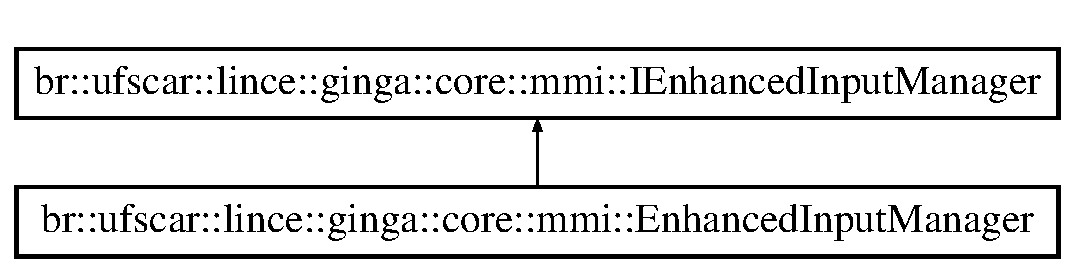
\includegraphics[height=2cm]{classbr_1_1ufscar_1_1lince_1_1ginga_1_1core_1_1mmi_1_1EnhancedInputManager}
\end{center}
\end{figure}
\subsection*{Métodos Públicos}
\begin{DoxyCompactItemize}
\item 
virtual void {\bf release} ()
\item 
virtual void {\bf addInputEventListener} (IInputEventListener $\ast$listener, set$<$ int $>$ $\ast$events=NULL)
\item 
virtual void {\bf removeInputEventListener} (IInputEventListener $\ast$listener)
\item 
virtual void {\bf addApplicationInputEventListener} (IInputEventListener $\ast$listener)
\item 
virtual void {\bf removeApplicationInputEventListener} (IInputEventListener $\ast$listener)
\item 
virtual void {\bf postEvent} (IInputEvent $\ast$event)
\item 
virtual void {\bf postEvent} (int keyCode)
\item 
virtual void {\bf setAxisValues} (int x, int y, int z)
\item 
virtual void {\bf setAxisBoundaries} (int x, int y, int z)
\item 
virtual int {\bf getCurrentXAxisValue} ()
\item 
virtual int {\bf getCurrentYAxisValue} ()
\item 
virtual void {\bf addInputMode} (string inputModeId, {\bf IInputMode} $\ast$inputMode)
\item 
virtual {\bf IInputMode} $\ast$ {\bf removeInputMode} (string inputModeId)
\item 
virtual {\bf IInputMode} $\ast$ {\bf getInputMode} (string inputModeId)
\item 
virtual void {\bf gotoInputMode} (string inputModeId)
\item 
virtual void {\bf addMultimodalInputEventListener} ({\bf IMultimodalInputEventListener} $\ast$listener)
\item 
virtual void {\bf removeMultimodalInputEventListener} ({\bf IMultimodalInputEventListener} $\ast$listener)
\item 
virtual void {\bf postMultimodalEvent} ({\bf IMultimodalInputEvent} $\ast$multimodalInputEvent)
\item 
virtual void {\bf postMultimodalEvent} (string xml)
\item 
virtual int {\bf addCode} (string codeStr)
\item 
virtual bool {\bf removeCode} (int code)
\item 
virtual bool {\bf removeCode} (string codeStr)
\item 
virtual bool {\bf hasCode} (int code)
\item 
virtual bool {\bf hasCode} (string codeStr)
\item 
virtual void {\bf waitForUnlockCondition} ()
\end{DoxyCompactItemize}
\subsection*{Métodos Públicos Estáticos}
\begin{DoxyCompactItemize}
\item 
static {\bf EnhancedInputManager} $\ast$ {\bf getInstance} ()
\end{DoxyCompactItemize}
\subsection*{Métodos Protegidos}
\begin{DoxyCompactItemize}
\item 
{\bf EnhancedInputManager} ()
\item 
{\bf $\sim$EnhancedInputManager} ()
\item 
void {\bf initializeInputIntervalTime} ()
\item 
void {\bf nextInputMode} ()
\item 
virtual bool {\bf dispatchMultimodalEvent} ({\bf IMultimodalInputEvent} $\ast$multimodalInputEvent)
\item 
virtual void {\bf performMultimodalInputLockedActions} ()
\end{DoxyCompactItemize}
\subsection*{Atributos Protegidos}
\begin{DoxyCompactItemize}
\item 
vector$<$ {\bf IInputMode} $\ast$ $>$ $\ast$ {\bf inputModes}\label{classbr_1_1ufscar_1_1lince_1_1ginga_1_1core_1_1mmi_1_1EnhancedInputManager_a6e5fff9b63e9a45109a49f7b95f9205c}

\begin{DoxyCompactList}\small\item\em Conjunto de modos de entrada. \item\end{DoxyCompactList}\item 
map$<$ string, {\bf IInputMode} $\ast$ $>$ $\ast$ {\bf inputModeMap}\label{classbr_1_1ufscar_1_1lince_1_1ginga_1_1core_1_1mmi_1_1EnhancedInputManager_ae7c37f3aae2e48cd1820cc42dc7ca3dc}

\begin{DoxyCompactList}\small\item\em Mapeamento entro o nome do modo de entrada e sua instância. \item\end{DoxyCompactList}\item 
{\bf IInputMode} $\ast$ {\bf currentInputMode}\label{classbr_1_1ufscar_1_1lince_1_1ginga_1_1core_1_1mmi_1_1EnhancedInputManager_aab9106c9072222655fb2865c2121d801}

\begin{DoxyCompactList}\small\item\em Indica o modo de entrada atualmente usado. \item\end{DoxyCompactList}\item 
int {\bf inputModeIndex}\label{classbr_1_1ufscar_1_1lince_1_1ginga_1_1core_1_1mmi_1_1EnhancedInputManager_a17320fd9d0525442ca45f43ead03e1de}

\begin{DoxyCompactList}\small\item\em Indica o índice do modo de entrada atualmente usado. \item\end{DoxyCompactList}\item 
HLoggerPtr {\bf logger}\label{classbr_1_1ufscar_1_1lince_1_1ginga_1_1core_1_1mmi_1_1EnhancedInputManager_ae9f367cfff019213aa973c5e70369bd6}

\begin{DoxyCompactList}\small\item\em Responsável pelo controle das mensagens de log. \item\end{DoxyCompactList}\item 
set$<$ {\bf IMultimodalInputEventListener} $\ast$ $>$ $\ast$ {\bf multimodalEventListeners}\label{classbr_1_1ufscar_1_1lince_1_1ginga_1_1core_1_1mmi_1_1EnhancedInputManager_a20b5337fd0ec2f696a2048bdf633fd94}

\begin{DoxyCompactList}\small\item\em Conjunto de observadores de eventos multimodais. \item\end{DoxyCompactList}\item 
vector$<$ {\bf LockedMultimodalAction} $\ast$ $>$ $\ast$ {\bf actionsToMultimodalListeners}
\item 
bool {\bf notifyingMultimodal}
\item 
pthread\_\-mutex\_\-t {\bf multimodalMutex}\label{classbr_1_1ufscar_1_1lince_1_1ginga_1_1core_1_1mmi_1_1EnhancedInputManager_a803cbbaac8ced4586e74dc72255cb29a}

\begin{DoxyCompactList}\small\item\em Controla o acesso concorrente ao multimodalEventListeners. \item\end{DoxyCompactList}\item 
pthread\_\-mutex\_\-t {\bf actMultimodalMutex}\label{classbr_1_1ufscar_1_1lince_1_1ginga_1_1core_1_1mmi_1_1EnhancedInputManager_a74c2903df33d8ee7d36225b00ab9d906}

\begin{DoxyCompactList}\small\item\em Controla o acesso concorrente ao actionsToMultimodalListeners. \item\end{DoxyCompactList}\item 
CodeMap $\ast$ {\bf codeMap}\label{classbr_1_1ufscar_1_1lince_1_1ginga_1_1core_1_1mmi_1_1EnhancedInputManager_a6809eff2881564b14c89ae01e1372317}

\begin{DoxyCompactList}\small\item\em Instância utilizada para adicionar novos códigos de teclas. \item\end{DoxyCompactList}\item 
map$<$ IInputEventListener $\ast$, set$<$ int $>$ $\ast$ $>$ $\ast$ {\bf eventListeners}
\item 
vector$<$ {\bf LockedAction} $\ast$ $>$ $\ast$ {\bf actionsToInpListeners}
\item 
set$<$ IInputEventListener $\ast$ $>$ $\ast$ {\bf applicationListeners}\label{classbr_1_1ufscar_1_1lince_1_1ginga_1_1core_1_1mmi_1_1EnhancedInputManager_ab1445054a3c2b41ddaca538b05d9e7d4}

\begin{DoxyCompactList}\small\item\em Conjunto de observadores de aplicações. \item\end{DoxyCompactList}\item 
vector$<$ {\bf LockedAction} $\ast$ $>$ $\ast$ {\bf actionsToAppListeners}
\item 
bool {\bf running}\label{classbr_1_1ufscar_1_1lince_1_1ginga_1_1core_1_1mmi_1_1EnhancedInputManager_a43581d244a0e6c4775d10e27d3d34d9b}

\begin{DoxyCompactList}\small\item\em Denota que o InputManager está em execução. \item\end{DoxyCompactList}\item 
bool {\bf notifying}\label{classbr_1_1ufscar_1_1lince_1_1ginga_1_1core_1_1mmi_1_1EnhancedInputManager_a7d1c0dade0b030518232074c800f78a0}

\begin{DoxyCompactList}\small\item\em Denota se o InputManager deve notificar seus listeners. \item\end{DoxyCompactList}\item 
bool {\bf notifyingApp}\label{classbr_1_1ufscar_1_1lince_1_1ginga_1_1core_1_1mmi_1_1EnhancedInputManager_a21a28fdfac85367750774821cd587741}

\begin{DoxyCompactList}\small\item\em Denota se o InputManager deve notificar as aplicações. \item\end{DoxyCompactList}\item 
IEventBuffer $\ast$ {\bf eventBuffer}\label{classbr_1_1ufscar_1_1lince_1_1ginga_1_1core_1_1mmi_1_1EnhancedInputManager_a5d50a61babd99c13e4e714257bffc806}

\begin{DoxyCompactList}\small\item\em Buffer que armazena os eventos que devem ser processados e despachados. \item\end{DoxyCompactList}\item 
double {\bf lastEventTime}\label{classbr_1_1ufscar_1_1lince_1_1ginga_1_1core_1_1mmi_1_1EnhancedInputManager_a9852aa6d23e4856d81df46f36c2d18fa}

\begin{DoxyCompactList}\small\item\em Registra o tempo de ocorrencia do último evento. \item\end{DoxyCompactList}\item 
double {\bf timeStamp}\label{classbr_1_1ufscar_1_1lince_1_1ginga_1_1core_1_1mmi_1_1EnhancedInputManager_a9ccaaefa7388090883593b64c5663c66}

\begin{DoxyCompactList}\small\item\em Utilizado para armazenar o tempo do evento atual. \item\end{DoxyCompactList}\item 
double {\bf imperativeIntervalTime}\label{classbr_1_1ufscar_1_1lince_1_1ginga_1_1core_1_1mmi_1_1EnhancedInputManager_a884bef9c38cb5f8512ac23c4c7dda80e}

\begin{DoxyCompactList}\small\item\em Armazena o intervalo minimo para detectar eventos imperativos. \item\end{DoxyCompactList}\item 
double {\bf declarativeIntervalTime}\label{classbr_1_1ufscar_1_1lince_1_1ginga_1_1core_1_1mmi_1_1EnhancedInputManager_a3f155cda29980c2ee5ba32faa568f814}

\begin{DoxyCompactList}\small\item\em Armazena o intervalo minimo para detectar eventos declarativos. \item\end{DoxyCompactList}\item 
int {\bf currentXAxis}\label{classbr_1_1ufscar_1_1lince_1_1ginga_1_1core_1_1mmi_1_1EnhancedInputManager_a5313a5b41578e9ea0590c01ae4448c23}

\begin{DoxyCompactList}\small\item\em Posição do eixo X atual. \item\end{DoxyCompactList}\item 
int {\bf currentYAxis}\label{classbr_1_1ufscar_1_1lince_1_1ginga_1_1core_1_1mmi_1_1EnhancedInputManager_a778bc03e9d579a4f79b6e9754123422c}

\begin{DoxyCompactList}\small\item\em Posição do eixo Y atual. \item\end{DoxyCompactList}\item 
int {\bf maxX}\label{classbr_1_1ufscar_1_1lince_1_1ginga_1_1core_1_1mmi_1_1EnhancedInputManager_a371866ab633322ef75240da4fe892e2f}

\begin{DoxyCompactList}\small\item\em Valor máximo do eixo X. \item\end{DoxyCompactList}\item 
int {\bf maxY}\label{classbr_1_1ufscar_1_1lince_1_1ginga_1_1core_1_1mmi_1_1EnhancedInputManager_a8100fb2d243ffeaeb72928881f7d5284}

\begin{DoxyCompactList}\small\item\em Valor máximo do eixo Y. \item\end{DoxyCompactList}\item 
pthread\_\-mutex\_\-t {\bf actAppMutex}\label{classbr_1_1ufscar_1_1lince_1_1ginga_1_1core_1_1mmi_1_1EnhancedInputManager_a29d51653cb0fdc17bae852976d162235}

\begin{DoxyCompactList}\small\item\em Controla acesso concorrente à lista actionsToAppListeners. \item\end{DoxyCompactList}\item 
pthread\_\-mutex\_\-t {\bf actInpMutex}\label{classbr_1_1ufscar_1_1lince_1_1ginga_1_1core_1_1mmi_1_1EnhancedInputManager_ae6d773c92a437e94f025d16561bbd74b}

\begin{DoxyCompactList}\small\item\em Controla acesso concorrente à lista actionsToInpListeners. \item\end{DoxyCompactList}\item 
pthread\_\-mutex\_\-t {\bf appMutex}\label{classbr_1_1ufscar_1_1lince_1_1ginga_1_1core_1_1mmi_1_1EnhancedInputManager_a648a33c1a2b3d1ec2d127528db3352a9}

\begin{DoxyCompactList}\small\item\em Controla acesso concorrente à lista applicationListeners. \item\end{DoxyCompactList}\end{DoxyCompactItemize}
\subsection*{Atributos Estáticos Protegidos}
\begin{DoxyCompactItemize}
\item 
static {\bf EnhancedInputManager} $\ast$ {\bf \_\-instance} = NULL\label{classbr_1_1ufscar_1_1lince_1_1ginga_1_1core_1_1mmi_1_1EnhancedInputManager_a0ce47bd3c8357ff0cc0759b602a57196}

\begin{DoxyCompactList}\small\item\em Instância única do \doxyref{EnhancedInputManager}{pag.}{classbr_1_1ufscar_1_1lince_1_1ginga_1_1core_1_1mmi_1_1EnhancedInputManager}. \item\end{DoxyCompactList}\item 
static int {\bf KEY\_\-MODE\_\-CHANGE} = 61968\label{classbr_1_1ufscar_1_1lince_1_1ginga_1_1core_1_1mmi_1_1EnhancedInputManager_a6889b8a679ac4ebef8a0f6ca4cef91d6}

\begin{DoxyCompactList}\small\item\em Código de tecla de um evento que indica mudança do modo de entrada. \item\end{DoxyCompactList}\end{DoxyCompactItemize}


\subsection{Descrição Detalhada}
Essa classe visa substituir o InputManager do componente Ginga-\/CC System IO. Ela implementa a interface IEnhacedInputManager, que estende IInputManager. Essa classe não estende a classe EnhacendInputManager pois assim evitamos: \par

\begin{DoxyItemize}
\item O problema do singleton estendido\par

\item O problema de ter que implementar no EIM métodos que simplesmente servem para chamar os métodos já implementados do IM, pelo fato deles não estarem acessíveis mesmo sendo herdados.\par

\item O problema de o InputManager.h não ser instalado junto com os demais includes do Ginga no sistema. Apenas sua interface IInputManager.h é instalada.\par
 Essa decisão é válida também porque, além de simplificar muito o entendimento do código, quem usa a extensão, não tem mais o menor interesse em ter a versão não estendida em paralelo. 
\end{DoxyItemize}

\subsection{Construtores \& Destrutores}
\index{br::ufscar::lince::ginga::core::mmi::EnhancedInputManager@{br::ufscar::lince::ginga::core::mmi::EnhancedInputManager}!EnhancedInputManager@{EnhancedInputManager}}
\index{EnhancedInputManager@{EnhancedInputManager}!br::ufscar::lince::ginga::core::mmi::EnhancedInputManager@{br::ufscar::lince::ginga::core::mmi::EnhancedInputManager}}
\subsubsection[{EnhancedInputManager}]{\setlength{\rightskip}{0pt plus 5cm}br::ufscar::lince::ginga::core::mmi::EnhancedInputManager::EnhancedInputManager ()\hspace{0.3cm}{\ttfamily  [protected]}}\label{classbr_1_1ufscar_1_1lince_1_1ginga_1_1core_1_1mmi_1_1EnhancedInputManager_ab1332f39609e66bd54fb7649fc8a26b8}
Constrói a instância única do \doxyref{EnhancedInputManager}{pag.}{classbr_1_1ufscar_1_1lince_1_1ginga_1_1core_1_1mmi_1_1EnhancedInputManager} 

Referências actAppMutex, actInpMutex, actionsToAppListeners, actionsToInpListeners, actionsToMultimodalListeners, actMultimodalMutex, applicationListeners, appMutex, codeMap, currentInputMode, currentXAxis, currentYAxis, eventBuffer, eventListeners, getInstance(), initializeInputIntervalTime(), inputModeIndex, inputModeMap, inputModes, lastEventTime, logger, maxX, maxY, multimodalEventListeners, multimodalMutex, notifying, notifyingApp, notifyingMultimodal e running.



Referenciado por getInstance().

\index{br::ufscar::lince::ginga::core::mmi::EnhancedInputManager@{br::ufscar::lince::ginga::core::mmi::EnhancedInputManager}!$\sim$EnhancedInputManager@{$\sim$EnhancedInputManager}}
\index{$\sim$EnhancedInputManager@{$\sim$EnhancedInputManager}!br::ufscar::lince::ginga::core::mmi::EnhancedInputManager@{br::ufscar::lince::ginga::core::mmi::EnhancedInputManager}}
\subsubsection[{$\sim$EnhancedInputManager}]{\setlength{\rightskip}{0pt plus 5cm}br::ufscar::lince::ginga::core::mmi::EnhancedInputManager::$\sim$EnhancedInputManager ()\hspace{0.3cm}{\ttfamily  [protected]}}\label{classbr_1_1ufscar_1_1lince_1_1ginga_1_1core_1_1mmi_1_1EnhancedInputManager_aff3634c4d9a2cb034394fdd24bf31c8e}
Destrói o \doxyref{EnhancedInputManager}{pag.}{classbr_1_1ufscar_1_1lince_1_1ginga_1_1core_1_1mmi_1_1EnhancedInputManager}. 

Referências \_\-instance e logger.



\subsection{Métodos}
\index{br::ufscar::lince::ginga::core::mmi::EnhancedInputManager@{br::ufscar::lince::ginga::core::mmi::EnhancedInputManager}!addApplicationInputEventListener@{addApplicationInputEventListener}}
\index{addApplicationInputEventListener@{addApplicationInputEventListener}!br::ufscar::lince::ginga::core::mmi::EnhancedInputManager@{br::ufscar::lince::ginga::core::mmi::EnhancedInputManager}}
\subsubsection[{addApplicationInputEventListener}]{\setlength{\rightskip}{0pt plus 5cm}void br::ufscar::lince::ginga::core::mmi::EnhancedInputManager::addApplicationInputEventListener (IInputEventListener $\ast$ {\em listener})\hspace{0.3cm}{\ttfamily  [virtual]}}\label{classbr_1_1ufscar_1_1lince_1_1ginga_1_1core_1_1mmi_1_1EnhancedInputManager_a134d1ab1b40af56590bd10d0fe5f4e74}
Registra um observador de eventos de aplicação. 
\begin{DoxyParams}{Parâmetros}
\item[{\em listener}]O observador a ser registrado. \end{DoxyParams}


Referências actAppMutex, actionsToAppListeners, applicationListeners, appMutex, lockedListenerAction::events, lockedListenerAction::isAdd, lockedListenerAction::l, notifyingApp e running.

\index{br::ufscar::lince::ginga::core::mmi::EnhancedInputManager@{br::ufscar::lince::ginga::core::mmi::EnhancedInputManager}!addCode@{addCode}}
\index{addCode@{addCode}!br::ufscar::lince::ginga::core::mmi::EnhancedInputManager@{br::ufscar::lince::ginga::core::mmi::EnhancedInputManager}}
\subsubsection[{addCode}]{\setlength{\rightskip}{0pt plus 5cm}int br::ufscar::lince::ginga::core::mmi::EnhancedInputManager::addCode (string {\em codeStr})\hspace{0.3cm}{\ttfamily  [virtual]}}\label{classbr_1_1ufscar_1_1lince_1_1ginga_1_1core_1_1mmi_1_1EnhancedInputManager_ae712d436ac1e9a101ac83051905db21b}
Adiciona um novo código de tecla. 
\begin{DoxyParams}{Parâmetros}
\item[{\em codeStr}]Identificador da nova tecla. \end{DoxyParams}
\begin{DoxyReturn}{Retorna}
Código atribuido à tecla. 
\end{DoxyReturn}


Implementa {\bf br::ufscar::lince::ginga::core::mmi::IEnhancedInputManager} \doxyref{}{pag.}{classbr_1_1ufscar_1_1lince_1_1ginga_1_1core_1_1mmi_1_1IEnhancedInputManager_abd69b86a5205125e16ff3498f9fbcc6e}.



Referências codeMap.

\index{br::ufscar::lince::ginga::core::mmi::EnhancedInputManager@{br::ufscar::lince::ginga::core::mmi::EnhancedInputManager}!addInputEventListener@{addInputEventListener}}
\index{addInputEventListener@{addInputEventListener}!br::ufscar::lince::ginga::core::mmi::EnhancedInputManager@{br::ufscar::lince::ginga::core::mmi::EnhancedInputManager}}
\subsubsection[{addInputEventListener}]{\setlength{\rightskip}{0pt plus 5cm}void br::ufscar::lince::ginga::core::mmi::EnhancedInputManager::addInputEventListener (IInputEventListener $\ast$ {\em listener}, \/  set$<$ int $>$ $\ast$ {\em events} = {\ttfamily NULL})\hspace{0.3cm}{\ttfamily  [virtual]}}\label{classbr_1_1ufscar_1_1lince_1_1ginga_1_1core_1_1mmi_1_1EnhancedInputManager_ab962318f78d6303ad28cabf5ae17f53c}
Registra um observador de eventos. 
\begin{DoxyParams}{Parâmetros}
\item[{\em listener}]O observador a ser registrado. \item[{\em events}]Conjunto de eventos de interesse. \end{DoxyParams}


Referências actInpMutex, actionsToInpListeners, eventListeners, lockedListenerAction::events, lockedListenerAction::isAdd, lockedListenerAction::l, notifying e running.

\index{br::ufscar::lince::ginga::core::mmi::EnhancedInputManager@{br::ufscar::lince::ginga::core::mmi::EnhancedInputManager}!addInputMode@{addInputMode}}
\index{addInputMode@{addInputMode}!br::ufscar::lince::ginga::core::mmi::EnhancedInputManager@{br::ufscar::lince::ginga::core::mmi::EnhancedInputManager}}
\subsubsection[{addInputMode}]{\setlength{\rightskip}{0pt plus 5cm}void br::ufscar::lince::ginga::core::mmi::EnhancedInputManager::addInputMode (string {\em inputModeId}, \/  {\bf IInputMode} $\ast$ {\em inputMode})\hspace{0.3cm}{\ttfamily  [virtual]}}\label{classbr_1_1ufscar_1_1lince_1_1ginga_1_1core_1_1mmi_1_1EnhancedInputManager_a9f2d1868f1a67f2f51e1df07484d5be1}
Adicina um novo modo de entrada. 
\begin{DoxyParams}{Parâmetros}
\item[{\em inputModeId}]Id do novo modo de entrada. \item[{\em inputMode}]Novo modo de entrada. \end{DoxyParams}

\begin{DoxyExceptions}{Exceções}
\item[{\em BadArgumentException}]se inputMode for nulo. \item[{\em \doxyref{DuplicateException}{pag.}{classbr_1_1ufscar_1_1lince_1_1ginga_1_1core_1_1mmi_1_1DuplicateException}}]se outro modo já adicionado possuir inputModeName como identificador. \end{DoxyExceptions}


Implementa {\bf br::ufscar::lince::ginga::core::mmi::IEnhancedInputManager} \doxyref{}{pag.}{classbr_1_1ufscar_1_1lince_1_1ginga_1_1core_1_1mmi_1_1IEnhancedInputManager_ac3620e81bb403ee7468de5752095ac0a}.



Referências inputModeMap, inputModes e logger.

\index{br::ufscar::lince::ginga::core::mmi::EnhancedInputManager@{br::ufscar::lince::ginga::core::mmi::EnhancedInputManager}!addMultimodalInputEventListener@{addMultimodalInputEventListener}}
\index{addMultimodalInputEventListener@{addMultimodalInputEventListener}!br::ufscar::lince::ginga::core::mmi::EnhancedInputManager@{br::ufscar::lince::ginga::core::mmi::EnhancedInputManager}}
\subsubsection[{addMultimodalInputEventListener}]{\setlength{\rightskip}{0pt plus 5cm}void br::ufscar::lince::ginga::core::mmi::EnhancedInputManager::addMultimodalInputEventListener ({\bf IMultimodalInputEventListener} $\ast$ {\em listener})\hspace{0.3cm}{\ttfamily  [virtual]}}\label{classbr_1_1ufscar_1_1lince_1_1ginga_1_1core_1_1mmi_1_1EnhancedInputManager_af2f533b4ca43c0df2f712ef04183d166}
Registra um observador de eventos multimodais. 
\begin{DoxyParams}{Parâmetros}
\item[{\em listener}]O observador a ser registrado. \end{DoxyParams}


Implementa {\bf br::ufscar::lince::ginga::core::mmi::IEnhancedInputManager} \doxyref{}{pag.}{classbr_1_1ufscar_1_1lince_1_1ginga_1_1core_1_1mmi_1_1IEnhancedInputManager_a5be22768c393249571ded39e79ed8dda}.



Referências actionsToMultimodalListeners, actMultimodalMutex, lockedMultimodalListenerAction::isAdd, lockedMultimodalListenerAction::l, logger, multimodalEventListeners, multimodalMutex, notifying, performMultimodalInputLockedActions() e running.

\index{br::ufscar::lince::ginga::core::mmi::EnhancedInputManager@{br::ufscar::lince::ginga::core::mmi::EnhancedInputManager}!dispatchMultimodalEvent@{dispatchMultimodalEvent}}
\index{dispatchMultimodalEvent@{dispatchMultimodalEvent}!br::ufscar::lince::ginga::core::mmi::EnhancedInputManager@{br::ufscar::lince::ginga::core::mmi::EnhancedInputManager}}
\subsubsection[{dispatchMultimodalEvent}]{\setlength{\rightskip}{0pt plus 5cm}bool br::ufscar::lince::ginga::core::mmi::EnhancedInputManager::dispatchMultimodalEvent ({\bf IMultimodalInputEvent} $\ast$ {\em multimodalInputEvent})\hspace{0.3cm}{\ttfamily  [protected, virtual]}}\label{classbr_1_1ufscar_1_1lince_1_1ginga_1_1core_1_1mmi_1_1EnhancedInputManager_a67b3b8dcf42c63ad7ee9914521eaacc7}
Notifica os observadores da ocorrência de um evento multimodal. 
\begin{DoxyParams}{Parâmetros}
\item[{\em multimodalInputEvent}]Evento sendo notificado. \end{DoxyParams}


Referências logger, multimodalEventListeners, multimodalMutex, notifying, notifyingMultimodal, performMultimodalInputLockedActions() e running.

\index{br::ufscar::lince::ginga::core::mmi::EnhancedInputManager@{br::ufscar::lince::ginga::core::mmi::EnhancedInputManager}!getCurrentXAxisValue@{getCurrentXAxisValue}}
\index{getCurrentXAxisValue@{getCurrentXAxisValue}!br::ufscar::lince::ginga::core::mmi::EnhancedInputManager@{br::ufscar::lince::ginga::core::mmi::EnhancedInputManager}}
\subsubsection[{getCurrentXAxisValue}]{\setlength{\rightskip}{0pt plus 5cm}int br::ufscar::lince::ginga::core::mmi::EnhancedInputManager::getCurrentXAxisValue ()\hspace{0.3cm}{\ttfamily  [virtual]}}\label{classbr_1_1ufscar_1_1lince_1_1ginga_1_1core_1_1mmi_1_1EnhancedInputManager_a323118f859ef613f681321e7a80277d4}
Acessa a posição atual do ponteiro do mouse na coordenada x. \begin{DoxyReturn}{Retorna}
A posição atual do ponteiro do mouse na coordenada x. 
\end{DoxyReturn}


Referências currentXAxis.

\index{br::ufscar::lince::ginga::core::mmi::EnhancedInputManager@{br::ufscar::lince::ginga::core::mmi::EnhancedInputManager}!getCurrentYAxisValue@{getCurrentYAxisValue}}
\index{getCurrentYAxisValue@{getCurrentYAxisValue}!br::ufscar::lince::ginga::core::mmi::EnhancedInputManager@{br::ufscar::lince::ginga::core::mmi::EnhancedInputManager}}
\subsubsection[{getCurrentYAxisValue}]{\setlength{\rightskip}{0pt plus 5cm}int br::ufscar::lince::ginga::core::mmi::EnhancedInputManager::getCurrentYAxisValue ()\hspace{0.3cm}{\ttfamily  [virtual]}}\label{classbr_1_1ufscar_1_1lince_1_1ginga_1_1core_1_1mmi_1_1EnhancedInputManager_aed7edfbbd1c856b97bfa01fedab77709}
Acessa a posição atual do ponteiro do mouse na coordenada y. \begin{DoxyReturn}{Retorna}
A posição atual do ponteiro do mouse na coordenada y. 
\end{DoxyReturn}


Referências currentYAxis.

\index{br::ufscar::lince::ginga::core::mmi::EnhancedInputManager@{br::ufscar::lince::ginga::core::mmi::EnhancedInputManager}!getInputMode@{getInputMode}}
\index{getInputMode@{getInputMode}!br::ufscar::lince::ginga::core::mmi::EnhancedInputManager@{br::ufscar::lince::ginga::core::mmi::EnhancedInputManager}}
\subsubsection[{getInputMode}]{\setlength{\rightskip}{0pt plus 5cm}{\bf IInputMode} $\ast$ br::ufscar::lince::ginga::core::mmi::EnhancedInputManager::getInputMode (string {\em inputModeId})\hspace{0.3cm}{\ttfamily  [virtual]}}\label{classbr_1_1ufscar_1_1lince_1_1ginga_1_1core_1_1mmi_1_1EnhancedInputManager_a6d3cd7e5533be32dc80f1f8659bd5920}
Acessa um modo de entrada previamente adicionado. 
\begin{DoxyParams}{Parâmetros}
\item[{\em inputModeId}]Id do modo de entrada a ser acessado. \end{DoxyParams}
\begin{DoxyReturn}{Retorna}
O modo de entrada ou NULL caso o modo não seja encontrado. 
\end{DoxyReturn}


Implementa {\bf br::ufscar::lince::ginga::core::mmi::IEnhancedInputManager} \doxyref{}{pag.}{classbr_1_1ufscar_1_1lince_1_1ginga_1_1core_1_1mmi_1_1IEnhancedInputManager_acef61e560c6a3576d4530ce6c8db125a}.



Referências inputModeMap e logger.



Referenciado por gotoInputMode().

\index{br::ufscar::lince::ginga::core::mmi::EnhancedInputManager@{br::ufscar::lince::ginga::core::mmi::EnhancedInputManager}!getInstance@{getInstance}}
\index{getInstance@{getInstance}!br::ufscar::lince::ginga::core::mmi::EnhancedInputManager@{br::ufscar::lince::ginga::core::mmi::EnhancedInputManager}}
\subsubsection[{getInstance}]{\setlength{\rightskip}{0pt plus 5cm}{\bf EnhancedInputManager} $\ast$ br::ufscar::lince::ginga::core::mmi::EnhancedInputManager::getInstance ()\hspace{0.3cm}{\ttfamily  [static]}}\label{classbr_1_1ufscar_1_1lince_1_1ginga_1_1core_1_1mmi_1_1EnhancedInputManager_a50781e4a3b4d17d99614f267e098be4e}
Acessa a instância única do \doxyref{EnhancedInputManager}{pag.}{classbr_1_1ufscar_1_1lince_1_1ginga_1_1core_1_1mmi_1_1EnhancedInputManager}. 

Referências \_\-instance e EnhancedInputManager().



Referenciado por EnhancedInputManager() e postMultimodalEvent().

\index{br::ufscar::lince::ginga::core::mmi::EnhancedInputManager@{br::ufscar::lince::ginga::core::mmi::EnhancedInputManager}!gotoInputMode@{gotoInputMode}}
\index{gotoInputMode@{gotoInputMode}!br::ufscar::lince::ginga::core::mmi::EnhancedInputManager@{br::ufscar::lince::ginga::core::mmi::EnhancedInputManager}}
\subsubsection[{gotoInputMode}]{\setlength{\rightskip}{0pt plus 5cm}void br::ufscar::lince::ginga::core::mmi::EnhancedInputManager::gotoInputMode (string {\em inputModeId})\hspace{0.3cm}{\ttfamily  [virtual]}}\label{classbr_1_1ufscar_1_1lince_1_1ginga_1_1core_1_1mmi_1_1EnhancedInputManager_a516c9e18cabe5b1daab04c5fd73d5eaa}
Atvia um modo de entrada previamente adicionado. 
\begin{DoxyParams}{Parâmetros}
\item[{\em inputModeId}]Id do modo de entrada a ser ativado. \end{DoxyParams}


Implementa {\bf br::ufscar::lince::ginga::core::mmi::IEnhancedInputManager} \doxyref{}{pag.}{classbr_1_1ufscar_1_1lince_1_1ginga_1_1core_1_1mmi_1_1IEnhancedInputManager_a09a9c5af4124bc571515e94f68b07256}.



Referências currentInputMode, getInputMode(), inputModeIndex, inputModes e logger.

\index{br::ufscar::lince::ginga::core::mmi::EnhancedInputManager@{br::ufscar::lince::ginga::core::mmi::EnhancedInputManager}!hasCode@{hasCode}}
\index{hasCode@{hasCode}!br::ufscar::lince::ginga::core::mmi::EnhancedInputManager@{br::ufscar::lince::ginga::core::mmi::EnhancedInputManager}}
\subsubsection[{hasCode}]{\setlength{\rightskip}{0pt plus 5cm}bool br::ufscar::lince::ginga::core::mmi::EnhancedInputManager::hasCode (string {\em codeStr})\hspace{0.3cm}{\ttfamily  [virtual]}}\label{classbr_1_1ufscar_1_1lince_1_1ginga_1_1core_1_1mmi_1_1EnhancedInputManager_a2e66b0f723f9abb5f9589f56d1e21d75}
Verifica se uma dada tecla existe no conjunto de teclas mapeadas. 
\begin{DoxyParams}{Parâmetros}
\item[{\em codeStr}]Identificador da tecla a ser chegada. \end{DoxyParams}
\begin{DoxyReturn}{Retorna}
true se a tecla existir; false caso contrário. 
\end{DoxyReturn}


Implementa {\bf br::ufscar::lince::ginga::core::mmi::IEnhancedInputManager} \doxyref{}{pag.}{classbr_1_1ufscar_1_1lince_1_1ginga_1_1core_1_1mmi_1_1IEnhancedInputManager_a1d998e5010e297c48ae13fc47c9c5234}.



Referências codeMap.

\index{br::ufscar::lince::ginga::core::mmi::EnhancedInputManager@{br::ufscar::lince::ginga::core::mmi::EnhancedInputManager}!hasCode@{hasCode}}
\index{hasCode@{hasCode}!br::ufscar::lince::ginga::core::mmi::EnhancedInputManager@{br::ufscar::lince::ginga::core::mmi::EnhancedInputManager}}
\subsubsection[{hasCode}]{\setlength{\rightskip}{0pt plus 5cm}bool br::ufscar::lince::ginga::core::mmi::EnhancedInputManager::hasCode (int {\em code})\hspace{0.3cm}{\ttfamily  [virtual]}}\label{classbr_1_1ufscar_1_1lince_1_1ginga_1_1core_1_1mmi_1_1EnhancedInputManager_a41b5236e73086da4ad199087f00f7b5b}
Verifica se uma dada tecla existe no conjunto de teclas mapeadas. 
\begin{DoxyParams}{Parâmetros}
\item[{\em code}]Código da tecla a ser chegada. \end{DoxyParams}
\begin{DoxyReturn}{Retorna}
true se a tecla existir; false caso contrário. 
\end{DoxyReturn}


Implementa {\bf br::ufscar::lince::ginga::core::mmi::IEnhancedInputManager} \doxyref{}{pag.}{classbr_1_1ufscar_1_1lince_1_1ginga_1_1core_1_1mmi_1_1IEnhancedInputManager_ad60eb6cadce0c06f8b1ac07528635d0c}.



Referências codeMap.

\index{br::ufscar::lince::ginga::core::mmi::EnhancedInputManager@{br::ufscar::lince::ginga::core::mmi::EnhancedInputManager}!initializeInputIntervalTime@{initializeInputIntervalTime}}
\index{initializeInputIntervalTime@{initializeInputIntervalTime}!br::ufscar::lince::ginga::core::mmi::EnhancedInputManager@{br::ufscar::lince::ginga::core::mmi::EnhancedInputManager}}
\subsubsection[{initializeInputIntervalTime}]{\setlength{\rightskip}{0pt plus 5cm}void br::ufscar::lince::ginga::core::mmi::EnhancedInputManager::initializeInputIntervalTime ()\hspace{0.3cm}{\ttfamily  [protected]}}\label{classbr_1_1ufscar_1_1lince_1_1ginga_1_1core_1_1mmi_1_1EnhancedInputManager_a19b7095d9f0684a37d04d39950483fb6}
Lê do arquivo de configuração os intervalos de tempo mínimos para que dois eventos da mesma tecla sejam considerados. 

Referências declarativeIntervalTime, imperativeIntervalTime e logger.



Referenciado por EnhancedInputManager().

\index{br::ufscar::lince::ginga::core::mmi::EnhancedInputManager@{br::ufscar::lince::ginga::core::mmi::EnhancedInputManager}!nextInputMode@{nextInputMode}}
\index{nextInputMode@{nextInputMode}!br::ufscar::lince::ginga::core::mmi::EnhancedInputManager@{br::ufscar::lince::ginga::core::mmi::EnhancedInputManager}}
\subsubsection[{nextInputMode}]{\setlength{\rightskip}{0pt plus 5cm}void br::ufscar::lince::ginga::core::mmi::EnhancedInputManager::nextInputMode ()\hspace{0.3cm}{\ttfamily  [protected]}}\label{classbr_1_1ufscar_1_1lince_1_1ginga_1_1core_1_1mmi_1_1EnhancedInputManager_ade89a1f7a566a6d8afaa68110476e7e8}
Alterna para o próximo modo de entrada registrado, caso algum outro modo exista. 

Referências currentInputMode, br::ufscar::lince::ginga::core::mmi::IInputMode::exitingInputMode(), inputModeIndex, inputModes, logger e br::ufscar::lince::ginga::core::mmi::IInputMode::startingInputMode().

\index{br::ufscar::lince::ginga::core::mmi::EnhancedInputManager@{br::ufscar::lince::ginga::core::mmi::EnhancedInputManager}!performMultimodalInputLockedActions@{performMultimodalInputLockedActions}}
\index{performMultimodalInputLockedActions@{performMultimodalInputLockedActions}!br::ufscar::lince::ginga::core::mmi::EnhancedInputManager@{br::ufscar::lince::ginga::core::mmi::EnhancedInputManager}}
\subsubsection[{performMultimodalInputLockedActions}]{\setlength{\rightskip}{0pt plus 5cm}void br::ufscar::lince::ginga::core::mmi::EnhancedInputManager::performMultimodalInputLockedActions ()\hspace{0.3cm}{\ttfamily  [protected, virtual]}}\label{classbr_1_1ufscar_1_1lince_1_1ginga_1_1core_1_1mmi_1_1EnhancedInputManager_a333c7ee7dbe92aaa064fc04d06c05946}
Atualiza o conjunto multimodalEventListeners com base na lista de ações de adição e remoção de listeners (actionsToMultimodalListeners). 

Referências actionsToMultimodalListeners, actMultimodalMutex, lockedMultimodalListenerAction::isAdd, lockedMultimodalListenerAction::l, logger, multimodalEventListeners e running.



Referenciado por addMultimodalInputEventListener(), dispatchMultimodalEvent() e removeMultimodalInputEventListener().

\index{br::ufscar::lince::ginga::core::mmi::EnhancedInputManager@{br::ufscar::lince::ginga::core::mmi::EnhancedInputManager}!postEvent@{postEvent}}
\index{postEvent@{postEvent}!br::ufscar::lince::ginga::core::mmi::EnhancedInputManager@{br::ufscar::lince::ginga::core::mmi::EnhancedInputManager}}
\subsubsection[{postEvent}]{\setlength{\rightskip}{0pt plus 5cm}void br::ufscar::lince::ginga::core::mmi::EnhancedInputManager::postEvent (int {\em keyCode})\hspace{0.3cm}{\ttfamily  [virtual]}}\label{classbr_1_1ufscar_1_1lince_1_1ginga_1_1core_1_1mmi_1_1EnhancedInputManager_a4c9d54eb3e386e6fa444b25272182f64}
Permite a notificação a ocorrência de um evento. 
\begin{DoxyParams}{Parâmetros}
\item[{\em keyCode}]Tecla pressionada. \end{DoxyParams}


Referências postEvent().

\index{br::ufscar::lince::ginga::core::mmi::EnhancedInputManager@{br::ufscar::lince::ginga::core::mmi::EnhancedInputManager}!postEvent@{postEvent}}
\index{postEvent@{postEvent}!br::ufscar::lince::ginga::core::mmi::EnhancedInputManager@{br::ufscar::lince::ginga::core::mmi::EnhancedInputManager}}
\subsubsection[{postEvent}]{\setlength{\rightskip}{0pt plus 5cm}void br::ufscar::lince::ginga::core::mmi::EnhancedInputManager::postEvent (IInputEvent $\ast$ {\em event})\hspace{0.3cm}{\ttfamily  [virtual]}}\label{classbr_1_1ufscar_1_1lince_1_1ginga_1_1core_1_1mmi_1_1EnhancedInputManager_ae9d739785faff39a808130d1c84a0293}
Permite a notificação da ocorrência de um evento. 
\begin{DoxyParams}{Parâmetros}
\item[{\em event}]O evento ocorrido. \end{DoxyParams}


Referências eventBuffer, logger e running.



Referenciado por postEvent() e postMultimodalEvent().

\index{br::ufscar::lince::ginga::core::mmi::EnhancedInputManager@{br::ufscar::lince::ginga::core::mmi::EnhancedInputManager}!postMultimodalEvent@{postMultimodalEvent}}
\index{postMultimodalEvent@{postMultimodalEvent}!br::ufscar::lince::ginga::core::mmi::EnhancedInputManager@{br::ufscar::lince::ginga::core::mmi::EnhancedInputManager}}
\subsubsection[{postMultimodalEvent}]{\setlength{\rightskip}{0pt plus 5cm}void br::ufscar::lince::ginga::core::mmi::EnhancedInputManager::postMultimodalEvent (string {\em xml})\hspace{0.3cm}{\ttfamily  [virtual]}}\label{classbr_1_1ufscar_1_1lince_1_1ginga_1_1core_1_1mmi_1_1EnhancedInputManager_ac54fd185c441d02b9a925c366c4de866}
Permite a notificação da ocorrência de um evento multimodal na forma de uma string contendo um xml. Essa função faz o parser do xml, monta um objeto de evento multimodal e chama o método void \doxyref{postMultimodalEvent(IMultimodalInputEvent$\ast$ multimodalInputEvent)}{pag.}{classbr_1_1ufscar_1_1lince_1_1ginga_1_1core_1_1mmi_1_1EnhancedInputManager_a6e2e28a5aa71bef5d112ad03219caa40} 
\begin{DoxyParams}{Parâmetros}
\item[{\em xml}]O evento multimodal ocorrido em formato xml. \end{DoxyParams}


Implementa {\bf br::ufscar::lince::ginga::core::mmi::IEnhancedInputManager} \doxyref{}{pag.}{classbr_1_1ufscar_1_1lince_1_1ginga_1_1core_1_1mmi_1_1IEnhancedInputManager_a164d3b69f779481390962b44e2e30c3c}.



Referências br::ufscar::lince::ginga::core::mmi::IMultimodalInputEvent::getId(), getInstance(), logger, br::ufscar::lince::ginga::core::mmi::EventParser::parse(), postEvent() e postMultimodalEvent().

\index{br::ufscar::lince::ginga::core::mmi::EnhancedInputManager@{br::ufscar::lince::ginga::core::mmi::EnhancedInputManager}!postMultimodalEvent@{postMultimodalEvent}}
\index{postMultimodalEvent@{postMultimodalEvent}!br::ufscar::lince::ginga::core::mmi::EnhancedInputManager@{br::ufscar::lince::ginga::core::mmi::EnhancedInputManager}}
\subsubsection[{postMultimodalEvent}]{\setlength{\rightskip}{0pt plus 5cm}void br::ufscar::lince::ginga::core::mmi::EnhancedInputManager::postMultimodalEvent ({\bf IMultimodalInputEvent} $\ast$ {\em multimodalInputEvent})\hspace{0.3cm}{\ttfamily  [virtual]}}\label{classbr_1_1ufscar_1_1lince_1_1ginga_1_1core_1_1mmi_1_1EnhancedInputManager_a6e2e28a5aa71bef5d112ad03219caa40}
Permite a notificação a ocorrência de um evento multimodal. 
\begin{DoxyParams}{Parâmetros}
\item[{\em multimodalInputEvent}]O evento multimodal ocorrido. \end{DoxyParams}


Implementa {\bf br::ufscar::lince::ginga::core::mmi::IEnhancedInputManager} \doxyref{}{pag.}{classbr_1_1ufscar_1_1lince_1_1ginga_1_1core_1_1mmi_1_1IEnhancedInputManager_a1b294030cfc45c78836c05488f95582a}.



Referências logger e postEvent().



Referenciado por postMultimodalEvent().

\index{br::ufscar::lince::ginga::core::mmi::EnhancedInputManager@{br::ufscar::lince::ginga::core::mmi::EnhancedInputManager}!release@{release}}
\index{release@{release}!br::ufscar::lince::ginga::core::mmi::EnhancedInputManager@{br::ufscar::lince::ginga::core::mmi::EnhancedInputManager}}
\subsubsection[{release}]{\setlength{\rightskip}{0pt plus 5cm}void br::ufscar::lince::ginga::core::mmi::EnhancedInputManager::release ()\hspace{0.3cm}{\ttfamily  [virtual]}}\label{classbr_1_1ufscar_1_1lince_1_1ginga_1_1core_1_1mmi_1_1EnhancedInputManager_aede072c9019d453a866ff8fca58b46f0}
Esvazia as listas de listeners e deleta o buffer de eventos. 

Referências actAppMutex, actInpMutex, actionsToAppListeners, actionsToInpListeners, actionsToMultimodalListeners, actMultimodalMutex, applicationListeners, appMutex, eventBuffer, eventListeners, logger, multimodalEventListeners, multimodalMutex, notifying, notifyingApp, notifyingMultimodal e running.

\index{br::ufscar::lince::ginga::core::mmi::EnhancedInputManager@{br::ufscar::lince::ginga::core::mmi::EnhancedInputManager}!removeApplicationInputEventListener@{removeApplicationInputEventListener}}
\index{removeApplicationInputEventListener@{removeApplicationInputEventListener}!br::ufscar::lince::ginga::core::mmi::EnhancedInputManager@{br::ufscar::lince::ginga::core::mmi::EnhancedInputManager}}
\subsubsection[{removeApplicationInputEventListener}]{\setlength{\rightskip}{0pt plus 5cm}void br::ufscar::lince::ginga::core::mmi::EnhancedInputManager::removeApplicationInputEventListener (IInputEventListener $\ast$ {\em listener})\hspace{0.3cm}{\ttfamily  [virtual]}}\label{classbr_1_1ufscar_1_1lince_1_1ginga_1_1core_1_1mmi_1_1EnhancedInputManager_af27454e8d673137d51e9729fc02f65e2}
Remove um observador de eventos de aplicação. 
\begin{DoxyParams}{Parâmetros}
\item[{\em listener}]O observador a ser removido. \end{DoxyParams}


Referências actAppMutex, actionsToAppListeners, applicationListeners, appMutex, lockedListenerAction::events, lockedListenerAction::isAdd, lockedListenerAction::l, notifyingApp e running.

\index{br::ufscar::lince::ginga::core::mmi::EnhancedInputManager@{br::ufscar::lince::ginga::core::mmi::EnhancedInputManager}!removeCode@{removeCode}}
\index{removeCode@{removeCode}!br::ufscar::lince::ginga::core::mmi::EnhancedInputManager@{br::ufscar::lince::ginga::core::mmi::EnhancedInputManager}}
\subsubsection[{removeCode}]{\setlength{\rightskip}{0pt plus 5cm}bool br::ufscar::lince::ginga::core::mmi::EnhancedInputManager::removeCode (string {\em codeStr})\hspace{0.3cm}{\ttfamily  [virtual]}}\label{classbr_1_1ufscar_1_1lince_1_1ginga_1_1core_1_1mmi_1_1EnhancedInputManager_afe3a5063ea99cb766543c4a2c1054ec2}
Remove uma tecla do conjunto de teclas mapeadas. 
\begin{DoxyParams}{Parâmetros}
\item[{\em codeStr}]Identificador a ser removida. \end{DoxyParams}
\begin{DoxyReturn}{Retorna}
true se a tecla foi removida com sucesso; false caso contrário. 
\end{DoxyReturn}


Implementa {\bf br::ufscar::lince::ginga::core::mmi::IEnhancedInputManager} \doxyref{}{pag.}{classbr_1_1ufscar_1_1lince_1_1ginga_1_1core_1_1mmi_1_1IEnhancedInputManager_a4d29e5e24c0a0fefbae57dee15113c53}.



Referências codeMap.

\index{br::ufscar::lince::ginga::core::mmi::EnhancedInputManager@{br::ufscar::lince::ginga::core::mmi::EnhancedInputManager}!removeCode@{removeCode}}
\index{removeCode@{removeCode}!br::ufscar::lince::ginga::core::mmi::EnhancedInputManager@{br::ufscar::lince::ginga::core::mmi::EnhancedInputManager}}
\subsubsection[{removeCode}]{\setlength{\rightskip}{0pt plus 5cm}bool br::ufscar::lince::ginga::core::mmi::EnhancedInputManager::removeCode (int {\em code})\hspace{0.3cm}{\ttfamily  [virtual]}}\label{classbr_1_1ufscar_1_1lince_1_1ginga_1_1core_1_1mmi_1_1EnhancedInputManager_a1d4a7473ddef29b2bd933293f8ed30b8}
Remove uma tecla do conjunto de teclas mapeadas. 
\begin{DoxyParams}{Parâmetros}
\item[{\em code}]Código da tecla a ser removida. \end{DoxyParams}
\begin{DoxyReturn}{Retorna}
true se a tecla foi removida com sucesso; false caso contrário. 
\end{DoxyReturn}


Implementa {\bf br::ufscar::lince::ginga::core::mmi::IEnhancedInputManager} \doxyref{}{pag.}{classbr_1_1ufscar_1_1lince_1_1ginga_1_1core_1_1mmi_1_1IEnhancedInputManager_a7d16d1b63d954ebf7c29e75dd8ea60ec}.



Referências codeMap.

\index{br::ufscar::lince::ginga::core::mmi::EnhancedInputManager@{br::ufscar::lince::ginga::core::mmi::EnhancedInputManager}!removeInputEventListener@{removeInputEventListener}}
\index{removeInputEventListener@{removeInputEventListener}!br::ufscar::lince::ginga::core::mmi::EnhancedInputManager@{br::ufscar::lince::ginga::core::mmi::EnhancedInputManager}}
\subsubsection[{removeInputEventListener}]{\setlength{\rightskip}{0pt plus 5cm}void br::ufscar::lince::ginga::core::mmi::EnhancedInputManager::removeInputEventListener (IInputEventListener $\ast$ {\em listener})\hspace{0.3cm}{\ttfamily  [virtual]}}\label{classbr_1_1ufscar_1_1lince_1_1ginga_1_1core_1_1mmi_1_1EnhancedInputManager_a2a18be127f2547ea1f29855618071ba6}
Remove um observador de eventos. 
\begin{DoxyParams}{Parâmetros}
\item[{\em listener}]O observador a ser removido. \end{DoxyParams}


Referências actInpMutex, actionsToInpListeners, eventListeners, lockedListenerAction::events, lockedListenerAction::isAdd, lockedListenerAction::l, notifying e running.

\index{br::ufscar::lince::ginga::core::mmi::EnhancedInputManager@{br::ufscar::lince::ginga::core::mmi::EnhancedInputManager}!removeInputMode@{removeInputMode}}
\index{removeInputMode@{removeInputMode}!br::ufscar::lince::ginga::core::mmi::EnhancedInputManager@{br::ufscar::lince::ginga::core::mmi::EnhancedInputManager}}
\subsubsection[{removeInputMode}]{\setlength{\rightskip}{0pt plus 5cm}{\bf IInputMode} $\ast$ br::ufscar::lince::ginga::core::mmi::EnhancedInputManager::removeInputMode (string {\em inputModeId})\hspace{0.3cm}{\ttfamily  [virtual]}}\label{classbr_1_1ufscar_1_1lince_1_1ginga_1_1core_1_1mmi_1_1EnhancedInputManager_ac8344e0a6779dff8ff9113482b39581b}
Remove um modo de entrada previamente adicionado. 
\begin{DoxyParams}{Parâmetros}
\item[{\em inputModeId}]Id do modo de entrada a ser removido. \end{DoxyParams}
\begin{DoxyReturn}{Retorna}
O modo de entrada removido ou NULL caso o modo não seja encontrado. 
\end{DoxyReturn}

\begin{DoxyExceptions}{Exceções}
\item[{\em BadArgumentException}]inputModeName for o identificador do modo de entrada atual. \end{DoxyExceptions}


Implementa {\bf br::ufscar::lince::ginga::core::mmi::IEnhancedInputManager} \doxyref{}{pag.}{classbr_1_1ufscar_1_1lince_1_1ginga_1_1core_1_1mmi_1_1IEnhancedInputManager_ad4b902e0a85aa2d0fe3df51d6b56f040}.



Referências currentInputMode, inputModeMap, inputModes e logger.

\index{br::ufscar::lince::ginga::core::mmi::EnhancedInputManager@{br::ufscar::lince::ginga::core::mmi::EnhancedInputManager}!removeMultimodalInputEventListener@{removeMultimodalInputEventListener}}
\index{removeMultimodalInputEventListener@{removeMultimodalInputEventListener}!br::ufscar::lince::ginga::core::mmi::EnhancedInputManager@{br::ufscar::lince::ginga::core::mmi::EnhancedInputManager}}
\subsubsection[{removeMultimodalInputEventListener}]{\setlength{\rightskip}{0pt plus 5cm}void br::ufscar::lince::ginga::core::mmi::EnhancedInputManager::removeMultimodalInputEventListener ({\bf IMultimodalInputEventListener} $\ast$ {\em listener})\hspace{0.3cm}{\ttfamily  [virtual]}}\label{classbr_1_1ufscar_1_1lince_1_1ginga_1_1core_1_1mmi_1_1EnhancedInputManager_abb4a1319555959cc0d4eae7cd8ff2459}
Remove um observador de eventos multimodais. 
\begin{DoxyParams}{Parâmetros}
\item[{\em listener}]O observador a ser removido. \end{DoxyParams}


Implementa {\bf br::ufscar::lince::ginga::core::mmi::IEnhancedInputManager} \doxyref{}{pag.}{classbr_1_1ufscar_1_1lince_1_1ginga_1_1core_1_1mmi_1_1IEnhancedInputManager_a50eab137b503ba042f5e729c09433f71}.



Referências actionsToMultimodalListeners, actMultimodalMutex, lockedMultimodalListenerAction::isAdd, lockedMultimodalListenerAction::l, logger, multimodalEventListeners, multimodalMutex, notifying, performMultimodalInputLockedActions() e running.

\index{br::ufscar::lince::ginga::core::mmi::EnhancedInputManager@{br::ufscar::lince::ginga::core::mmi::EnhancedInputManager}!setAxisBoundaries@{setAxisBoundaries}}
\index{setAxisBoundaries@{setAxisBoundaries}!br::ufscar::lince::ginga::core::mmi::EnhancedInputManager@{br::ufscar::lince::ginga::core::mmi::EnhancedInputManager}}
\subsubsection[{setAxisBoundaries}]{\setlength{\rightskip}{0pt plus 5cm}void br::ufscar::lince::ginga::core::mmi::EnhancedInputManager::setAxisBoundaries (int {\em x}, \/  int {\em y}, \/  int {\em z})\hspace{0.3cm}{\ttfamily  [virtual]}}\label{classbr_1_1ufscar_1_1lince_1_1ginga_1_1core_1_1mmi_1_1EnhancedInputManager_a75edd38eed4dc83b36b608ea52eaaa57}
Seta as coordenadas que limitam a posição do ponteiro do mouse. Ou seja, as coordenadas do ponteiro do mouse nunca podem ser maiores do que as setadas por essa função. 
\begin{DoxyParams}{Parâmetros}
\item[{\em x}]O valor limite da coordenada x. \item[{\em y}]O valor limite da coordenada y. \item[{\em z}]O valor limite da coordenada z. \end{DoxyParams}


Referências maxX e maxY.

\index{br::ufscar::lince::ginga::core::mmi::EnhancedInputManager@{br::ufscar::lince::ginga::core::mmi::EnhancedInputManager}!setAxisValues@{setAxisValues}}
\index{setAxisValues@{setAxisValues}!br::ufscar::lince::ginga::core::mmi::EnhancedInputManager@{br::ufscar::lince::ginga::core::mmi::EnhancedInputManager}}
\subsubsection[{setAxisValues}]{\setlength{\rightskip}{0pt plus 5cm}void br::ufscar::lince::ginga::core::mmi::EnhancedInputManager::setAxisValues (int {\em x}, \/  int {\em y}, \/  int {\em z})\hspace{0.3cm}{\ttfamily  [virtual]}}\label{classbr_1_1ufscar_1_1lince_1_1ginga_1_1core_1_1mmi_1_1EnhancedInputManager_a6d9cfbccac8ee28906ee60791ef25526}
Seta as coordenadas do ponteiro do mouse. 
\begin{DoxyParams}{Parâmetros}
\item[{\em x}]O valor da coordenada x. \item[{\em y}]O valor da coordenada y. \item[{\em z}]O valor da coordenada z. \end{DoxyParams}


Referências currentXAxis e currentYAxis.

\index{br::ufscar::lince::ginga::core::mmi::EnhancedInputManager@{br::ufscar::lince::ginga::core::mmi::EnhancedInputManager}!waitForUnlockCondition@{waitForUnlockCondition}}
\index{waitForUnlockCondition@{waitForUnlockCondition}!br::ufscar::lince::ginga::core::mmi::EnhancedInputManager@{br::ufscar::lince::ginga::core::mmi::EnhancedInputManager}}
\subsubsection[{waitForUnlockCondition}]{\setlength{\rightskip}{0pt plus 5cm}void br::ufscar::lince::ginga::core::mmi::EnhancedInputManager::waitForUnlockCondition ()\hspace{0.3cm}{\ttfamily  [virtual]}}\label{classbr_1_1ufscar_1_1lince_1_1ginga_1_1core_1_1mmi_1_1EnhancedInputManager_ab33e407205f97459c0ef0137b80d2eda}
Para permitir que a main fique travada mesmo sem estar recebendo um fluxo de dados ou sem existir uma aplicação ncl rodando 

Implementa {\bf br::ufscar::lince::ginga::core::mmi::IEnhancedInputManager} \doxyref{}{pag.}{classbr_1_1ufscar_1_1lince_1_1ginga_1_1core_1_1mmi_1_1IEnhancedInputManager_a3a04932e36833d64ba65ef352bfdf7f5}.



\subsection{Atributos}
\index{br::ufscar::lince::ginga::core::mmi::EnhancedInputManager@{br::ufscar::lince::ginga::core::mmi::EnhancedInputManager}!actionsToAppListeners@{actionsToAppListeners}}
\index{actionsToAppListeners@{actionsToAppListeners}!br::ufscar::lince::ginga::core::mmi::EnhancedInputManager@{br::ufscar::lince::ginga::core::mmi::EnhancedInputManager}}
\subsubsection[{actionsToAppListeners}]{\setlength{\rightskip}{0pt plus 5cm}vector$<${\bf LockedAction}$\ast$$>$$\ast$ {\bf br::ufscar::lince::ginga::core::mmi::EnhancedInputManager::actionsToAppListeners}\hspace{0.3cm}{\ttfamily  [protected]}}\label{classbr_1_1ufscar_1_1lince_1_1ginga_1_1core_1_1mmi_1_1EnhancedInputManager_a72557a9309e83a7a6e8f3081aa807941}
Conjunto de observadores de aplicações a serem acrescentados ou removidos em applicationListeners. 

Referenciado por addApplicationInputEventListener(), EnhancedInputManager(), release() e removeApplicationInputEventListener().

\index{br::ufscar::lince::ginga::core::mmi::EnhancedInputManager@{br::ufscar::lince::ginga::core::mmi::EnhancedInputManager}!actionsToInpListeners@{actionsToInpListeners}}
\index{actionsToInpListeners@{actionsToInpListeners}!br::ufscar::lince::ginga::core::mmi::EnhancedInputManager@{br::ufscar::lince::ginga::core::mmi::EnhancedInputManager}}
\subsubsection[{actionsToInpListeners}]{\setlength{\rightskip}{0pt plus 5cm}vector$<${\bf LockedAction}$\ast$$>$$\ast$ {\bf br::ufscar::lince::ginga::core::mmi::EnhancedInputManager::actionsToInpListeners}\hspace{0.3cm}{\ttfamily  [protected]}}\label{classbr_1_1ufscar_1_1lince_1_1ginga_1_1core_1_1mmi_1_1EnhancedInputManager_a17b9c06247ccfe46dd435824e1fa3714}
Conjunto de observadores a serem acrescentados ou removidos em applicationListeners. 

Referenciado por addInputEventListener(), EnhancedInputManager(), release() e removeInputEventListener().

\index{br::ufscar::lince::ginga::core::mmi::EnhancedInputManager@{br::ufscar::lince::ginga::core::mmi::EnhancedInputManager}!actionsToMultimodalListeners@{actionsToMultimodalListeners}}
\index{actionsToMultimodalListeners@{actionsToMultimodalListeners}!br::ufscar::lince::ginga::core::mmi::EnhancedInputManager@{br::ufscar::lince::ginga::core::mmi::EnhancedInputManager}}
\subsubsection[{actionsToMultimodalListeners}]{\setlength{\rightskip}{0pt plus 5cm}vector$<${\bf LockedMultimodalAction}$\ast$$>$$\ast$ {\bf br::ufscar::lince::ginga::core::mmi::EnhancedInputManager::actionsToMultimodalListeners}\hspace{0.3cm}{\ttfamily  [protected]}}\label{classbr_1_1ufscar_1_1lince_1_1ginga_1_1core_1_1mmi_1_1EnhancedInputManager_ac82e7bc4c4e326afa89c37b51755aac4}
Conjunto de observadores a serem acrescentados ou removidos em multimodalEventListeners. 

Referenciado por addMultimodalInputEventListener(), EnhancedInputManager(), performMultimodalInputLockedActions(), release() e removeMultimodalInputEventListener().

\index{br::ufscar::lince::ginga::core::mmi::EnhancedInputManager@{br::ufscar::lince::ginga::core::mmi::EnhancedInputManager}!eventListeners@{eventListeners}}
\index{eventListeners@{eventListeners}!br::ufscar::lince::ginga::core::mmi::EnhancedInputManager@{br::ufscar::lince::ginga::core::mmi::EnhancedInputManager}}
\subsubsection[{eventListeners}]{\setlength{\rightskip}{0pt plus 5cm}map$<$IInputEventListener$\ast$, set$<$int$>$$\ast$$>$$\ast$ {\bf br::ufscar::lince::ginga::core::mmi::EnhancedInputManager::eventListeners}\hspace{0.3cm}{\ttfamily  [protected]}}\label{classbr_1_1ufscar_1_1lince_1_1ginga_1_1core_1_1mmi_1_1EnhancedInputManager_a3284bbee66a2a4d8d676e71b0c1c17bb}
Armazena as instâncias que aguardam por eventos e o conjuntos dos eventos que são aguardados por estas instâncias. 

Referenciado por addInputEventListener(), EnhancedInputManager(), release() e removeInputEventListener().

\index{br::ufscar::lince::ginga::core::mmi::EnhancedInputManager@{br::ufscar::lince::ginga::core::mmi::EnhancedInputManager}!notifyingMultimodal@{notifyingMultimodal}}
\index{notifyingMultimodal@{notifyingMultimodal}!br::ufscar::lince::ginga::core::mmi::EnhancedInputManager@{br::ufscar::lince::ginga::core::mmi::EnhancedInputManager}}
\subsubsection[{notifyingMultimodal}]{\setlength{\rightskip}{0pt plus 5cm}bool {\bf br::ufscar::lince::ginga::core::mmi::EnhancedInputManager::notifyingMultimodal}\hspace{0.3cm}{\ttfamily  [protected]}}\label{classbr_1_1ufscar_1_1lince_1_1ginga_1_1core_1_1mmi_1_1EnhancedInputManager_a6772b1b6baa2edc0373a6da748c2d2da}
Inidica se o componente está no meio do processo de notificação de eventos de entrada para os observadores. 

Referenciado por dispatchMultimodalEvent(), EnhancedInputManager() e release().



A documentação para esta classe foi gerada a partir dos seguintes arquivos:\begin{DoxyCompactItemize}
\item 
include/EnhancedInputManager.h\item 
src/{\bf EnhancedInputManager.cpp}\end{DoxyCompactItemize}

\section{Referência da Classe br::ufscar::lince::ginga::core::mmi::EventParser}
\label{classbr_1_1ufscar_1_1lince_1_1ginga_1_1core_1_1mmi_1_1EventParser}\index{br::ufscar::lince::ginga::core::mmi::EventParser@{br::ufscar::lince::ginga::core::mmi::EventParser}}


{\ttfamily \#include $<$EventParser.h$>$}

\subsection*{Métodos Públicos}
\begin{DoxyCompactItemize}
\item 
{\bf EventParser} ()
\item 
{\bf $\sim$EventParser} ()
\item 
virtual {\bf IMultimodalInputEvent} $\ast$ {\bf parse} (string xml)
\item 
virtual void {\bf parseRoot} (DOMElement $\ast$e)
\item 
virtual void {\bf parseHead} (DOMElement $\ast$e)
\item 
virtual void {\bf parseBody} (DOMElement $\ast$e)
\end{DoxyCompactItemize}
\subsection*{Atributos Protegidos}
\begin{DoxyCompactItemize}
\item 
{\bf IMultimodalInputEvent} $\ast$ {\bf multimodalEvent}\label{classbr_1_1ufscar_1_1lince_1_1ginga_1_1core_1_1mmi_1_1EventParser_a16c3b84cb829121fa0469cb70f7113e9}

\begin{DoxyCompactList}\small\item\em Evento. \item\end{DoxyCompactList}\item 
HLoggerPtr {\bf logger}\label{classbr_1_1ufscar_1_1lince_1_1ginga_1_1core_1_1mmi_1_1EventParser_a00023a052fd6164d261bd5c154e16113}

\begin{DoxyCompactList}\small\item\em Responsável pelo controle das mensagens de log. \item\end{DoxyCompactList}\end{DoxyCompactItemize}


\subsection{Descrição Detalhada}
Classe que faz o parser de um XML e gera um evento multimodal. Deve ser singleton??? Tomar cuidado com as chamadas de Initialize e Terminate 

\subsection{Construtores \& Destrutores}
\index{br::ufscar::lince::ginga::core::mmi::EventParser@{br::ufscar::lince::ginga::core::mmi::EventParser}!EventParser@{EventParser}}
\index{EventParser@{EventParser}!br::ufscar::lince::ginga::core::mmi::EventParser@{br::ufscar::lince::ginga::core::mmi::EventParser}}
\subsubsection[{EventParser}]{\setlength{\rightskip}{0pt plus 5cm}br::ufscar::lince::ginga::core::mmi::EventParser::EventParser ()}\label{classbr_1_1ufscar_1_1lince_1_1ginga_1_1core_1_1mmi_1_1EventParser_a555ccc9b2cc896924c6b560cb60f153d}
Construtor 

Referências logger.

\index{br::ufscar::lince::ginga::core::mmi::EventParser@{br::ufscar::lince::ginga::core::mmi::EventParser}!$\sim$EventParser@{$\sim$EventParser}}
\index{$\sim$EventParser@{$\sim$EventParser}!br::ufscar::lince::ginga::core::mmi::EventParser@{br::ufscar::lince::ginga::core::mmi::EventParser}}
\subsubsection[{$\sim$EventParser}]{\setlength{\rightskip}{0pt plus 5cm}br::ufscar::lince::ginga::core::mmi::EventParser::$\sim$EventParser ()}\label{classbr_1_1ufscar_1_1lince_1_1ginga_1_1core_1_1mmi_1_1EventParser_ab851c112c7b5c5ebcd3226f74c880f0b}
Destrutor 

Referências logger.



\subsection{Métodos}
\index{br::ufscar::lince::ginga::core::mmi::EventParser@{br::ufscar::lince::ginga::core::mmi::EventParser}!parse@{parse}}
\index{parse@{parse}!br::ufscar::lince::ginga::core::mmi::EventParser@{br::ufscar::lince::ginga::core::mmi::EventParser}}
\subsubsection[{parse}]{\setlength{\rightskip}{0pt plus 5cm}{\bf IMultimodalInputEvent} $\ast$ br::ufscar::lince::ginga::core::mmi::EventParser::parse (string {\em xml})\hspace{0.3cm}{\ttfamily  [virtual]}}\label{classbr_1_1ufscar_1_1lince_1_1ginga_1_1core_1_1mmi_1_1EventParser_a7eb3dadffbdd500f63c73cdb62c5435a}
Faz o parser de um xml. 
\begin{DoxyParams}{Parâmetros}
\item[{\em xml}]Conteúdo do xml.\end{DoxyParams}
enum NodeType \{ ELEMENT\_\-NODE = 1, ATTRIBUTE\_\-NODE = 2, TEXT\_\-NODE = 3, CDATA\_\-SECTION\_\-NODE = 4, ENTITY\_\-REFERENCE\_\-NODE = 5, ENTITY\_\-NODE = 6, PROCESSING\_\-INSTRUCTION\_\-NODE = 7, COMMENT\_\-NODE = 8, DOCUMENT\_\-NODE = 9, DOCUMENT\_\-TYPE\_\-NODE = 10, DOCUMENT\_\-FRAGMENT\_\-NODE = 11, NOTATION\_\-NODE = 12 \}; 

Referências logger, multimodalEvent e parseRoot().



Referenciado por br::ufscar::lince::ginga::core::mmi::EnhancedInputManager::postMultimodalEvent().

\index{br::ufscar::lince::ginga::core::mmi::EventParser@{br::ufscar::lince::ginga::core::mmi::EventParser}!parseBody@{parseBody}}
\index{parseBody@{parseBody}!br::ufscar::lince::ginga::core::mmi::EventParser@{br::ufscar::lince::ginga::core::mmi::EventParser}}
\subsubsection[{parseBody}]{\setlength{\rightskip}{0pt plus 5cm}void br::ufscar::lince::ginga::core::mmi::EventParser::parseBody (DOMElement $\ast$ {\em e})\hspace{0.3cm}{\ttfamily  [virtual]}}\label{classbr_1_1ufscar_1_1lince_1_1ginga_1_1core_1_1mmi_1_1EventParser_afd2f2aa77bb6eb0ef26bf3db3d7c1d0c}
Faz o parser do corpo do xml. 
\begin{DoxyParams}{Parâmetros}
\item[{\em e}]Corpo do xml. \end{DoxyParams}


Referências br::ufscar::lince::ginga::core::mmi::IMultimodalInputEvent::addFile(), br::ufscar::lince::ginga::core::mmi::IMultimodalInputEvent::addString(), br::ufscar::lince::ginga::core::mmi::IMultimodalInputEvent::addValue(), logger, multimodalEvent, br::ufscar::lince::ginga::core::mmi::IMultimodalInputEvent::setAcceleration() e br::ufscar::lince::ginga::core::mmi::IMultimodalInputEvent::setInk().



Referenciado por parseRoot().

\index{br::ufscar::lince::ginga::core::mmi::EventParser@{br::ufscar::lince::ginga::core::mmi::EventParser}!parseHead@{parseHead}}
\index{parseHead@{parseHead}!br::ufscar::lince::ginga::core::mmi::EventParser@{br::ufscar::lince::ginga::core::mmi::EventParser}}
\subsubsection[{parseHead}]{\setlength{\rightskip}{0pt plus 5cm}void br::ufscar::lince::ginga::core::mmi::EventParser::parseHead (DOMElement $\ast$ {\em e})\hspace{0.3cm}{\ttfamily  [virtual]}}\label{classbr_1_1ufscar_1_1lince_1_1ginga_1_1core_1_1mmi_1_1EventParser_a1aa98a55ccd74a3fe2458c253cd6dafe}
Faz o parser do cabeçalho do xml. 
\begin{DoxyParams}{Parâmetros}
\item[{\em e}]Cabeçalho do xml. \end{DoxyParams}


Referências br::ufscar::lince::ginga::core::mmi::IMultimodalInputEvent::addValue(), logger e multimodalEvent.



Referenciado por parseRoot().

\index{br::ufscar::lince::ginga::core::mmi::EventParser@{br::ufscar::lince::ginga::core::mmi::EventParser}!parseRoot@{parseRoot}}
\index{parseRoot@{parseRoot}!br::ufscar::lince::ginga::core::mmi::EventParser@{br::ufscar::lince::ginga::core::mmi::EventParser}}
\subsubsection[{parseRoot}]{\setlength{\rightskip}{0pt plus 5cm}void br::ufscar::lince::ginga::core::mmi::EventParser::parseRoot (DOMElement $\ast$ {\em e})\hspace{0.3cm}{\ttfamily  [virtual]}}\label{classbr_1_1ufscar_1_1lince_1_1ginga_1_1core_1_1mmi_1_1EventParser_a351b2c596f5e216b149176a4beac04f1}
Faz o parser do elemento raiz do xml. 
\begin{DoxyParams}{Parâmetros}
\item[{\em e}]Elemento raiz do xml. \end{DoxyParams}


Referências logger, multimodalEvent, parseBody() e parseHead().



Referenciado por parse().



A documentação para esta classe foi gerada a partir dos seguintes arquivos:\begin{DoxyCompactItemize}
\item 
include/EventParser.h\item 
src/{\bf EventParser.cpp}\end{DoxyCompactItemize}

\section{Referência da Classe br::ufscar::lince::ginga::core::mmi::File}
\label{classbr_1_1ufscar_1_1lince_1_1ginga_1_1core_1_1mmi_1_1File}\index{br::ufscar::lince::ginga::core::mmi::File@{br::ufscar::lince::ginga::core::mmi::File}}


{\ttfamily \#include $<$File.h$>$}

\subsection*{Métodos Públicos}
\begin{DoxyCompactItemize}
\item 
{\bf File} (string {\bf name}, string {\bf mimetype})
\item 
{\bf $\sim$File} ()
\item 
virtual string {\bf getName} ()
\item 
virtual void {\bf setName} (string {\bf name})
\item 
virtual string {\bf getMimetype} ()
\item 
virtual void {\bf setMimetype} (string {\bf mimetype})
\end{DoxyCompactItemize}
\subsection*{Atributos Protegidos}
\begin{DoxyCompactItemize}
\item 
string {\bf name}\label{classbr_1_1ufscar_1_1lince_1_1ginga_1_1core_1_1mmi_1_1File_a8e0ab8015e20af1b6c5ff72760ff84df}

\begin{DoxyCompactList}\small\item\em Nome do arquivo. \item\end{DoxyCompactList}\item 
string {\bf mimetype}\label{classbr_1_1ufscar_1_1lince_1_1ginga_1_1core_1_1mmi_1_1File_a8d73fa728a757d2adbce6d074486fdc4}

\begin{DoxyCompactList}\small\item\em Mimetype do arquivo. \item\end{DoxyCompactList}\end{DoxyCompactItemize}


\subsection{Descrição Detalhada}
Classe que representa um arquivo, como imagem, vídeo ou áudio, contido em um \doxyref{MultimodalInputEvent}{pag.}{classbr_1_1ufscar_1_1lince_1_1ginga_1_1core_1_1mmi_1_1MultimodalInputEvent}. 

\subsection{Construtores \& Destrutores}
\index{br::ufscar::lince::ginga::core::mmi::File@{br::ufscar::lince::ginga::core::mmi::File}!File@{File}}
\index{File@{File}!br::ufscar::lince::ginga::core::mmi::File@{br::ufscar::lince::ginga::core::mmi::File}}
\subsubsection[{File}]{\setlength{\rightskip}{0pt plus 5cm}br::ufscar::lince::ginga::core::mmi::File::File (string {\em name}, \/  string {\em mimetype})}\label{classbr_1_1ufscar_1_1lince_1_1ginga_1_1core_1_1mmi_1_1File_a5a51299682162eb810dc31fdae057294}
Constrói um objeto \doxyref{File}{pag.}{classbr_1_1ufscar_1_1lince_1_1ginga_1_1core_1_1mmi_1_1File}


\begin{DoxyParams}{Parâmetros}
\item[{\em name}]conteúdo do arquivo \item[{\em mimetype}]do arquivo \end{DoxyParams}
\index{br::ufscar::lince::ginga::core::mmi::File@{br::ufscar::lince::ginga::core::mmi::File}!$\sim$File@{$\sim$File}}
\index{$\sim$File@{$\sim$File}!br::ufscar::lince::ginga::core::mmi::File@{br::ufscar::lince::ginga::core::mmi::File}}
\subsubsection[{$\sim$File}]{\setlength{\rightskip}{0pt plus 5cm}br::ufscar::lince::ginga::core::mmi::File::$\sim$File ()}\label{classbr_1_1ufscar_1_1lince_1_1ginga_1_1core_1_1mmi_1_1File_ac95ab3ad580207852bdb3bfbd99975a1}
Destrói o objeto \doxyref{File}{pag.}{classbr_1_1ufscar_1_1lince_1_1ginga_1_1core_1_1mmi_1_1File} 

\subsection{Métodos}
\index{br::ufscar::lince::ginga::core::mmi::File@{br::ufscar::lince::ginga::core::mmi::File}!getMimetype@{getMimetype}}
\index{getMimetype@{getMimetype}!br::ufscar::lince::ginga::core::mmi::File@{br::ufscar::lince::ginga::core::mmi::File}}
\subsubsection[{getMimetype}]{\setlength{\rightskip}{0pt plus 5cm}string br::ufscar::lince::ginga::core::mmi::File::getMimetype ()\hspace{0.3cm}{\ttfamily  [virtual]}}\label{classbr_1_1ufscar_1_1lince_1_1ginga_1_1core_1_1mmi_1_1File_a0edf62ca1c841edd7816fa5e97221b9b}
Acessa o mimetype do arquivo \begin{DoxyReturn}{Retorna}
mimetype do arquivo 
\end{DoxyReturn}


Referências mimetype.

\index{br::ufscar::lince::ginga::core::mmi::File@{br::ufscar::lince::ginga::core::mmi::File}!getName@{getName}}
\index{getName@{getName}!br::ufscar::lince::ginga::core::mmi::File@{br::ufscar::lince::ginga::core::mmi::File}}
\subsubsection[{getName}]{\setlength{\rightskip}{0pt plus 5cm}string br::ufscar::lince::ginga::core::mmi::File::getName ()\hspace{0.3cm}{\ttfamily  [virtual]}}\label{classbr_1_1ufscar_1_1lince_1_1ginga_1_1core_1_1mmi_1_1File_a6affbdd82cd52dc5f62499a677af7d9c}
Acessa o nome do arquivo \begin{DoxyReturn}{Retorna}
nome do arquivo 
\end{DoxyReturn}


Referências name.

\index{br::ufscar::lince::ginga::core::mmi::File@{br::ufscar::lince::ginga::core::mmi::File}!setMimetype@{setMimetype}}
\index{setMimetype@{setMimetype}!br::ufscar::lince::ginga::core::mmi::File@{br::ufscar::lince::ginga::core::mmi::File}}
\subsubsection[{setMimetype}]{\setlength{\rightskip}{0pt plus 5cm}void br::ufscar::lince::ginga::core::mmi::File::setMimetype (string {\em mimetype})\hspace{0.3cm}{\ttfamily  [virtual]}}\label{classbr_1_1ufscar_1_1lince_1_1ginga_1_1core_1_1mmi_1_1File_a0aebc38dd447a72b5d8e03e6885baaf4}
Define o mimetype do arquivo 
\begin{DoxyParams}{Parâmetros}
\item[{\em mimetype}]do arquivo \end{DoxyParams}
\index{br::ufscar::lince::ginga::core::mmi::File@{br::ufscar::lince::ginga::core::mmi::File}!setName@{setName}}
\index{setName@{setName}!br::ufscar::lince::ginga::core::mmi::File@{br::ufscar::lince::ginga::core::mmi::File}}
\subsubsection[{setName}]{\setlength{\rightskip}{0pt plus 5cm}void br::ufscar::lince::ginga::core::mmi::File::setName (string {\em name})\hspace{0.3cm}{\ttfamily  [virtual]}}\label{classbr_1_1ufscar_1_1lince_1_1ginga_1_1core_1_1mmi_1_1File_a5e710ddd1520dea995c3cc82fcd10ed1}
Define o nome do arquivo 
\begin{DoxyParams}{Parâmetros}
\item[{\em name}]conteúdo do arquivo \end{DoxyParams}


A documentação para esta classe foi gerada a partir dos seguintes arquivos:\begin{DoxyCompactItemize}
\item 
include/{\bf File.h}\item 
src/{\bf File.cpp}\end{DoxyCompactItemize}

\section{Referência da Classe br::ufscar::lince::ginga::core::mmi::inkmllib::GlobalFunction}
\label{classbr_1_1ufscar_1_1lince_1_1ginga_1_1core_1_1mmi_1_1inkmllib_1_1GlobalFunction}\index{br::ufscar::lince::ginga::core::mmi::inkmllib::GlobalFunction@{br::ufscar::lince::ginga::core::mmi::inkmllib::GlobalFunction}}


{\ttfamily \#include $<$Utility.h$>$}

\subsection*{Métodos Públicos Estáticos}
\begin{DoxyCompactItemize}
\item 
static char $\ast$ {\bf checkAndRemoveHash} (char $\ast$str)
\item 
static char $\ast$ {\bf removeVelocity} (char $\ast$str)
\item 
static char $\ast$ {\bf decodeError} (InkMLError errorNo)
\item 
static char $\ast$ {\bf toLower} (char $\ast$s)
\end{DoxyCompactItemize}


\subsection{Descrição Detalhada}
Classe que possui métodos úteis para a realização do parser de um InkML. Mais informações em {\tt http://sourceforge.net/apps/trac/inkmltk/wiki/InkMLLib} 

\subsection{Métodos}
\index{br::ufscar::lince::ginga::core::mmi::inkmllib::GlobalFunction@{br::ufscar::lince::ginga::core::mmi::inkmllib::GlobalFunction}!checkAndRemoveHash@{checkAndRemoveHash}}
\index{checkAndRemoveHash@{checkAndRemoveHash}!br::ufscar::lince::ginga::core::mmi::inkmllib::GlobalFunction@{br::ufscar::lince::ginga::core::mmi::inkmllib::GlobalFunction}}
\subsubsection[{checkAndRemoveHash}]{\setlength{\rightskip}{0pt plus 5cm}char $\ast$ br::ufscar::lince::ginga::core::mmi::inkmllib::GlobalFunction::checkAndRemoveHash (char $\ast$ {\em str})\hspace{0.3cm}{\ttfamily  [static]}}\label{classbr_1_1ufscar_1_1lince_1_1ginga_1_1core_1_1mmi_1_1inkmllib_1_1GlobalFunction_a5620a996e81c75c99178e3eff4862fba}
Desc -\/ function to remove the '\#' character in the reference attribute URI 

Referenciado por br::ufscar::lince::ginga::core::mmi::inkmllib::InkMLParser::parse().

\index{br::ufscar::lince::ginga::core::mmi::inkmllib::GlobalFunction@{br::ufscar::lince::ginga::core::mmi::inkmllib::GlobalFunction}!decodeError@{decodeError}}
\index{decodeError@{decodeError}!br::ufscar::lince::ginga::core::mmi::inkmllib::GlobalFunction@{br::ufscar::lince::ginga::core::mmi::inkmllib::GlobalFunction}}
\subsubsection[{decodeError}]{\setlength{\rightskip}{0pt plus 5cm}char $\ast$ br::ufscar::lince::ginga::core::mmi::inkmllib::GlobalFunction::decodeError (InkMLError {\em errorNo})\hspace{0.3cm}{\ttfamily  [static]}}\label{classbr_1_1ufscar_1_1lince_1_1ginga_1_1core_1_1mmi_1_1inkmllib_1_1GlobalFunction_adc10afb654c4ae733b77b6aa672faf62}
Desc -\/ method takes the enum of the Error message constants and provide string message \index{br::ufscar::lince::ginga::core::mmi::inkmllib::GlobalFunction@{br::ufscar::lince::ginga::core::mmi::inkmllib::GlobalFunction}!removeVelocity@{removeVelocity}}
\index{removeVelocity@{removeVelocity}!br::ufscar::lince::ginga::core::mmi::inkmllib::GlobalFunction@{br::ufscar::lince::ginga::core::mmi::inkmllib::GlobalFunction}}
\subsubsection[{removeVelocity}]{\setlength{\rightskip}{0pt plus 5cm}char $\ast$ br::ufscar::lince::ginga::core::mmi::inkmllib::GlobalFunction::removeVelocity (char $\ast$ {\em str})\hspace{0.3cm}{\ttfamily  [static]}}\label{classbr_1_1ufscar_1_1lince_1_1ginga_1_1core_1_1mmi_1_1inkmllib_1_1GlobalFunction_a33dcee0d0375d1b708cb4ca89d010b73}
Desc -\/ method remove the given prefix $<$'$>$ to indicate the single difference and provide the string value of the co-\/ordinate differece data ex: if '12 is given, it returns 12 as string. \index{br::ufscar::lince::ginga::core::mmi::inkmllib::GlobalFunction@{br::ufscar::lince::ginga::core::mmi::inkmllib::GlobalFunction}!toLower@{toLower}}
\index{toLower@{toLower}!br::ufscar::lince::ginga::core::mmi::inkmllib::GlobalFunction@{br::ufscar::lince::ginga::core::mmi::inkmllib::GlobalFunction}}
\subsubsection[{toLower}]{\setlength{\rightskip}{0pt plus 5cm}char $\ast$ br::ufscar::lince::ginga::core::mmi::inkmllib::GlobalFunction::toLower (char $\ast$ {\em s})\hspace{0.3cm}{\ttfamily  [static]}}\label{classbr_1_1ufscar_1_1lince_1_1ginga_1_1core_1_1mmi_1_1inkmllib_1_1GlobalFunction_a2b1b6bff50fc4f53746650dd42cf2f45}
Desc -\/ function to convert the given string to all lowercase characters 

Referenciado por br::ufscar::lince::ginga::core::mmi::inkmllib::TraceFormat::addChannelOrder().



A documentação para esta classe foi gerada a partir dos seguintes arquivos:\begin{DoxyCompactItemize}
\item 
include/Utility.h\item 
src/Utility.cpp\end{DoxyCompactItemize}

\section{Referência da Classe br::ufscar::lince::ginga::core::mmi::IEnhancedInputManager}
\label{classbr_1_1ufscar_1_1lince_1_1ginga_1_1core_1_1mmi_1_1IEnhancedInputManager}\index{br::ufscar::lince::ginga::core::mmi::IEnhancedInputManager@{br::ufscar::lince::ginga::core::mmi::IEnhancedInputManager}}


{\ttfamily \#include $<$IEnhancedInputManager.h$>$}

Diagrama de Hierarquia para br::ufscar::lince::ginga::core::mmi::IEnhancedInputManager:\begin{figure}[H]
\begin{center}
\leavevmode
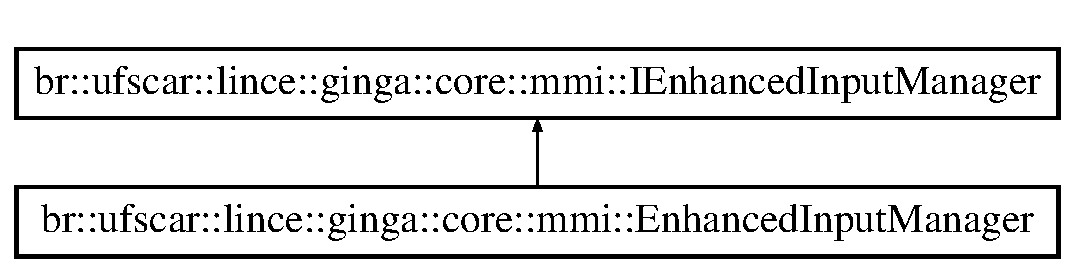
\includegraphics[height=2cm]{classbr_1_1ufscar_1_1lince_1_1ginga_1_1core_1_1mmi_1_1IEnhancedInputManager}
\end{center}
\end{figure}
\subsection*{Métodos Públicos}
\begin{DoxyCompactItemize}
\item 
virtual void {\bf addInputMode} (string inputModeName, {\bf IInputMode} $\ast$inputMode)=0
\item 
virtual {\bf IInputMode} $\ast$ {\bf removeInputMode} (string inputModeName)=0
\item 
virtual {\bf IInputMode} $\ast$ {\bf getInputMode} (string inputModeName)=0
\item 
virtual void {\bf gotoInputMode} (string inputModeName)=0
\item 
virtual void {\bf postMultimodalEvent} ({\bf IMultimodalInputEvent} $\ast$multimodalInputEvent)=0
\item 
virtual void {\bf addMultimodalInputEventListener} ({\bf IMultimodalInputEventListener} $\ast$listener)=0
\item 
virtual void {\bf removeMultimodalInputEventListener} ({\bf IMultimodalInputEventListener} $\ast$listener)=0
\item 
virtual int {\bf addCode} (string codeStr)=0
\item 
virtual bool {\bf removeCode} (int code)=0
\item 
virtual bool {\bf removeCode} (string codeStr)=0
\item 
virtual bool {\bf hasCode} (int code)=0
\item 
virtual bool {\bf hasCode} (string codeStr)=0
\item 
virtual void {\bf postMultimodalEvent} (string xml)=0
\item 
virtual void {\bf waitForUnlockCondition} ()=0
\end{DoxyCompactItemize}


\subsection{Descrição Detalhada}
Interface do gerenciador de eventos estendido para dar suporte a eventos multimodais. 

\subsection{Métodos}
\index{br::ufscar::lince::ginga::core::mmi::IEnhancedInputManager@{br::ufscar::lince::ginga::core::mmi::IEnhancedInputManager}!addCode@{addCode}}
\index{addCode@{addCode}!br::ufscar::lince::ginga::core::mmi::IEnhancedInputManager@{br::ufscar::lince::ginga::core::mmi::IEnhancedInputManager}}
\subsubsection[{addCode}]{\setlength{\rightskip}{0pt plus 5cm}virtual int br::ufscar::lince::ginga::core::mmi::IEnhancedInputManager::addCode (string {\em codeStr})\hspace{0.3cm}{\ttfamily  [pure virtual]}}\label{classbr_1_1ufscar_1_1lince_1_1ginga_1_1core_1_1mmi_1_1IEnhancedInputManager_abd69b86a5205125e16ff3498f9fbcc6e}
Adiciona um novo código de tecla. 
\begin{DoxyParams}{Parâmetros}
\item[{\em codeStr}]Identificador da nova tecla. \end{DoxyParams}
\begin{DoxyReturn}{Retorna}
Código atribuido à tecla. 
\end{DoxyReturn}


Implementado por {\bf br::ufscar::lince::ginga::core::mmi::EnhancedInputManager} \doxyref{}{pag.}{classbr_1_1ufscar_1_1lince_1_1ginga_1_1core_1_1mmi_1_1EnhancedInputManager_ae712d436ac1e9a101ac83051905db21b}.

\index{br::ufscar::lince::ginga::core::mmi::IEnhancedInputManager@{br::ufscar::lince::ginga::core::mmi::IEnhancedInputManager}!addInputMode@{addInputMode}}
\index{addInputMode@{addInputMode}!br::ufscar::lince::ginga::core::mmi::IEnhancedInputManager@{br::ufscar::lince::ginga::core::mmi::IEnhancedInputManager}}
\subsubsection[{addInputMode}]{\setlength{\rightskip}{0pt plus 5cm}virtual void br::ufscar::lince::ginga::core::mmi::IEnhancedInputManager::addInputMode (string {\em inputModeName}, \/  {\bf IInputMode} $\ast$ {\em inputMode})\hspace{0.3cm}{\ttfamily  [pure virtual]}}\label{classbr_1_1ufscar_1_1lince_1_1ginga_1_1core_1_1mmi_1_1IEnhancedInputManager_ac3620e81bb403ee7468de5752095ac0a}
Adicina um novo modo de entrada. 
\begin{DoxyParams}{Parâmetros}
\item[{\em inputModeName}]Nome do novo modo de entrada. \item[{\em inputMode}]Novo modo de entrada. \end{DoxyParams}

\begin{DoxyExceptions}{Exceções}
\item[{\em BadArgumentException}]se inputMode for nulo. \item[{\em \doxyref{DuplicateException}{pag.}{classbr_1_1ufscar_1_1lince_1_1ginga_1_1core_1_1mmi_1_1DuplicateException}}]se outro modo já adicionado possuir inputModeName como identificador. \end{DoxyExceptions}


Implementado por {\bf br::ufscar::lince::ginga::core::mmi::EnhancedInputManager} \doxyref{}{pag.}{classbr_1_1ufscar_1_1lince_1_1ginga_1_1core_1_1mmi_1_1EnhancedInputManager_a9f2d1868f1a67f2f51e1df07484d5be1}.

\index{br::ufscar::lince::ginga::core::mmi::IEnhancedInputManager@{br::ufscar::lince::ginga::core::mmi::IEnhancedInputManager}!addMultimodalInputEventListener@{addMultimodalInputEventListener}}
\index{addMultimodalInputEventListener@{addMultimodalInputEventListener}!br::ufscar::lince::ginga::core::mmi::IEnhancedInputManager@{br::ufscar::lince::ginga::core::mmi::IEnhancedInputManager}}
\subsubsection[{addMultimodalInputEventListener}]{\setlength{\rightskip}{0pt plus 5cm}virtual void br::ufscar::lince::ginga::core::mmi::IEnhancedInputManager::addMultimodalInputEventListener ({\bf IMultimodalInputEventListener} $\ast$ {\em listener})\hspace{0.3cm}{\ttfamily  [pure virtual]}}\label{classbr_1_1ufscar_1_1lince_1_1ginga_1_1core_1_1mmi_1_1IEnhancedInputManager_a5be22768c393249571ded39e79ed8dda}
Registra um observador de eventos multimodais. 
\begin{DoxyParams}{Parâmetros}
\item[{\em listener}]O observador a ser registrado. \end{DoxyParams}


Implementado por {\bf br::ufscar::lince::ginga::core::mmi::EnhancedInputManager} \doxyref{}{pag.}{classbr_1_1ufscar_1_1lince_1_1ginga_1_1core_1_1mmi_1_1EnhancedInputManager_af2f533b4ca43c0df2f712ef04183d166}.

\index{br::ufscar::lince::ginga::core::mmi::IEnhancedInputManager@{br::ufscar::lince::ginga::core::mmi::IEnhancedInputManager}!getInputMode@{getInputMode}}
\index{getInputMode@{getInputMode}!br::ufscar::lince::ginga::core::mmi::IEnhancedInputManager@{br::ufscar::lince::ginga::core::mmi::IEnhancedInputManager}}
\subsubsection[{getInputMode}]{\setlength{\rightskip}{0pt plus 5cm}virtual {\bf IInputMode}$\ast$ br::ufscar::lince::ginga::core::mmi::IEnhancedInputManager::getInputMode (string {\em inputModeName})\hspace{0.3cm}{\ttfamily  [pure virtual]}}\label{classbr_1_1ufscar_1_1lince_1_1ginga_1_1core_1_1mmi_1_1IEnhancedInputManager_acef61e560c6a3576d4530ce6c8db125a}
Acessa um modo de entrada previamente adicionado. 
\begin{DoxyParams}{Parâmetros}
\item[{\em inputModeName}]Nome do modo de entrada a ser acessado. \end{DoxyParams}
\begin{DoxyReturn}{Retorna}
O modo de entrada ou NULL caso o modo não seja encontrado. 
\end{DoxyReturn}


Implementado por {\bf br::ufscar::lince::ginga::core::mmi::EnhancedInputManager} \doxyref{}{pag.}{classbr_1_1ufscar_1_1lince_1_1ginga_1_1core_1_1mmi_1_1EnhancedInputManager_a6d3cd7e5533be32dc80f1f8659bd5920}.

\index{br::ufscar::lince::ginga::core::mmi::IEnhancedInputManager@{br::ufscar::lince::ginga::core::mmi::IEnhancedInputManager}!gotoInputMode@{gotoInputMode}}
\index{gotoInputMode@{gotoInputMode}!br::ufscar::lince::ginga::core::mmi::IEnhancedInputManager@{br::ufscar::lince::ginga::core::mmi::IEnhancedInputManager}}
\subsubsection[{gotoInputMode}]{\setlength{\rightskip}{0pt plus 5cm}virtual void br::ufscar::lince::ginga::core::mmi::IEnhancedInputManager::gotoInputMode (string {\em inputModeName})\hspace{0.3cm}{\ttfamily  [pure virtual]}}\label{classbr_1_1ufscar_1_1lince_1_1ginga_1_1core_1_1mmi_1_1IEnhancedInputManager_a09a9c5af4124bc571515e94f68b07256}
Atvia um modo de entrada previamente adicionado. 
\begin{DoxyParams}{Parâmetros}
\item[{\em inputModeName}]Nome do modo de entrada a ser ativado. \end{DoxyParams}


Implementado por {\bf br::ufscar::lince::ginga::core::mmi::EnhancedInputManager} \doxyref{}{pag.}{classbr_1_1ufscar_1_1lince_1_1ginga_1_1core_1_1mmi_1_1EnhancedInputManager_a516c9e18cabe5b1daab04c5fd73d5eaa}.

\index{br::ufscar::lince::ginga::core::mmi::IEnhancedInputManager@{br::ufscar::lince::ginga::core::mmi::IEnhancedInputManager}!hasCode@{hasCode}}
\index{hasCode@{hasCode}!br::ufscar::lince::ginga::core::mmi::IEnhancedInputManager@{br::ufscar::lince::ginga::core::mmi::IEnhancedInputManager}}
\subsubsection[{hasCode}]{\setlength{\rightskip}{0pt plus 5cm}virtual bool br::ufscar::lince::ginga::core::mmi::IEnhancedInputManager::hasCode (string {\em codeStr})\hspace{0.3cm}{\ttfamily  [pure virtual]}}\label{classbr_1_1ufscar_1_1lince_1_1ginga_1_1core_1_1mmi_1_1IEnhancedInputManager_a1d998e5010e297c48ae13fc47c9c5234}
Verifica se uma dada tecla existe no conjunto de teclas mapeadas. 
\begin{DoxyParams}{Parâmetros}
\item[{\em codeStr}]Identificador da tecla a ser chegada. \end{DoxyParams}
\begin{DoxyReturn}{Retorna}
true se a tecla existir; false caso contrário. 
\end{DoxyReturn}


Implementado por {\bf br::ufscar::lince::ginga::core::mmi::EnhancedInputManager} \doxyref{}{pag.}{classbr_1_1ufscar_1_1lince_1_1ginga_1_1core_1_1mmi_1_1EnhancedInputManager_a2e66b0f723f9abb5f9589f56d1e21d75}.

\index{br::ufscar::lince::ginga::core::mmi::IEnhancedInputManager@{br::ufscar::lince::ginga::core::mmi::IEnhancedInputManager}!hasCode@{hasCode}}
\index{hasCode@{hasCode}!br::ufscar::lince::ginga::core::mmi::IEnhancedInputManager@{br::ufscar::lince::ginga::core::mmi::IEnhancedInputManager}}
\subsubsection[{hasCode}]{\setlength{\rightskip}{0pt plus 5cm}virtual bool br::ufscar::lince::ginga::core::mmi::IEnhancedInputManager::hasCode (int {\em code})\hspace{0.3cm}{\ttfamily  [pure virtual]}}\label{classbr_1_1ufscar_1_1lince_1_1ginga_1_1core_1_1mmi_1_1IEnhancedInputManager_ad60eb6cadce0c06f8b1ac07528635d0c}
Verifica se uma dada tecla existe no conjunto de teclas mapeadas. 
\begin{DoxyParams}{Parâmetros}
\item[{\em code}]Código da tecla a ser chegada. \end{DoxyParams}
\begin{DoxyReturn}{Retorna}
true se a tecla existir; false caso contrário. 
\end{DoxyReturn}


Implementado por {\bf br::ufscar::lince::ginga::core::mmi::EnhancedInputManager} \doxyref{}{pag.}{classbr_1_1ufscar_1_1lince_1_1ginga_1_1core_1_1mmi_1_1EnhancedInputManager_a41b5236e73086da4ad199087f00f7b5b}.

\index{br::ufscar::lince::ginga::core::mmi::IEnhancedInputManager@{br::ufscar::lince::ginga::core::mmi::IEnhancedInputManager}!postMultimodalEvent@{postMultimodalEvent}}
\index{postMultimodalEvent@{postMultimodalEvent}!br::ufscar::lince::ginga::core::mmi::IEnhancedInputManager@{br::ufscar::lince::ginga::core::mmi::IEnhancedInputManager}}
\subsubsection[{postMultimodalEvent}]{\setlength{\rightskip}{0pt plus 5cm}virtual void br::ufscar::lince::ginga::core::mmi::IEnhancedInputManager::postMultimodalEvent (string {\em xml})\hspace{0.3cm}{\ttfamily  [pure virtual]}}\label{classbr_1_1ufscar_1_1lince_1_1ginga_1_1core_1_1mmi_1_1IEnhancedInputManager_a164d3b69f779481390962b44e2e30c3c}
Permite a notificação da chegada de um evento multimodal através do protocolo em xml. 
\begin{DoxyParams}{Parâmetros}
\item[{\em xml}]Conteúdo do xml representando o evento multimodal, ou caminho para o arquivo. Caso a string comece com o caracter '$<$', será considerado que trata-\/se do conteúdo, caso contrário, que trata-\/se do caminho para o arquivo. \end{DoxyParams}


Implementado por {\bf br::ufscar::lince::ginga::core::mmi::EnhancedInputManager} \doxyref{}{pag.}{classbr_1_1ufscar_1_1lince_1_1ginga_1_1core_1_1mmi_1_1EnhancedInputManager_ac54fd185c441d02b9a925c366c4de866}.

\index{br::ufscar::lince::ginga::core::mmi::IEnhancedInputManager@{br::ufscar::lince::ginga::core::mmi::IEnhancedInputManager}!postMultimodalEvent@{postMultimodalEvent}}
\index{postMultimodalEvent@{postMultimodalEvent}!br::ufscar::lince::ginga::core::mmi::IEnhancedInputManager@{br::ufscar::lince::ginga::core::mmi::IEnhancedInputManager}}
\subsubsection[{postMultimodalEvent}]{\setlength{\rightskip}{0pt plus 5cm}virtual void br::ufscar::lince::ginga::core::mmi::IEnhancedInputManager::postMultimodalEvent ({\bf IMultimodalInputEvent} $\ast$ {\em multimodalInputEvent})\hspace{0.3cm}{\ttfamily  [pure virtual]}}\label{classbr_1_1ufscar_1_1lince_1_1ginga_1_1core_1_1mmi_1_1IEnhancedInputManager_a1b294030cfc45c78836c05488f95582a}
Permite a notificação a ocorrência de um evento multimodal. 
\begin{DoxyParams}{Parâmetros}
\item[{\em multimodalInputEvent}]O evento multimodal ocorrido. \end{DoxyParams}


Implementado por {\bf br::ufscar::lince::ginga::core::mmi::EnhancedInputManager} \doxyref{}{pag.}{classbr_1_1ufscar_1_1lince_1_1ginga_1_1core_1_1mmi_1_1EnhancedInputManager_a6e2e28a5aa71bef5d112ad03219caa40}.

\index{br::ufscar::lince::ginga::core::mmi::IEnhancedInputManager@{br::ufscar::lince::ginga::core::mmi::IEnhancedInputManager}!removeCode@{removeCode}}
\index{removeCode@{removeCode}!br::ufscar::lince::ginga::core::mmi::IEnhancedInputManager@{br::ufscar::lince::ginga::core::mmi::IEnhancedInputManager}}
\subsubsection[{removeCode}]{\setlength{\rightskip}{0pt plus 5cm}virtual bool br::ufscar::lince::ginga::core::mmi::IEnhancedInputManager::removeCode (string {\em codeStr})\hspace{0.3cm}{\ttfamily  [pure virtual]}}\label{classbr_1_1ufscar_1_1lince_1_1ginga_1_1core_1_1mmi_1_1IEnhancedInputManager_a4d29e5e24c0a0fefbae57dee15113c53}
Remove uma tecla do conjunto de teclas mapeadas. 
\begin{DoxyParams}{Parâmetros}
\item[{\em codeStr}]Identificador a ser removida. \end{DoxyParams}
\begin{DoxyReturn}{Retorna}
true se a tecla foi removida com sucesso; false caso contrário. 
\end{DoxyReturn}


Implementado por {\bf br::ufscar::lince::ginga::core::mmi::EnhancedInputManager} \doxyref{}{pag.}{classbr_1_1ufscar_1_1lince_1_1ginga_1_1core_1_1mmi_1_1EnhancedInputManager_afe3a5063ea99cb766543c4a2c1054ec2}.

\index{br::ufscar::lince::ginga::core::mmi::IEnhancedInputManager@{br::ufscar::lince::ginga::core::mmi::IEnhancedInputManager}!removeCode@{removeCode}}
\index{removeCode@{removeCode}!br::ufscar::lince::ginga::core::mmi::IEnhancedInputManager@{br::ufscar::lince::ginga::core::mmi::IEnhancedInputManager}}
\subsubsection[{removeCode}]{\setlength{\rightskip}{0pt plus 5cm}virtual bool br::ufscar::lince::ginga::core::mmi::IEnhancedInputManager::removeCode (int {\em code})\hspace{0.3cm}{\ttfamily  [pure virtual]}}\label{classbr_1_1ufscar_1_1lince_1_1ginga_1_1core_1_1mmi_1_1IEnhancedInputManager_a7d16d1b63d954ebf7c29e75dd8ea60ec}
Remove uma tecla do conjunto de teclas mapeadas. 
\begin{DoxyParams}{Parâmetros}
\item[{\em code}]Código da tecla a ser removida. \end{DoxyParams}
\begin{DoxyReturn}{Retorna}
true se a tecla foi removida com sucesso; false caso contrário. 
\end{DoxyReturn}


Implementado por {\bf br::ufscar::lince::ginga::core::mmi::EnhancedInputManager} \doxyref{}{pag.}{classbr_1_1ufscar_1_1lince_1_1ginga_1_1core_1_1mmi_1_1EnhancedInputManager_a1d4a7473ddef29b2bd933293f8ed30b8}.

\index{br::ufscar::lince::ginga::core::mmi::IEnhancedInputManager@{br::ufscar::lince::ginga::core::mmi::IEnhancedInputManager}!removeInputMode@{removeInputMode}}
\index{removeInputMode@{removeInputMode}!br::ufscar::lince::ginga::core::mmi::IEnhancedInputManager@{br::ufscar::lince::ginga::core::mmi::IEnhancedInputManager}}
\subsubsection[{removeInputMode}]{\setlength{\rightskip}{0pt plus 5cm}virtual {\bf IInputMode}$\ast$ br::ufscar::lince::ginga::core::mmi::IEnhancedInputManager::removeInputMode (string {\em inputModeName})\hspace{0.3cm}{\ttfamily  [pure virtual]}}\label{classbr_1_1ufscar_1_1lince_1_1ginga_1_1core_1_1mmi_1_1IEnhancedInputManager_ad4b902e0a85aa2d0fe3df51d6b56f040}
Remove um modo de entrada previamente adicionado. 
\begin{DoxyParams}{Parâmetros}
\item[{\em inputModeName}]Nome do modo de entrada a ser removido. \end{DoxyParams}
\begin{DoxyReturn}{Retorna}
O modo de entrada removido ou NULL caso o modo não seja encontrado. 
\end{DoxyReturn}

\begin{DoxyExceptions}{Exceções}
\item[{\em BadArgumentException}]inputModeName for o identificador do modo de entrada atual. \end{DoxyExceptions}


Implementado por {\bf br::ufscar::lince::ginga::core::mmi::EnhancedInputManager} \doxyref{}{pag.}{classbr_1_1ufscar_1_1lince_1_1ginga_1_1core_1_1mmi_1_1EnhancedInputManager_ac8344e0a6779dff8ff9113482b39581b}.

\index{br::ufscar::lince::ginga::core::mmi::IEnhancedInputManager@{br::ufscar::lince::ginga::core::mmi::IEnhancedInputManager}!removeMultimodalInputEventListener@{removeMultimodalInputEventListener}}
\index{removeMultimodalInputEventListener@{removeMultimodalInputEventListener}!br::ufscar::lince::ginga::core::mmi::IEnhancedInputManager@{br::ufscar::lince::ginga::core::mmi::IEnhancedInputManager}}
\subsubsection[{removeMultimodalInputEventListener}]{\setlength{\rightskip}{0pt plus 5cm}virtual void br::ufscar::lince::ginga::core::mmi::IEnhancedInputManager::removeMultimodalInputEventListener ({\bf IMultimodalInputEventListener} $\ast$ {\em listener})\hspace{0.3cm}{\ttfamily  [pure virtual]}}\label{classbr_1_1ufscar_1_1lince_1_1ginga_1_1core_1_1mmi_1_1IEnhancedInputManager_a50eab137b503ba042f5e729c09433f71}
Remove um observador de eventos multimodais. 
\begin{DoxyParams}{Parâmetros}
\item[{\em listener}]O observador a ser removido. \end{DoxyParams}


Implementado por {\bf br::ufscar::lince::ginga::core::mmi::EnhancedInputManager} \doxyref{}{pag.}{classbr_1_1ufscar_1_1lince_1_1ginga_1_1core_1_1mmi_1_1EnhancedInputManager_abb4a1319555959cc0d4eae7cd8ff2459}.

\index{br::ufscar::lince::ginga::core::mmi::IEnhancedInputManager@{br::ufscar::lince::ginga::core::mmi::IEnhancedInputManager}!waitForUnlockCondition@{waitForUnlockCondition}}
\index{waitForUnlockCondition@{waitForUnlockCondition}!br::ufscar::lince::ginga::core::mmi::IEnhancedInputManager@{br::ufscar::lince::ginga::core::mmi::IEnhancedInputManager}}
\subsubsection[{waitForUnlockCondition}]{\setlength{\rightskip}{0pt plus 5cm}virtual void br::ufscar::lince::ginga::core::mmi::IEnhancedInputManager::waitForUnlockCondition ()\hspace{0.3cm}{\ttfamily  [pure virtual]}}\label{classbr_1_1ufscar_1_1lince_1_1ginga_1_1core_1_1mmi_1_1IEnhancedInputManager_a3a04932e36833d64ba65ef352bfdf7f5}
Para permitir que a main fique travada mesmo sem estar recebendo um fluxo de dados ou sem existir uma aplicação ncl rodando 

Implementado por {\bf br::ufscar::lince::ginga::core::mmi::EnhancedInputManager} \doxyref{}{pag.}{classbr_1_1ufscar_1_1lince_1_1ginga_1_1core_1_1mmi_1_1EnhancedInputManager_ab33e407205f97459c0ef0137b80d2eda}.



A documentação para esta classe foi gerada a partir do seguinte arquivo:\begin{DoxyCompactItemize}
\item 
include/{\bf IEnhancedInputManager.h}\end{DoxyCompactItemize}

\section{Referência da Classe br::ufscar::lince::ginga::core::mmi::IInputMode}
\label{classbr_1_1ufscar_1_1lince_1_1ginga_1_1core_1_1mmi_1_1IInputMode}\index{br::ufscar::lince::ginga::core::mmi::IInputMode@{br::ufscar::lince::ginga::core::mmi::IInputMode}}


{\ttfamily \#include $<$IInputMode.h$>$}

Diagrama de Hierarquia para br::ufscar::lince::ginga::core::mmi::IInputMode:\begin{figure}[H]
\begin{center}
\leavevmode
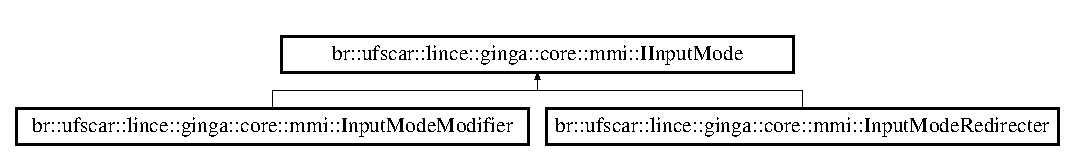
\includegraphics[height=1.71254cm]{classbr_1_1ufscar_1_1lince_1_1ginga_1_1core_1_1mmi_1_1IInputMode}
\end{center}
\end{figure}
\subsection*{Métodos Públicos}
\begin{DoxyCompactItemize}
\item 
virtual void {\bf startingInputMode} ()=0
\item 
virtual void {\bf exitingInputMode} ()=0
\item 
virtual void {\bf initializeInputMode} ()=0
\item 
virtual int {\bf getInputModeType} ()=0
\end{DoxyCompactItemize}
\subsection*{Atributos Estáticos Públicos}
\begin{DoxyCompactItemize}
\item 
static const int {\bf REDIRECTER} = 0\label{classbr_1_1ufscar_1_1lince_1_1ginga_1_1core_1_1mmi_1_1IInputMode_adfaf56966018115a16565ad04c02b926}

\begin{DoxyCompactList}\small\item\em Representa Modos de entrada redirecionadores de eventos. \item\end{DoxyCompactList}\item 
static const int {\bf MODIFIER} = 1\label{classbr_1_1ufscar_1_1lince_1_1ginga_1_1core_1_1mmi_1_1IInputMode_a8a2c52c5712a9ba699ddb0d8a61ed31c}

\begin{DoxyCompactList}\small\item\em Represente Modos de entrada modificadores de eventos. \item\end{DoxyCompactList}\end{DoxyCompactItemize}


\subsection{Descrição Detalhada}
Interface que representa um modo de entrada de eventos. Pode representar um redirecionador ou um modificador de eventos. 

\subsection{Métodos}
\index{br::ufscar::lince::ginga::core::mmi::IInputMode@{br::ufscar::lince::ginga::core::mmi::IInputMode}!exitingInputMode@{exitingInputMode}}
\index{exitingInputMode@{exitingInputMode}!br::ufscar::lince::ginga::core::mmi::IInputMode@{br::ufscar::lince::ginga::core::mmi::IInputMode}}
\subsubsection[{exitingInputMode}]{\setlength{\rightskip}{0pt plus 5cm}virtual void br::ufscar::lince::ginga::core::mmi::IInputMode::exitingInputMode ()\hspace{0.3cm}{\ttfamily  [pure virtual]}}\label{classbr_1_1ufscar_1_1lince_1_1ginga_1_1core_1_1mmi_1_1IInputMode_abf8a189982838fe77f481c9c62449e1b}
Método chamado quando o modo de entrada é desativado. 

Referenciado por br::ufscar::lince::ginga::core::mmi::EnhancedInputManager::nextInputMode().

\index{br::ufscar::lince::ginga::core::mmi::IInputMode@{br::ufscar::lince::ginga::core::mmi::IInputMode}!getInputModeType@{getInputModeType}}
\index{getInputModeType@{getInputModeType}!br::ufscar::lince::ginga::core::mmi::IInputMode@{br::ufscar::lince::ginga::core::mmi::IInputMode}}
\subsubsection[{getInputModeType}]{\setlength{\rightskip}{0pt plus 5cm}virtual int br::ufscar::lince::ginga::core::mmi::IInputMode::getInputModeType ()\hspace{0.3cm}{\ttfamily  [pure virtual]}}\label{classbr_1_1ufscar_1_1lince_1_1ginga_1_1core_1_1mmi_1_1IInputMode_a54f7e96cd446cf07e781cd07d55ae99a}
Retorna um constante inteira que representa o tipo de modo de entrada. \begin{DoxyReturn}{Retorna}
REDIRECTER se for um modo redirecionador; MODIFIER se for um modo modificador. 
\end{DoxyReturn}


Implementado por {\bf br::ufscar::lince::ginga::core::mmi::InputModeModifier} \doxyref{}{pag.}{classbr_1_1ufscar_1_1lince_1_1ginga_1_1core_1_1mmi_1_1InputModeModifier_a75a4129026ec1170e25defb04d00a1a3} e {\bf br::ufscar::lince::ginga::core::mmi::InputModeRedirecter} \doxyref{}{pag.}{classbr_1_1ufscar_1_1lince_1_1ginga_1_1core_1_1mmi_1_1InputModeRedirecter_a4ede0c5c135504bf4746d1a43b531114}.

\index{br::ufscar::lince::ginga::core::mmi::IInputMode@{br::ufscar::lince::ginga::core::mmi::IInputMode}!initializeInputMode@{initializeInputMode}}
\index{initializeInputMode@{initializeInputMode}!br::ufscar::lince::ginga::core::mmi::IInputMode@{br::ufscar::lince::ginga::core::mmi::IInputMode}}
\subsubsection[{initializeInputMode}]{\setlength{\rightskip}{0pt plus 5cm}virtual void br::ufscar::lince::ginga::core::mmi::IInputMode::initializeInputMode ()\hspace{0.3cm}{\ttfamily  [pure virtual]}}\label{classbr_1_1ufscar_1_1lince_1_1ginga_1_1core_1_1mmi_1_1IInputMode_aabbbe0164832ed9d5804cf184bb83dce}
Método chamado quando o modo de entrada é adicionado aos modos existentes. \index{br::ufscar::lince::ginga::core::mmi::IInputMode@{br::ufscar::lince::ginga::core::mmi::IInputMode}!startingInputMode@{startingInputMode}}
\index{startingInputMode@{startingInputMode}!br::ufscar::lince::ginga::core::mmi::IInputMode@{br::ufscar::lince::ginga::core::mmi::IInputMode}}
\subsubsection[{startingInputMode}]{\setlength{\rightskip}{0pt plus 5cm}virtual void br::ufscar::lince::ginga::core::mmi::IInputMode::startingInputMode ()\hspace{0.3cm}{\ttfamily  [pure virtual]}}\label{classbr_1_1ufscar_1_1lince_1_1ginga_1_1core_1_1mmi_1_1IInputMode_a69dafa4a349410d4ba1020bbf5c06d7b}
Método chamado quando o modo de entrada é ativado. 

Referenciado por br::ufscar::lince::ginga::core::mmi::EnhancedInputManager::nextInputMode().



A documentação para esta classe foi gerada a partir do seguinte arquivo:\begin{DoxyCompactItemize}
\item 
include/{\bf IInputMode.h}\end{DoxyCompactItemize}

\section{Referência da Classe br::ufscar::lince::ginga::core::mmi::IMultimodalInputEvent}
\label{classbr_1_1ufscar_1_1lince_1_1ginga_1_1core_1_1mmi_1_1IMultimodalInputEvent}\index{br::ufscar::lince::ginga::core::mmi::IMultimodalInputEvent@{br::ufscar::lince::ginga::core::mmi::IMultimodalInputEvent}}


{\ttfamily \#include $<$IMultimodalInputEvent.h$>$}

Diagrama de Hierarquia para br::ufscar::lince::ginga::core::mmi::IMultimodalInputEvent:\begin{figure}[H]
\begin{center}
\leavevmode
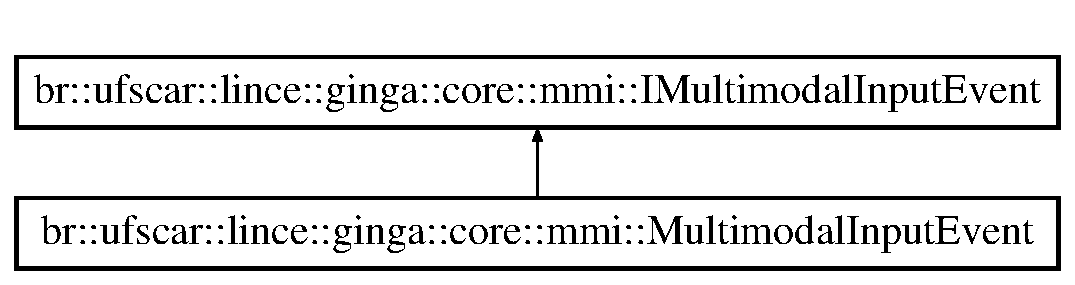
\includegraphics[height=2cm]{classbr_1_1ufscar_1_1lince_1_1ginga_1_1core_1_1mmi_1_1IMultimodalInputEvent}
\end{center}
\end{figure}
\subsection*{Métodos Públicos}
\begin{DoxyCompactItemize}
\item 
virtual {\bf $\sim$IMultimodalInputEvent} ()
\item 
virtual string {\bf getId} ()=0
\item 
virtual void {\bf setId} (string id)=0
\item 
virtual void {\bf addValue} (string name, void $\ast$value)=0
\item 
virtual bool {\bf removeValue} (string name)=0
\item 
virtual map$<$ string, void $\ast$ $>$ $\ast$ {\bf getMultimodalValuesMap} ()=0
\item 
virtual void {\bf setMultimodalValuesMap} (map$<$ string, void $\ast$ $>$ $\ast$map)=0
\item 
virtual vector$<$ string $>$ $\ast$ {\bf getStrings} ()=0
\item 
virtual void {\bf addString} (string str)=0
\item 
virtual Ink $\ast$ {\bf getInk} ()=0
\item 
virtual void {\bf setInk} (Ink $\ast$ink)=0
\item 
virtual {\bf Acceleration} $\ast$ {\bf getAcceleration} ()=0
\item 
virtual void {\bf setAcceleration} ({\bf Acceleration} $\ast$accel)=0
\item 
virtual vector$<$ {\bf File} $\ast$ $>$ $\ast$ {\bf getBinaries} ()=0
\item 
virtual void {\bf addFile} ({\bf File} $\ast$f)=0
\end{DoxyCompactItemize}


\subsection{Descrição Detalhada}
Interface que representa um evento multimodal. 

\subsection{Construtores \& Destrutores}
\index{br::ufscar::lince::ginga::core::mmi::IMultimodalInputEvent@{br::ufscar::lince::ginga::core::mmi::IMultimodalInputEvent}!$\sim$IMultimodalInputEvent@{$\sim$IMultimodalInputEvent}}
\index{$\sim$IMultimodalInputEvent@{$\sim$IMultimodalInputEvent}!br::ufscar::lince::ginga::core::mmi::IMultimodalInputEvent@{br::ufscar::lince::ginga::core::mmi::IMultimodalInputEvent}}
\subsubsection[{$\sim$IMultimodalInputEvent}]{\setlength{\rightskip}{0pt plus 5cm}virtual br::ufscar::lince::ginga::core::mmi::IMultimodalInputEvent::$\sim$IMultimodalInputEvent ()\hspace{0.3cm}{\ttfamily  [inline, virtual]}}\label{classbr_1_1ufscar_1_1lince_1_1ginga_1_1core_1_1mmi_1_1IMultimodalInputEvent_ab16904f9f3cc150797d9fb6988cb266d}
Destrói o \doxyref{IMultimodalInputEvent}{pag.}{classbr_1_1ufscar_1_1lince_1_1ginga_1_1core_1_1mmi_1_1IMultimodalInputEvent}. 

\subsection{Métodos}
\index{br::ufscar::lince::ginga::core::mmi::IMultimodalInputEvent@{br::ufscar::lince::ginga::core::mmi::IMultimodalInputEvent}!addFile@{addFile}}
\index{addFile@{addFile}!br::ufscar::lince::ginga::core::mmi::IMultimodalInputEvent@{br::ufscar::lince::ginga::core::mmi::IMultimodalInputEvent}}
\subsubsection[{addFile}]{\setlength{\rightskip}{0pt plus 5cm}virtual void br::ufscar::lince::ginga::core::mmi::IMultimodalInputEvent::addFile ({\bf File} $\ast$ {\em f})\hspace{0.3cm}{\ttfamily  [pure virtual]}}\label{classbr_1_1ufscar_1_1lince_1_1ginga_1_1core_1_1mmi_1_1IMultimodalInputEvent_a2202acece2c5b201899ef73a374cb53e}
Adiciona um arquivo ao evento multimodal. 
\begin{DoxyParams}{Parâmetros}
\item[{\em f}]Arquivo a ser adicionad no evento. \end{DoxyParams}


Implementado por {\bf br::ufscar::lince::ginga::core::mmi::MultimodalInputEvent} \doxyref{}{pag.}{classbr_1_1ufscar_1_1lince_1_1ginga_1_1core_1_1mmi_1_1MultimodalInputEvent_ab4d9eb64514f673c9092b4d70fc2bef8}.



Referenciado por br::ufscar::lince::ginga::core::mmi::EventParser::parseBody().

\index{br::ufscar::lince::ginga::core::mmi::IMultimodalInputEvent@{br::ufscar::lince::ginga::core::mmi::IMultimodalInputEvent}!addString@{addString}}
\index{addString@{addString}!br::ufscar::lince::ginga::core::mmi::IMultimodalInputEvent@{br::ufscar::lince::ginga::core::mmi::IMultimodalInputEvent}}
\subsubsection[{addString}]{\setlength{\rightskip}{0pt plus 5cm}virtual void br::ufscar::lince::ginga::core::mmi::IMultimodalInputEvent::addString (string {\em str})\hspace{0.3cm}{\ttfamily  [pure virtual]}}\label{classbr_1_1ufscar_1_1lince_1_1ginga_1_1core_1_1mmi_1_1IMultimodalInputEvent_a17f4a388d7854789b10d68615b098d56}
Adiciona uma string ao evento multimodal. 
\begin{DoxyParams}{Parâmetros}
\item[{\em str}]String a ser adicionada no evento. \end{DoxyParams}


Implementado por {\bf br::ufscar::lince::ginga::core::mmi::MultimodalInputEvent} \doxyref{}{pag.}{classbr_1_1ufscar_1_1lince_1_1ginga_1_1core_1_1mmi_1_1MultimodalInputEvent_af375eab32140b0faa2f860feee4c5870}.



Referenciado por br::ufscar::lince::ginga::core::mmi::EventParser::parseBody().

\index{br::ufscar::lince::ginga::core::mmi::IMultimodalInputEvent@{br::ufscar::lince::ginga::core::mmi::IMultimodalInputEvent}!addValue@{addValue}}
\index{addValue@{addValue}!br::ufscar::lince::ginga::core::mmi::IMultimodalInputEvent@{br::ufscar::lince::ginga::core::mmi::IMultimodalInputEvent}}
\subsubsection[{addValue}]{\setlength{\rightskip}{0pt plus 5cm}virtual void br::ufscar::lince::ginga::core::mmi::IMultimodalInputEvent::addValue (string {\em name}, \/  void $\ast$ {\em value})\hspace{0.3cm}{\ttfamily  [pure virtual]}}\label{classbr_1_1ufscar_1_1lince_1_1ginga_1_1core_1_1mmi_1_1IMultimodalInputEvent_ad10863e1dbfe978e89729ad629edb815}
Adiciona um valor ao evento multimodal. 
\begin{DoxyParams}{Parâmetros}
\item[{\em name}]do valor a ser adicionado. \item[{\em value}]conteúdo do valor a ser adicionado. \end{DoxyParams}


Implementado por {\bf br::ufscar::lince::ginga::core::mmi::MultimodalInputEvent} \doxyref{}{pag.}{classbr_1_1ufscar_1_1lince_1_1ginga_1_1core_1_1mmi_1_1MultimodalInputEvent_a35451b8fa11bb048860f738268bfdf1c}.



Referenciado por br::ufscar::lince::ginga::core::mmi::EventParser::parseBody() e br::ufscar::lince::ginga::core::mmi::EventParser::parseHead().

\index{br::ufscar::lince::ginga::core::mmi::IMultimodalInputEvent@{br::ufscar::lince::ginga::core::mmi::IMultimodalInputEvent}!getAcceleration@{getAcceleration}}
\index{getAcceleration@{getAcceleration}!br::ufscar::lince::ginga::core::mmi::IMultimodalInputEvent@{br::ufscar::lince::ginga::core::mmi::IMultimodalInputEvent}}
\subsubsection[{getAcceleration}]{\setlength{\rightskip}{0pt plus 5cm}virtual {\bf Acceleration}$\ast$ br::ufscar::lince::ginga::core::mmi::IMultimodalInputEvent::getAcceleration ()\hspace{0.3cm}{\ttfamily  [pure virtual]}}\label{classbr_1_1ufscar_1_1lince_1_1ginga_1_1core_1_1mmi_1_1IMultimodalInputEvent_a9ed35bcbcbb3cbb20b050d5665d9ff35}
Acessa o objeto acceleration do evento multimodal. \begin{DoxyReturn}{Retorna}
objeto \doxyref{Acceleration}{pag.}{classbr_1_1ufscar_1_1lince_1_1ginga_1_1core_1_1mmi_1_1Acceleration} com os dados de aceleração do evento. 
\end{DoxyReturn}


Implementado por {\bf br::ufscar::lince::ginga::core::mmi::MultimodalInputEvent} \doxyref{}{pag.}{classbr_1_1ufscar_1_1lince_1_1ginga_1_1core_1_1mmi_1_1MultimodalInputEvent_ada47dfbfd8048f03f96c336ef4f9ec75}.

\index{br::ufscar::lince::ginga::core::mmi::IMultimodalInputEvent@{br::ufscar::lince::ginga::core::mmi::IMultimodalInputEvent}!getBinaries@{getBinaries}}
\index{getBinaries@{getBinaries}!br::ufscar::lince::ginga::core::mmi::IMultimodalInputEvent@{br::ufscar::lince::ginga::core::mmi::IMultimodalInputEvent}}
\subsubsection[{getBinaries}]{\setlength{\rightskip}{0pt plus 5cm}virtual vector$<${\bf File}$\ast$$>$$\ast$ br::ufscar::lince::ginga::core::mmi::IMultimodalInputEvent::getBinaries ()\hspace{0.3cm}{\ttfamily  [pure virtual]}}\label{classbr_1_1ufscar_1_1lince_1_1ginga_1_1core_1_1mmi_1_1IMultimodalInputEvent_a3616b43630e332773c482d6406c00a2f}
Acessa os arquivos do evento multimodal. \begin{DoxyReturn}{Retorna}
vetor de arquivos. 
\end{DoxyReturn}


Implementado por {\bf br::ufscar::lince::ginga::core::mmi::MultimodalInputEvent} \doxyref{}{pag.}{classbr_1_1ufscar_1_1lince_1_1ginga_1_1core_1_1mmi_1_1MultimodalInputEvent_a4abcfcedec49098c0279db3097433f29}.

\index{br::ufscar::lince::ginga::core::mmi::IMultimodalInputEvent@{br::ufscar::lince::ginga::core::mmi::IMultimodalInputEvent}!getId@{getId}}
\index{getId@{getId}!br::ufscar::lince::ginga::core::mmi::IMultimodalInputEvent@{br::ufscar::lince::ginga::core::mmi::IMultimodalInputEvent}}
\subsubsection[{getId}]{\setlength{\rightskip}{0pt plus 5cm}virtual string br::ufscar::lince::ginga::core::mmi::IMultimodalInputEvent::getId ()\hspace{0.3cm}{\ttfamily  [pure virtual]}}\label{classbr_1_1ufscar_1_1lince_1_1ginga_1_1core_1_1mmi_1_1IMultimodalInputEvent_a61a42387f2e29c30639905079695d8f8}
Acessa o id do evento multimodal. \begin{DoxyReturn}{Retorna}
id do evento. 
\end{DoxyReturn}


Implementado por {\bf br::ufscar::lince::ginga::core::mmi::MultimodalInputEvent} \doxyref{}{pag.}{classbr_1_1ufscar_1_1lince_1_1ginga_1_1core_1_1mmi_1_1MultimodalInputEvent_a1a6648f772f8ae29244dbfccd61c1e61}.



Referenciado por br::ufscar::lince::ginga::core::mmi::EnhancedInputManager::postMultimodalEvent().

\index{br::ufscar::lince::ginga::core::mmi::IMultimodalInputEvent@{br::ufscar::lince::ginga::core::mmi::IMultimodalInputEvent}!getInk@{getInk}}
\index{getInk@{getInk}!br::ufscar::lince::ginga::core::mmi::IMultimodalInputEvent@{br::ufscar::lince::ginga::core::mmi::IMultimodalInputEvent}}
\subsubsection[{getInk}]{\setlength{\rightskip}{0pt plus 5cm}virtual Ink$\ast$ br::ufscar::lince::ginga::core::mmi::IMultimodalInputEvent::getInk ()\hspace{0.3cm}{\ttfamily  [pure virtual]}}\label{classbr_1_1ufscar_1_1lince_1_1ginga_1_1core_1_1mmi_1_1IMultimodalInputEvent_a23a24cc399ceb022a43a60c46ae6a6d9}
Acessa o objeto ink do evento multimodal. \begin{DoxyReturn}{Retorna}
Objeto com os dados de tinta do evento. 
\end{DoxyReturn}


Implementado por {\bf br::ufscar::lince::ginga::core::mmi::MultimodalInputEvent} \doxyref{}{pag.}{classbr_1_1ufscar_1_1lince_1_1ginga_1_1core_1_1mmi_1_1MultimodalInputEvent_ac1dcabf82763009c60dfc3c63c43ec1a}.

\index{br::ufscar::lince::ginga::core::mmi::IMultimodalInputEvent@{br::ufscar::lince::ginga::core::mmi::IMultimodalInputEvent}!getMultimodalValuesMap@{getMultimodalValuesMap}}
\index{getMultimodalValuesMap@{getMultimodalValuesMap}!br::ufscar::lince::ginga::core::mmi::IMultimodalInputEvent@{br::ufscar::lince::ginga::core::mmi::IMultimodalInputEvent}}
\subsubsection[{getMultimodalValuesMap}]{\setlength{\rightskip}{0pt plus 5cm}virtual map$<$string, void$\ast$$>$$\ast$ br::ufscar::lince::ginga::core::mmi::IMultimodalInputEvent::getMultimodalValuesMap ()\hspace{0.3cm}{\ttfamily  [pure virtual]}}\label{classbr_1_1ufscar_1_1lince_1_1ginga_1_1core_1_1mmi_1_1IMultimodalInputEvent_a2063d0a8661ed4e178bab240c91cc014}
Acessa os valores contidos no evento multimodal. \begin{DoxyReturn}{Retorna}
mapa com os pares nome,valor do evento multimodal. 
\end{DoxyReturn}


Implementado por {\bf br::ufscar::lince::ginga::core::mmi::MultimodalInputEvent} \doxyref{}{pag.}{classbr_1_1ufscar_1_1lince_1_1ginga_1_1core_1_1mmi_1_1MultimodalInputEvent_abafe975af04a1680cc8184fcba8de6a4}.

\index{br::ufscar::lince::ginga::core::mmi::IMultimodalInputEvent@{br::ufscar::lince::ginga::core::mmi::IMultimodalInputEvent}!getStrings@{getStrings}}
\index{getStrings@{getStrings}!br::ufscar::lince::ginga::core::mmi::IMultimodalInputEvent@{br::ufscar::lince::ginga::core::mmi::IMultimodalInputEvent}}
\subsubsection[{getStrings}]{\setlength{\rightskip}{0pt plus 5cm}virtual vector$<$string$>$$\ast$ br::ufscar::lince::ginga::core::mmi::IMultimodalInputEvent::getStrings ()\hspace{0.3cm}{\ttfamily  [pure virtual]}}\label{classbr_1_1ufscar_1_1lince_1_1ginga_1_1core_1_1mmi_1_1IMultimodalInputEvent_a41a14202b17c64e7d0216d47bfeebfd9}
Acessa as strings do evento multimodal. \begin{DoxyReturn}{Retorna}
vetor de strings. 
\end{DoxyReturn}


Implementado por {\bf br::ufscar::lince::ginga::core::mmi::MultimodalInputEvent} \doxyref{}{pag.}{classbr_1_1ufscar_1_1lince_1_1ginga_1_1core_1_1mmi_1_1MultimodalInputEvent_ae9a66008d133d84eb977dad43b379ae5}.

\index{br::ufscar::lince::ginga::core::mmi::IMultimodalInputEvent@{br::ufscar::lince::ginga::core::mmi::IMultimodalInputEvent}!removeValue@{removeValue}}
\index{removeValue@{removeValue}!br::ufscar::lince::ginga::core::mmi::IMultimodalInputEvent@{br::ufscar::lince::ginga::core::mmi::IMultimodalInputEvent}}
\subsubsection[{removeValue}]{\setlength{\rightskip}{0pt plus 5cm}virtual bool br::ufscar::lince::ginga::core::mmi::IMultimodalInputEvent::removeValue (string {\em name})\hspace{0.3cm}{\ttfamily  [pure virtual]}}\label{classbr_1_1ufscar_1_1lince_1_1ginga_1_1core_1_1mmi_1_1IMultimodalInputEvent_adfcffaf158db42a0d0fb6e522faad91f}
Remove um valor do evento multimodal. 
\begin{DoxyParams}{Parâmetros}
\item[{\em name}]Nome do valor a ser removido. \end{DoxyParams}
\begin{DoxyReturn}{Retorna}
true caso o valor tenha sido removido. 

false caso o valor não tenha sido removido. 
\end{DoxyReturn}


Implementado por {\bf br::ufscar::lince::ginga::core::mmi::MultimodalInputEvent} \doxyref{}{pag.}{classbr_1_1ufscar_1_1lince_1_1ginga_1_1core_1_1mmi_1_1MultimodalInputEvent_acb330a03e341bbf051aaf2a44c640b86}.

\index{br::ufscar::lince::ginga::core::mmi::IMultimodalInputEvent@{br::ufscar::lince::ginga::core::mmi::IMultimodalInputEvent}!setAcceleration@{setAcceleration}}
\index{setAcceleration@{setAcceleration}!br::ufscar::lince::ginga::core::mmi::IMultimodalInputEvent@{br::ufscar::lince::ginga::core::mmi::IMultimodalInputEvent}}
\subsubsection[{setAcceleration}]{\setlength{\rightskip}{0pt plus 5cm}virtual void br::ufscar::lince::ginga::core::mmi::IMultimodalInputEvent::setAcceleration ({\bf Acceleration} $\ast$ {\em accel})\hspace{0.3cm}{\ttfamily  [pure virtual]}}\label{classbr_1_1ufscar_1_1lince_1_1ginga_1_1core_1_1mmi_1_1IMultimodalInputEvent_a9ba0b45f1919bbfbe08bc0267a7452eb}
Define o objeto acceleration do evento multimodal. 
\begin{DoxyParams}{Parâmetros}
\item[{\em accel}]objeto com os dados de aceleração do evento. \end{DoxyParams}


Implementado por {\bf br::ufscar::lince::ginga::core::mmi::MultimodalInputEvent} \doxyref{}{pag.}{classbr_1_1ufscar_1_1lince_1_1ginga_1_1core_1_1mmi_1_1MultimodalInputEvent_a5f9638fa3fc331ab11e1aca30bc33035}.



Referenciado por br::ufscar::lince::ginga::core::mmi::EventParser::parseBody().

\index{br::ufscar::lince::ginga::core::mmi::IMultimodalInputEvent@{br::ufscar::lince::ginga::core::mmi::IMultimodalInputEvent}!setId@{setId}}
\index{setId@{setId}!br::ufscar::lince::ginga::core::mmi::IMultimodalInputEvent@{br::ufscar::lince::ginga::core::mmi::IMultimodalInputEvent}}
\subsubsection[{setId}]{\setlength{\rightskip}{0pt plus 5cm}virtual void br::ufscar::lince::ginga::core::mmi::IMultimodalInputEvent::setId (string {\em id})\hspace{0.3cm}{\ttfamily  [pure virtual]}}\label{classbr_1_1ufscar_1_1lince_1_1ginga_1_1core_1_1mmi_1_1IMultimodalInputEvent_aaaa1d0a0d5d196e2b3e43573404f2cca}
Define o id do evento multimodal. 
\begin{DoxyParams}{Parâmetros}
\item[{\em id}]do evento. \end{DoxyParams}


Implementado por {\bf br::ufscar::lince::ginga::core::mmi::MultimodalInputEvent} \doxyref{}{pag.}{classbr_1_1ufscar_1_1lince_1_1ginga_1_1core_1_1mmi_1_1MultimodalInputEvent_a5de98758c900a1523f3b52310c59b056}.

\index{br::ufscar::lince::ginga::core::mmi::IMultimodalInputEvent@{br::ufscar::lince::ginga::core::mmi::IMultimodalInputEvent}!setInk@{setInk}}
\index{setInk@{setInk}!br::ufscar::lince::ginga::core::mmi::IMultimodalInputEvent@{br::ufscar::lince::ginga::core::mmi::IMultimodalInputEvent}}
\subsubsection[{setInk}]{\setlength{\rightskip}{0pt plus 5cm}virtual void br::ufscar::lince::ginga::core::mmi::IMultimodalInputEvent::setInk (Ink $\ast$ {\em ink})\hspace{0.3cm}{\ttfamily  [pure virtual]}}\label{classbr_1_1ufscar_1_1lince_1_1ginga_1_1core_1_1mmi_1_1IMultimodalInputEvent_a2d7da14262a0127f188f69a72ec4a5de}
Define o objeto ink do evento multimodal. 
\begin{DoxyParams}{Parâmetros}
\item[{\em ink}]objeto com os dados de tinta do evento. \end{DoxyParams}


Implementado por {\bf br::ufscar::lince::ginga::core::mmi::MultimodalInputEvent} \doxyref{}{pag.}{classbr_1_1ufscar_1_1lince_1_1ginga_1_1core_1_1mmi_1_1MultimodalInputEvent_aa5b3575f54367657785e5dbae5139646}.



Referenciado por br::ufscar::lince::ginga::core::mmi::EventParser::parseBody().

\index{br::ufscar::lince::ginga::core::mmi::IMultimodalInputEvent@{br::ufscar::lince::ginga::core::mmi::IMultimodalInputEvent}!setMultimodalValuesMap@{setMultimodalValuesMap}}
\index{setMultimodalValuesMap@{setMultimodalValuesMap}!br::ufscar::lince::ginga::core::mmi::IMultimodalInputEvent@{br::ufscar::lince::ginga::core::mmi::IMultimodalInputEvent}}
\subsubsection[{setMultimodalValuesMap}]{\setlength{\rightskip}{0pt plus 5cm}virtual void br::ufscar::lince::ginga::core::mmi::IMultimodalInputEvent::setMultimodalValuesMap (map$<$ string, void $\ast$ $>$ $\ast$ {\em map})\hspace{0.3cm}{\ttfamily  [pure virtual]}}\label{classbr_1_1ufscar_1_1lince_1_1ginga_1_1core_1_1mmi_1_1IMultimodalInputEvent_ac9d69cb5bae636bf164d620dfb8c5d75}
Define os valores contidos dentro do evento multimodal. 
\begin{DoxyParams}{Parâmetros}
\item[{\em map}]Mapa com o par $<$nome,valor$>$. \end{DoxyParams}


Implementado por {\bf br::ufscar::lince::ginga::core::mmi::MultimodalInputEvent} \doxyref{}{pag.}{classbr_1_1ufscar_1_1lince_1_1ginga_1_1core_1_1mmi_1_1MultimodalInputEvent_a1d8c120f0c93b3ada06e6c3c165b0aea}.



A documentação para esta classe foi gerada a partir do seguinte arquivo:\begin{DoxyCompactItemize}
\item 
include/{\bf IMultimodalInputEvent.h}\end{DoxyCompactItemize}

\section{Referência da Classe br::ufscar::lince::ginga::core::mmi::IMultimodalInputEventListener}
\label{classbr_1_1ufscar_1_1lince_1_1ginga_1_1core_1_1mmi_1_1IMultimodalInputEventListener}\index{br::ufscar::lince::ginga::core::mmi::IMultimodalInputEventListener@{br::ufscar::lince::ginga::core::mmi::IMultimodalInputEventListener}}


{\ttfamily \#include $<$IMultimodalInputEventListener.h$>$}

\subsection*{Métodos Públicos}
\begin{DoxyCompactItemize}
\item 
virtual {\bf $\sim$IMultimodalInputEventListener} ()
\item 
virtual bool {\bf multimodalUserEventReceived} ({\bf IMultimodalInputEvent} $\ast$ev)=0
\end{DoxyCompactItemize}


\subsection{Descrição Detalhada}
Interface que representa um observador de eventos multimodais. 

\subsection{Construtores \& Destrutores}
\index{br::ufscar::lince::ginga::core::mmi::IMultimodalInputEventListener@{br::ufscar::lince::ginga::core::mmi::IMultimodalInputEventListener}!$\sim$IMultimodalInputEventListener@{$\sim$IMultimodalInputEventListener}}
\index{$\sim$IMultimodalInputEventListener@{$\sim$IMultimodalInputEventListener}!br::ufscar::lince::ginga::core::mmi::IMultimodalInputEventListener@{br::ufscar::lince::ginga::core::mmi::IMultimodalInputEventListener}}
\subsubsection[{$\sim$IMultimodalInputEventListener}]{\setlength{\rightskip}{0pt plus 5cm}virtual br::ufscar::lince::ginga::core::mmi::IMultimodalInputEventListener::$\sim$IMultimodalInputEventListener ()\hspace{0.3cm}{\ttfamily  [inline, virtual]}}\label{classbr_1_1ufscar_1_1lince_1_1ginga_1_1core_1_1mmi_1_1IMultimodalInputEventListener_a3a4390e4cfdb64cd46900284ad839a82}
Destrói o \doxyref{IMultimodalInputEventListener}{pag.}{classbr_1_1ufscar_1_1lince_1_1ginga_1_1core_1_1mmi_1_1IMultimodalInputEventListener}. 

\subsection{Métodos}
\index{br::ufscar::lince::ginga::core::mmi::IMultimodalInputEventListener@{br::ufscar::lince::ginga::core::mmi::IMultimodalInputEventListener}!multimodalUserEventReceived@{multimodalUserEventReceived}}
\index{multimodalUserEventReceived@{multimodalUserEventReceived}!br::ufscar::lince::ginga::core::mmi::IMultimodalInputEventListener@{br::ufscar::lince::ginga::core::mmi::IMultimodalInputEventListener}}
\subsubsection[{multimodalUserEventReceived}]{\setlength{\rightskip}{0pt plus 5cm}virtual bool br::ufscar::lince::ginga::core::mmi::IMultimodalInputEventListener::multimodalUserEventReceived ({\bf IMultimodalInputEvent} $\ast$ {\em ev})\hspace{0.3cm}{\ttfamily  [pure virtual]}}\label{classbr_1_1ufscar_1_1lince_1_1ginga_1_1core_1_1mmi_1_1IMultimodalInputEventListener_a22ec3ee98bf25673a6be9cdd5de360db}
Método chamado quando um evento multimodal é disparado. 
\begin{DoxyParams}{Parâmetros}
\item[{\em ev}]Evento Multimodal. \end{DoxyParams}
\begin{DoxyReturn}{Retorna}
true caso as notificações do evento multimodal devam continuar. 

false caso as notificações do evento multimodal devam parar. 
\end{DoxyReturn}


A documentação para esta classe foi gerada a partir do seguinte arquivo:\begin{DoxyCompactItemize}
\item 
include/{\bf IMultimodalInputEventListener.h}\end{DoxyCompactItemize}

\section{Referência da Classe br::ufscar::lince::ginga::core::mmi::inkmllib::Ink}
\label{classbr_1_1ufscar_1_1lince_1_1ginga_1_1core_1_1mmi_1_1inkmllib_1_1Ink}\index{br::ufscar::lince::ginga::core::mmi::inkmllib::Ink@{br::ufscar::lince::ginga::core::mmi::inkmllib::Ink}}


{\ttfamily \#include $<$Ink.h$>$}

\subsection*{Métodos Públicos}
\begin{DoxyCompactItemize}
\item 
{\bf Ink} ()
\item 
void {\bf addDefinitions} ({\bf Definitions} $\ast$definitions)
\item 
{\bf Definitions} $\ast$ {\bf getDefinitions} ()
\item 
void {\bf addTrace} ({\bf Trace} trace)
\item 
void {\bf normalizeTracePoint} (long width, long height)
\end{DoxyCompactItemize}
\subsection*{Atributos Públicos}
\begin{DoxyCompactItemize}
\item 
{\bf BoundingBox} $\ast$ {\bf boundingBox}
\item 
vector$<$ {\bf Trace} $>$ $\ast$ {\bf vectTrace}
\item 
{\bf Context} $\ast$ {\bf currentContext}
\end{DoxyCompactItemize}


\subsection{Descrição Detalhada}
Classe que representa dados de tinta contidos em um \doxyref{MultimodalInputEvent}{pag.}{classbr_1_1ufscar_1_1lince_1_1ginga_1_1core_1_1mmi_1_1MultimodalInputEvent}. Mais informações em {\tt http://sourceforge.net/apps/trac/inkmltk/wiki/InkMLLib} 

\subsection{Construtores \& Destrutores}
\index{br::ufscar::lince::ginga::core::mmi::inkmllib::Ink@{br::ufscar::lince::ginga::core::mmi::inkmllib::Ink}!Ink@{Ink}}
\index{Ink@{Ink}!br::ufscar::lince::ginga::core::mmi::inkmllib::Ink@{br::ufscar::lince::ginga::core::mmi::inkmllib::Ink}}
\subsubsection[{Ink}]{\setlength{\rightskip}{0pt plus 5cm}br::ufscar::lince::ginga::core::mmi::inkmllib::Ink::Ink ()}\label{classbr_1_1ufscar_1_1lince_1_1ginga_1_1core_1_1mmi_1_1inkmllib_1_1Ink_acf2c0778a54f2a2289f3e98f9b534abf}
Desc -\/ constructor to create an ink document.

Desc -\/ constructor to create an ink document 

Referências boundingBox, currentContext, br::ufscar::lince::ginga::core::mmi::inkmllib::structBoundingBox::maxX, br::ufscar::lince::ginga::core::mmi::inkmllib::structBoundingBox::maxY, br::ufscar::lince::ginga::core::mmi::inkmllib::structBoundingBox::minX, br::ufscar::lince::ginga::core::mmi::inkmllib::structBoundingBox::minY e vectTrace.



\subsection{Métodos}
\index{br::ufscar::lince::ginga::core::mmi::inkmllib::Ink@{br::ufscar::lince::ginga::core::mmi::inkmllib::Ink}!addDefinitions@{addDefinitions}}
\index{addDefinitions@{addDefinitions}!br::ufscar::lince::ginga::core::mmi::inkmllib::Ink@{br::ufscar::lince::ginga::core::mmi::inkmllib::Ink}}
\subsubsection[{addDefinitions}]{\setlength{\rightskip}{0pt plus 5cm}void br::ufscar::lince::ginga::core::mmi::inkmllib::Ink::addDefinitions ({\bf Definitions} $\ast$ {\em definitions})\hspace{0.3cm}{\ttfamily  [inline]}}\label{classbr_1_1ufscar_1_1lince_1_1ginga_1_1core_1_1mmi_1_1inkmllib_1_1Ink_aebf7a2d5ec65022b3c7a6e246abe30b1}
Desc -\/ assign the definitions state of this ink document. 

Referenciado por br::ufscar::lince::ginga::core::mmi::inkmllib::InkMLParser::parseDefinitions().

\index{br::ufscar::lince::ginga::core::mmi::inkmllib::Ink@{br::ufscar::lince::ginga::core::mmi::inkmllib::Ink}!addTrace@{addTrace}}
\index{addTrace@{addTrace}!br::ufscar::lince::ginga::core::mmi::inkmllib::Ink@{br::ufscar::lince::ginga::core::mmi::inkmllib::Ink}}
\subsubsection[{addTrace}]{\setlength{\rightskip}{0pt plus 5cm}void br::ufscar::lince::ginga::core::mmi::inkmllib::Ink::addTrace ({\bf Trace} {\em trace})\hspace{0.3cm}{\ttfamily  [inline]}}\label{classbr_1_1ufscar_1_1lince_1_1ginga_1_1core_1_1mmi_1_1inkmllib_1_1Ink_a9d464f7cd812b15df0425a428deb58e4}
Desc -\/ function to add a \doxyref{Trace}{pag.}{classbr_1_1ufscar_1_1lince_1_1ginga_1_1core_1_1mmi_1_1inkmllib_1_1Trace} to this ink document. 

Referências vectTrace.



Referenciado por br::ufscar::lince::ginga::core::mmi::inkmllib::InkMLParser::insertTrace().

\index{br::ufscar::lince::ginga::core::mmi::inkmllib::Ink@{br::ufscar::lince::ginga::core::mmi::inkmllib::Ink}!getDefinitions@{getDefinitions}}
\index{getDefinitions@{getDefinitions}!br::ufscar::lince::ginga::core::mmi::inkmllib::Ink@{br::ufscar::lince::ginga::core::mmi::inkmllib::Ink}}
\subsubsection[{getDefinitions}]{\setlength{\rightskip}{0pt plus 5cm}{\bf Definitions}$\ast$ br::ufscar::lince::ginga::core::mmi::inkmllib::Ink::getDefinitions ()\hspace{0.3cm}{\ttfamily  [inline]}}\label{classbr_1_1ufscar_1_1lince_1_1ginga_1_1core_1_1mmi_1_1inkmllib_1_1Ink_acc9fb230c94feb184ebb6ff120726ea2}
Desc -\/ function to get the definitions state of this ink document. 

Referenciado por br::ufscar::lince::ginga::core::mmi::inkmllib::InkMLParser::parse().

\index{br::ufscar::lince::ginga::core::mmi::inkmllib::Ink@{br::ufscar::lince::ginga::core::mmi::inkmllib::Ink}!normalizeTracePoint@{normalizeTracePoint}}
\index{normalizeTracePoint@{normalizeTracePoint}!br::ufscar::lince::ginga::core::mmi::inkmllib::Ink@{br::ufscar::lince::ginga::core::mmi::inkmllib::Ink}}
\subsubsection[{normalizeTracePoint}]{\setlength{\rightskip}{0pt plus 5cm}void br::ufscar::lince::ginga::core::mmi::inkmllib::Ink::normalizeTracePoint (long {\em width}, \/  long {\em height})}\label{classbr_1_1ufscar_1_1lince_1_1ginga_1_1core_1_1mmi_1_1inkmllib_1_1Ink_ab7d9d0182e3ce2602a958f266273f8fd}
Desc -\/ function to normalize trace sample point data to fit within the given boundary box for rendering.

Desc -\/ function to normalize trace sample point data to fit within the given boundary box for rendering 

Referências boundingBox, br::ufscar::lince::ginga::core::mmi::inkmllib::structBoundingBox::maxX, br::ufscar::lince::ginga::core::mmi::inkmllib::structBoundingBox::maxY, br::ufscar::lince::ginga::core::mmi::inkmllib::structBoundingBox::minX, br::ufscar::lince::ginga::core::mmi::inkmllib::structBoundingBox::minY, vectTrace, br::ufscar::lince::ginga::core::mmi::inkmllib::Trace::vectX e br::ufscar::lince::ginga::core::mmi::inkmllib::Trace::vectY.



\subsection{Atributos}
\index{br::ufscar::lince::ginga::core::mmi::inkmllib::Ink@{br::ufscar::lince::ginga::core::mmi::inkmllib::Ink}!boundingBox@{boundingBox}}
\index{boundingBox@{boundingBox}!br::ufscar::lince::ginga::core::mmi::inkmllib::Ink@{br::ufscar::lince::ginga::core::mmi::inkmllib::Ink}}
\subsubsection[{boundingBox}]{\setlength{\rightskip}{0pt plus 5cm}{\bf BoundingBox}$\ast$ {\bf br::ufscar::lince::ginga::core::mmi::inkmllib::Ink::boundingBox}}\label{classbr_1_1ufscar_1_1lince_1_1ginga_1_1core_1_1mmi_1_1inkmllib_1_1Ink_a67eedef5886f62fc837fa5d95abefa47}
Desc -\/ To capture the boundary of the rectangle inside whice the traces of this ink document would be rendered. 

Referenciado por Ink(), br::ufscar::lince::ginga::core::mmi::inkmllib::InkMLParser::insertTrace() e normalizeTracePoint().

\index{br::ufscar::lince::ginga::core::mmi::inkmllib::Ink@{br::ufscar::lince::ginga::core::mmi::inkmllib::Ink}!currentContext@{currentContext}}
\index{currentContext@{currentContext}!br::ufscar::lince::ginga::core::mmi::inkmllib::Ink@{br::ufscar::lince::ginga::core::mmi::inkmllib::Ink}}
\subsubsection[{currentContext}]{\setlength{\rightskip}{0pt plus 5cm}{\bf Context}$\ast$ {\bf br::ufscar::lince::ginga::core::mmi::inkmllib::Ink::currentContext}}\label{classbr_1_1ufscar_1_1lince_1_1ginga_1_1core_1_1mmi_1_1inkmllib_1_1Ink_a0a895588d2230e46136d6e71ecf1b44f}
Desc -\/ handle to the current context of this ink document. 

Referenciado por Ink(), br::ufscar::lince::ginga::core::mmi::inkmllib::InkMLParser::insertTrace() e br::ufscar::lince::ginga::core::mmi::inkmllib::InkMLParser::parse().

\index{br::ufscar::lince::ginga::core::mmi::inkmllib::Ink@{br::ufscar::lince::ginga::core::mmi::inkmllib::Ink}!vectTrace@{vectTrace}}
\index{vectTrace@{vectTrace}!br::ufscar::lince::ginga::core::mmi::inkmllib::Ink@{br::ufscar::lince::ginga::core::mmi::inkmllib::Ink}}
\subsubsection[{vectTrace}]{\setlength{\rightskip}{0pt plus 5cm}vector$<${\bf Trace}$>$$\ast$ {\bf br::ufscar::lince::ginga::core::mmi::inkmllib::Ink::vectTrace}}\label{classbr_1_1ufscar_1_1lince_1_1ginga_1_1core_1_1mmi_1_1inkmllib_1_1Ink_af71e6d4b35ae20c422b733b3e8df3ea1}
Desc -\/ To hold all traces of this ink document. 

Referenciado por addTrace(), Ink() e normalizeTracePoint().



A documentação para esta classe foi gerada a partir dos seguintes arquivos:\begin{DoxyCompactItemize}
\item 
include/Ink.h\item 
src/Ink.cpp\end{DoxyCompactItemize}

\section{Referência da Classe br::ufscar::lince::ginga::core::mmi::inkmllib::InkMLParser}
\label{classbr_1_1ufscar_1_1lince_1_1ginga_1_1core_1_1mmi_1_1inkmllib_1_1InkMLParser}\index{br::ufscar::lince::ginga::core::mmi::inkmllib::InkMLParser@{br::ufscar::lince::ginga::core::mmi::inkmllib::InkMLParser}}


{\ttfamily \#include $<$InkMLParser.h$>$}

\subsection*{Métodos Públicos}
\begin{DoxyCompactItemize}
\item 
{\bf InkMLParser} ()
\item 
{\bf Ink} $\ast$ {\bf parse} (DOMElement $\ast$inkMLData, InkMLError $\ast$retCode)
\item 
void {\bf insertTrace} (DOMElement $\ast$child, {\bf Ink} $\ast$objInk)
\end{DoxyCompactItemize}
\subsection*{Métodos Protegidos}
\begin{DoxyCompactItemize}
\item 
void {\bf parseDefinitions} (DOMElement $\ast$e, {\bf Ink} $\ast$objInk)
\end{DoxyCompactItemize}
\subsection*{Atributos Protegidos}
\begin{DoxyCompactItemize}
\item 
HLoggerPtr {\bf logger}\label{classbr_1_1ufscar_1_1lince_1_1ginga_1_1core_1_1mmi_1_1inkmllib_1_1InkMLParser_a9804b5bea7dd3305c8b1f157e86dffdd}

\begin{DoxyCompactList}\small\item\em Responsável pelo controle das mensagens de log. \item\end{DoxyCompactList}\end{DoxyCompactItemize}


\subsection{Descrição Detalhada}
Classe responsável por realizar o parser de um InkML, utilizando a biblioteca xerces. Mais informações em {\tt http://sourceforge.net/apps/trac/inkmltk/wiki/InkMLLib} 

\subsection{Construtores \& Destrutores}
\index{br::ufscar::lince::ginga::core::mmi::inkmllib::InkMLParser@{br::ufscar::lince::ginga::core::mmi::inkmllib::InkMLParser}!InkMLParser@{InkMLParser}}
\index{InkMLParser@{InkMLParser}!br::ufscar::lince::ginga::core::mmi::inkmllib::InkMLParser@{br::ufscar::lince::ginga::core::mmi::inkmllib::InkMLParser}}
\subsubsection[{InkMLParser}]{\setlength{\rightskip}{0pt plus 5cm}br::ufscar::lince::ginga::core::mmi::inkmllib::InkMLParser::InkMLParser ()}\label{classbr_1_1ufscar_1_1lince_1_1ginga_1_1core_1_1mmi_1_1inkmllib_1_1InkMLParser_a2dffb7a2c98bd50a035184d2d660300a}
Construtor da classe InKMLParser. 

Referências logger.



\subsection{Métodos}
\index{br::ufscar::lince::ginga::core::mmi::inkmllib::InkMLParser@{br::ufscar::lince::ginga::core::mmi::inkmllib::InkMLParser}!insertTrace@{insertTrace}}
\index{insertTrace@{insertTrace}!br::ufscar::lince::ginga::core::mmi::inkmllib::InkMLParser@{br::ufscar::lince::ginga::core::mmi::inkmllib::InkMLParser}}
\subsubsection[{insertTrace}]{\setlength{\rightskip}{0pt plus 5cm}void br::ufscar::lince::ginga::core::mmi::inkmllib::InkMLParser::insertTrace (DOMElement $\ast$ {\em child}, \/  {\bf Ink} $\ast$ {\em objInk})}\label{classbr_1_1ufscar_1_1lince_1_1ginga_1_1core_1_1mmi_1_1inkmllib_1_1InkMLParser_ac307a577bc21734a4e4eb76c59267524}
Faz o parser de uma tag \char`\"{}trace\char`\"{} e acrescenta os dados no objeto da Classe \doxyref{Ink}{pag.}{classbr_1_1ufscar_1_1lince_1_1ginga_1_1core_1_1mmi_1_1inkmllib_1_1Ink} recebido.


\begin{DoxyParams}{Parâmetros}
\item[{\em child}]DOMElement a ser parseado \item[{\em objInk}]Instância de \doxyref{Ink}{pag.}{classbr_1_1ufscar_1_1lince_1_1ginga_1_1core_1_1mmi_1_1inkmllib_1_1Ink} que receberá os dados parseados \end{DoxyParams}


Referências br::ufscar::lince::ginga::core::mmi::inkmllib::Ink::addTrace(), br::ufscar::lince::ginga::core::mmi::inkmllib::Ink::boundingBox, br::ufscar::lince::ginga::core::mmi::inkmllib::Ink::currentContext, logger, br::ufscar::lince::ginga::core::mmi::inkmllib::Trace::parseTraceData(), br::ufscar::lince::ginga::core::mmi::inkmllib::Trace::setTraceFormatRef() e br::ufscar::lince::ginga::core::mmi::inkmllib::Context::traceFormatRef.



Referenciado por parse().

\index{br::ufscar::lince::ginga::core::mmi::inkmllib::InkMLParser@{br::ufscar::lince::ginga::core::mmi::inkmllib::InkMLParser}!parse@{parse}}
\index{parse@{parse}!br::ufscar::lince::ginga::core::mmi::inkmllib::InkMLParser@{br::ufscar::lince::ginga::core::mmi::inkmllib::InkMLParser}}
\subsubsection[{parse}]{\setlength{\rightskip}{0pt plus 5cm}{\bf Ink} $\ast$ br::ufscar::lince::ginga::core::mmi::inkmllib::InkMLParser::parse (DOMElement $\ast$ {\em inkMLData}, \/  InkMLError $\ast$ {\em retCode})}\label{classbr_1_1ufscar_1_1lince_1_1ginga_1_1core_1_1mmi_1_1inkmllib_1_1InkMLParser_a2bd9e0ac70c5b4445c906564173f7f17}
Faz o parser de uma tag \char`\"{}ink\char`\"{} e retorna um objeto da Classe \doxyref{Ink}{pag.}{classbr_1_1ufscar_1_1lince_1_1ginga_1_1core_1_1mmi_1_1inkmllib_1_1Ink}.


\begin{DoxyParams}{Parâmetros}
\item[{\em inkMLData}]DOMElement a ser parseado \item[{\em retCode}]Código de erro, caso ocorra, ou NoError em caso de sucesso \end{DoxyParams}


Referências br::ufscar::lince::ginga::core::mmi::inkmllib::GlobalFunction::checkAndRemoveHash(), br::ufscar::lince::ginga::core::mmi::inkmllib::Ink::currentContext, br::ufscar::lince::ginga::core::mmi::inkmllib::Ink::getDefinitions(), insertTrace(), logger, parseDefinitions() e br::ufscar::lince::ginga::core::mmi::inkmllib::Context::traceFormatRef.

\index{br::ufscar::lince::ginga::core::mmi::inkmllib::InkMLParser@{br::ufscar::lince::ginga::core::mmi::inkmllib::InkMLParser}!parseDefinitions@{parseDefinitions}}
\index{parseDefinitions@{parseDefinitions}!br::ufscar::lince::ginga::core::mmi::inkmllib::InkMLParser@{br::ufscar::lince::ginga::core::mmi::inkmllib::InkMLParser}}
\subsubsection[{parseDefinitions}]{\setlength{\rightskip}{0pt plus 5cm}void br::ufscar::lince::ginga::core::mmi::inkmllib::InkMLParser::parseDefinitions (DOMElement $\ast$ {\em e}, \/  {\bf Ink} $\ast$ {\em objInk})\hspace{0.3cm}{\ttfamily  [protected]}}\label{classbr_1_1ufscar_1_1lince_1_1ginga_1_1core_1_1mmi_1_1inkmllib_1_1InkMLParser_abcca6b78214275053d86084d66077018}
Faz o parser de uma tag \char`\"{}definitions\char`\"{} e acrescenta os dados no objeto da Classe \doxyref{Ink}{pag.}{classbr_1_1ufscar_1_1lince_1_1ginga_1_1core_1_1mmi_1_1inkmllib_1_1Ink} recebido.


\begin{DoxyParams}{Parâmetros}
\item[{\em e}]DOMElement a ser parseado \item[{\em objInk}]Instância de \doxyref{Ink}{pag.}{classbr_1_1ufscar_1_1lince_1_1ginga_1_1core_1_1mmi_1_1inkmllib_1_1Ink} que receberá os dados parseados \end{DoxyParams}


Referências br::ufscar::lince::ginga::core::mmi::inkmllib::Ink::addDefinitions(), br::ufscar::lince::ginga::core::mmi::inkmllib::Definitions::addInkSource(), br::ufscar::lince::ginga::core::mmi::inkmllib::Definitions::addTraceFormat(), br::ufscar::lince::ginga::core::mmi::inkmllib::TraceFormat::id e logger.



Referenciado por parse().



A documentação para esta classe foi gerada a partir dos seguintes arquivos:\begin{DoxyCompactItemize}
\item 
include/InkMLParser.h\item 
src/InkMLParser.cpp\end{DoxyCompactItemize}

\section{Referência da Classe br::ufscar::lince::ginga::core::mmi::inkmllib::InkSource}
\label{classbr_1_1ufscar_1_1lince_1_1ginga_1_1core_1_1mmi_1_1inkmllib_1_1InkSource}\index{br::ufscar::lince::ginga::core::mmi::inkmllib::InkSource@{br::ufscar::lince::ginga::core::mmi::inkmllib::InkSource}}


{\ttfamily \#include $<$InkSource.h$>$}

\subsection*{Métodos Públicos}
\begin{DoxyCompactItemize}
\item 
{\bf InkSource} ()
\item 
void {\bf addTraceFormat} ({\bf TraceFormat} $\ast$traceFormat)
\end{DoxyCompactItemize}


\subsection{Descrição Detalhada}
Clase que representa a \doxyref{InkSource}{pag.}{classbr_1_1ufscar_1_1lince_1_1ginga_1_1core_1_1mmi_1_1inkmllib_1_1InkSource} de um InkML. Mais informações em {\tt http://sourceforge.net/apps/trac/inkmltk/wiki/InkMLLib} 

\subsection{Construtores \& Destrutores}
\index{br::ufscar::lince::ginga::core::mmi::inkmllib::InkSource@{br::ufscar::lince::ginga::core::mmi::inkmllib::InkSource}!InkSource@{InkSource}}
\index{InkSource@{InkSource}!br::ufscar::lince::ginga::core::mmi::inkmllib::InkSource@{br::ufscar::lince::ginga::core::mmi::inkmllib::InkSource}}
\subsubsection[{InkSource}]{\setlength{\rightskip}{0pt plus 5cm}br::ufscar::lince::ginga::core::mmi::inkmllib::InkSource::InkSource ()\hspace{0.3cm}{\ttfamily  [inline]}}\label{classbr_1_1ufscar_1_1lince_1_1ginga_1_1core_1_1mmi_1_1inkmllib_1_1InkSource_a713b3f6025866d304cda8dba1bb250e5}
Construtor 

\subsection{Métodos}
\index{br::ufscar::lince::ginga::core::mmi::inkmllib::InkSource@{br::ufscar::lince::ginga::core::mmi::inkmllib::InkSource}!addTraceFormat@{addTraceFormat}}
\index{addTraceFormat@{addTraceFormat}!br::ufscar::lince::ginga::core::mmi::inkmllib::InkSource@{br::ufscar::lince::ginga::core::mmi::inkmllib::InkSource}}
\subsubsection[{addTraceFormat}]{\setlength{\rightskip}{0pt plus 5cm}void br::ufscar::lince::ginga::core::mmi::inkmllib::InkSource::addTraceFormat ({\bf TraceFormat} $\ast$ {\em traceFormat})\hspace{0.3cm}{\ttfamily  [inline]}}\label{classbr_1_1ufscar_1_1lince_1_1ginga_1_1core_1_1mmi_1_1inkmllib_1_1InkSource_ac5919a66fca561b481d1dbd589add7ca}
Adiciona um traceFormat. 
\begin{DoxyParams}{Parâmetros}
\item[{\em traceFormat}]a ser adicionado. \end{DoxyParams}


A documentação para esta classe foi gerada a partir do seguinte arquivo:\begin{DoxyCompactItemize}
\item 
include/InkSource.h\end{DoxyCompactItemize}

\section{Referência da Classe br::ufscar::lince::ginga::core::mmi::InputModeModifier}
\label{classbr_1_1ufscar_1_1lince_1_1ginga_1_1core_1_1mmi_1_1InputModeModifier}\index{br::ufscar::lince::ginga::core::mmi::InputModeModifier@{br::ufscar::lince::ginga::core::mmi::InputModeModifier}}


{\ttfamily \#include $<$InputModeModifier.h$>$}

Diagrama de Hierarquia para br::ufscar::lince::ginga::core::mmi::InputModeModifier:\begin{figure}[H]
\begin{center}
\leavevmode
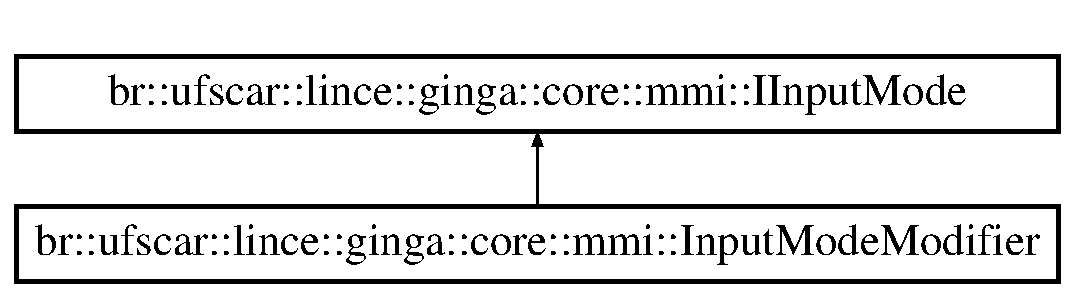
\includegraphics[height=2cm]{classbr_1_1ufscar_1_1lince_1_1ginga_1_1core_1_1mmi_1_1InputModeModifier}
\end{center}
\end{figure}
\subsection*{Métodos Públicos}
\begin{DoxyCompactItemize}
\item 
{\bf InputModeModifier} ()
\item 
{\bf $\sim$InputModeModifier} ()
\item 
virtual IInputEvent $\ast$ {\bf modifierEvent} (IInputEvent $\ast$event)=0
\item 
virtual int {\bf getInputModeType} ()
\end{DoxyCompactItemize}


\subsection{Descrição Detalhada}
Interface que representa um modo de entrada de eventos que realiza modificações nos eventos. 

\subsection{Construtores \& Destrutores}
\index{br::ufscar::lince::ginga::core::mmi::InputModeModifier@{br::ufscar::lince::ginga::core::mmi::InputModeModifier}!InputModeModifier@{InputModeModifier}}
\index{InputModeModifier@{InputModeModifier}!br::ufscar::lince::ginga::core::mmi::InputModeModifier@{br::ufscar::lince::ginga::core::mmi::InputModeModifier}}
\subsubsection[{InputModeModifier}]{\setlength{\rightskip}{0pt plus 5cm}br::ufscar::lince::ginga::core::mmi::InputModeModifier::InputModeModifier ()}\label{classbr_1_1ufscar_1_1lince_1_1ginga_1_1core_1_1mmi_1_1InputModeModifier_ab4218c082d15f30a3e502a13afa74320}
Constrói um modo de entrada modificador. 

Referenciado por $\sim$InputModeModifier().

\index{br::ufscar::lince::ginga::core::mmi::InputModeModifier@{br::ufscar::lince::ginga::core::mmi::InputModeModifier}!$\sim$InputModeModifier@{$\sim$InputModeModifier}}
\index{$\sim$InputModeModifier@{$\sim$InputModeModifier}!br::ufscar::lince::ginga::core::mmi::InputModeModifier@{br::ufscar::lince::ginga::core::mmi::InputModeModifier}}
\subsubsection[{$\sim$InputModeModifier}]{\setlength{\rightskip}{0pt plus 5cm}br::ufscar::lince::ginga::core::mmi::InputModeModifier::$\sim$InputModeModifier ()}\label{classbr_1_1ufscar_1_1lince_1_1ginga_1_1core_1_1mmi_1_1InputModeModifier_a1cf1944c1a2b333fb8f611ae90b3c239}
Destrói um modo de entrada modificador. 

Referências InputModeModifier().



\subsection{Métodos}
\index{br::ufscar::lince::ginga::core::mmi::InputModeModifier@{br::ufscar::lince::ginga::core::mmi::InputModeModifier}!getInputModeType@{getInputModeType}}
\index{getInputModeType@{getInputModeType}!br::ufscar::lince::ginga::core::mmi::InputModeModifier@{br::ufscar::lince::ginga::core::mmi::InputModeModifier}}
\subsubsection[{getInputModeType}]{\setlength{\rightskip}{0pt plus 5cm}int br::ufscar::lince::ginga::core::mmi::InputModeModifier::getInputModeType ()\hspace{0.3cm}{\ttfamily  [virtual]}}\label{classbr_1_1ufscar_1_1lince_1_1ginga_1_1core_1_1mmi_1_1InputModeModifier_a75a4129026ec1170e25defb04d00a1a3}
Retorna a constante inteira que representa o tipo de modo de entrada modificador. \begin{DoxyReturn}{Retorna}
Constante inteira que representa o tipo de modo de entrada modificador. 
\end{DoxyReturn}


Implementa {\bf br::ufscar::lince::ginga::core::mmi::IInputMode} \doxyref{}{pag.}{classbr_1_1ufscar_1_1lince_1_1ginga_1_1core_1_1mmi_1_1IInputMode_a54f7e96cd446cf07e781cd07d55ae99a}.

\index{br::ufscar::lince::ginga::core::mmi::InputModeModifier@{br::ufscar::lince::ginga::core::mmi::InputModeModifier}!modifierEvent@{modifierEvent}}
\index{modifierEvent@{modifierEvent}!br::ufscar::lince::ginga::core::mmi::InputModeModifier@{br::ufscar::lince::ginga::core::mmi::InputModeModifier}}
\subsubsection[{modifierEvent}]{\setlength{\rightskip}{0pt plus 5cm}virtual IInputEvent$\ast$ br::ufscar::lince::ginga::core::mmi::InputModeModifier::modifierEvent (IInputEvent $\ast$ {\em event})\hspace{0.3cm}{\ttfamily  [pure virtual]}}\label{classbr_1_1ufscar_1_1lince_1_1ginga_1_1core_1_1mmi_1_1InputModeModifier_a2f40986cf4645277016d0d923a208b0a}
Módifica o evento de entrada recebido conforme. 
\begin{DoxyParams}{Parâmetros}
\item[{\em event}]evento de entrada a ser modificado. \end{DoxyParams}
\begin{DoxyReturn}{Retorna}
O evento de entrada resultado da modificação. 
\end{DoxyReturn}


A documentação para esta classe foi gerada a partir dos seguintes arquivos:\begin{DoxyCompactItemize}
\item 
include/{\bf InputModeModifier.h}\item 
src/InputModeModifier.cpp\end{DoxyCompactItemize}

\section{Referência da Classe br::ufscar::lince::ginga::core::mmi::InputModeRedirecter}
\label{classbr_1_1ufscar_1_1lince_1_1ginga_1_1core_1_1mmi_1_1InputModeRedirecter}\index{br::ufscar::lince::ginga::core::mmi::InputModeRedirecter@{br::ufscar::lince::ginga::core::mmi::InputModeRedirecter}}


{\ttfamily \#include $<$InputModeRedirecter.h$>$}

Diagrama de Hierarquia para br::ufscar::lince::ginga::core::mmi::InputModeRedirecter:\begin{figure}[H]
\begin{center}
\leavevmode
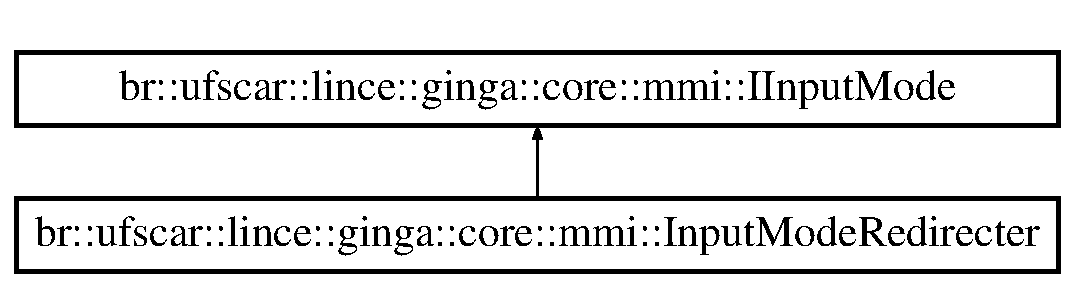
\includegraphics[height=2cm]{classbr_1_1ufscar_1_1lince_1_1ginga_1_1core_1_1mmi_1_1InputModeRedirecter}
\end{center}
\end{figure}
\subsection*{Métodos Públicos}
\begin{DoxyCompactItemize}
\item 
{\bf InputModeRedirecter} ()
\item 
{\bf $\sim$InputModeRedirecter} ()
\item 
virtual int {\bf getInputModeType} ()
\end{DoxyCompactItemize}


\subsection{Descrição Detalhada}
Interface que representa um modo de entrada de eventos que realiza redirecionamento dos eventos. 

\subsection{Construtores \& Destrutores}
\index{br::ufscar::lince::ginga::core::mmi::InputModeRedirecter@{br::ufscar::lince::ginga::core::mmi::InputModeRedirecter}!InputModeRedirecter@{InputModeRedirecter}}
\index{InputModeRedirecter@{InputModeRedirecter}!br::ufscar::lince::ginga::core::mmi::InputModeRedirecter@{br::ufscar::lince::ginga::core::mmi::InputModeRedirecter}}
\subsubsection[{InputModeRedirecter}]{\setlength{\rightskip}{0pt plus 5cm}br::ufscar::lince::ginga::core::mmi::InputModeRedirecter::InputModeRedirecter ()}\label{classbr_1_1ufscar_1_1lince_1_1ginga_1_1core_1_1mmi_1_1InputModeRedirecter_af83a61bea3e91cd6233b862c87819d57}
Constrói um modo de entrada redirecionador. 

Referenciado por $\sim$InputModeRedirecter().

\index{br::ufscar::lince::ginga::core::mmi::InputModeRedirecter@{br::ufscar::lince::ginga::core::mmi::InputModeRedirecter}!$\sim$InputModeRedirecter@{$\sim$InputModeRedirecter}}
\index{$\sim$InputModeRedirecter@{$\sim$InputModeRedirecter}!br::ufscar::lince::ginga::core::mmi::InputModeRedirecter@{br::ufscar::lince::ginga::core::mmi::InputModeRedirecter}}
\subsubsection[{$\sim$InputModeRedirecter}]{\setlength{\rightskip}{0pt plus 5cm}br::ufscar::lince::ginga::core::mmi::InputModeRedirecter::$\sim$InputModeRedirecter ()}\label{classbr_1_1ufscar_1_1lince_1_1ginga_1_1core_1_1mmi_1_1InputModeRedirecter_aad8d8a90629a2e9dd4cc03204de8e60b}
Destrói um modo de entrada redirecionador. 

Referências InputModeRedirecter().



\subsection{Métodos}
\index{br::ufscar::lince::ginga::core::mmi::InputModeRedirecter@{br::ufscar::lince::ginga::core::mmi::InputModeRedirecter}!getInputModeType@{getInputModeType}}
\index{getInputModeType@{getInputModeType}!br::ufscar::lince::ginga::core::mmi::InputModeRedirecter@{br::ufscar::lince::ginga::core::mmi::InputModeRedirecter}}
\subsubsection[{getInputModeType}]{\setlength{\rightskip}{0pt plus 5cm}int br::ufscar::lince::ginga::core::mmi::InputModeRedirecter::getInputModeType ()\hspace{0.3cm}{\ttfamily  [virtual]}}\label{classbr_1_1ufscar_1_1lince_1_1ginga_1_1core_1_1mmi_1_1InputModeRedirecter_a4ede0c5c135504bf4746d1a43b531114}
Retorna a constante inteira que representa o tipo de modo de entrada redirecionador. \begin{DoxyReturn}{Retorna}
Constante inteira que representa o tipo de modo de entrada redirecionador. 
\end{DoxyReturn}


Implementa {\bf br::ufscar::lince::ginga::core::mmi::IInputMode} \doxyref{}{pag.}{classbr_1_1ufscar_1_1lince_1_1ginga_1_1core_1_1mmi_1_1IInputMode_a54f7e96cd446cf07e781cd07d55ae99a}.



A documentação para esta classe foi gerada a partir dos seguintes arquivos:\begin{DoxyCompactItemize}
\item 
include/{\bf InputModeRedirecter.h}\item 
src/InputModeRedirecter.cpp\end{DoxyCompactItemize}

\section{Referência da Estrutura lockedListenerAction}
\label{structlockedListenerAction}\index{lockedListenerAction@{lockedListenerAction}}


{\ttfamily \#include $<$EnhancedInputManager.h$>$}

\subsection*{Atributos Públicos}
\begin{DoxyCompactItemize}
\item 
::br::pucrio::telemidia::ginga::core::system::io::IInputEventListener $\ast$ {\bf l}\label{structlockedListenerAction_a28230643be4f12da017cdde08592e7d5}

\begin{DoxyCompactList}\small\item\em Observador a ser acrescentado ou removido. \item\end{DoxyCompactList}\item 
bool {\bf isAdd}\label{structlockedListenerAction_aa94d3365e82705a04886ca1851fef123}

\begin{DoxyCompactList}\small\item\em Ação a ser realizada. \item\end{DoxyCompactList}\item 
set$<$ int $>$ $\ast$ {\bf events}\label{structlockedListenerAction_a854e24c44ca05d7779d2269cd6a07b7c}

\begin{DoxyCompactList}\small\item\em Conjunto de códigos de tecla nos quais o observador está interessado. \item\end{DoxyCompactList}\end{DoxyCompactItemize}


\subsection{Descrição Detalhada}
Estrutura que representa uma atualização da lista de observadores de eventos. A ação de atualização pode ser de adição ou remoção da lista. 

A documentação para esta estrutura foi gerada a partir do seguinte arquivo:\begin{DoxyCompactItemize}
\item 
include/EnhancedInputManager.h\end{DoxyCompactItemize}

\section{Referência da Estrutura lockedMultimodalListenerAction}
\label{structlockedMultimodalListenerAction}\index{lockedMultimodalListenerAction@{lockedMultimodalListenerAction}}


{\ttfamily \#include $<$EnhancedInputManager.h$>$}

\subsection*{Atributos Públicos}
\begin{DoxyCompactItemize}
\item 
::{\bf br::ufscar::lince::ginga::core::mmi::IMultimodalInputEventListener} $\ast$ {\bf l}\label{structlockedMultimodalListenerAction_ae50b56d7584d1787ceb2bf9cc739821c}

\begin{DoxyCompactList}\small\item\em Observador a ser acrescentado ou removido. \item\end{DoxyCompactList}\item 
bool {\bf isAdd}\label{structlockedMultimodalListenerAction_a5f870f74fde0271b1763a95549dd29eb}

\begin{DoxyCompactList}\small\item\em Ação a ser realizada. \item\end{DoxyCompactList}\end{DoxyCompactItemize}


\subsection{Descrição Detalhada}
Estrutura que representa uma atualização da lista de observadores de eventos multimodais. A ação de atualização pode ser de adição ou remoção da lista. 

A documentação para esta estrutura foi gerada a partir do seguinte arquivo:\begin{DoxyCompactItemize}
\item 
include/EnhancedInputManager.h\end{DoxyCompactItemize}

\section{Referência da Classe br::ufscar::lince::ginga::core::mmi::MultimodalInputEvent}
\label{classbr_1_1ufscar_1_1lince_1_1ginga_1_1core_1_1mmi_1_1MultimodalInputEvent}\index{br::ufscar::lince::ginga::core::mmi::MultimodalInputEvent@{br::ufscar::lince::ginga::core::mmi::MultimodalInputEvent}}


{\ttfamily \#include $<$MultimodalInputEvent.h$>$}

Diagrama de Hierarquia para br::ufscar::lince::ginga::core::mmi::MultimodalInputEvent:\begin{figure}[H]
\begin{center}
\leavevmode
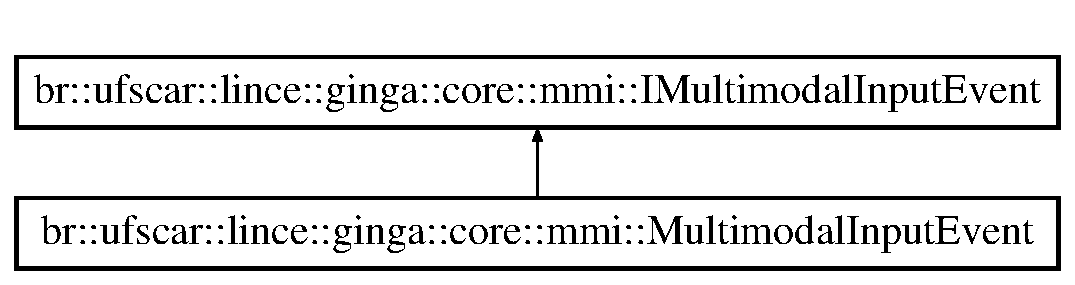
\includegraphics[height=2cm]{classbr_1_1ufscar_1_1lince_1_1ginga_1_1core_1_1mmi_1_1MultimodalInputEvent}
\end{center}
\end{figure}
\subsection*{Métodos Públicos}
\begin{DoxyCompactItemize}
\item 
{\bf MultimodalInputEvent} (string {\bf id})
\item 
{\bf $\sim$MultimodalInputEvent} ()
\item 
virtual string {\bf getId} ()
\item 
virtual void {\bf setId} (string {\bf id})
\item 
void {\bf addValue} (string name, void $\ast$value)
\item 
bool {\bf removeValue} (string name)
\item 
map$<$ string, void $\ast$ $>$ $\ast$ {\bf getMultimodalValuesMap} ()
\item 
void {\bf setMultimodalValuesMap} (map$<$ string, void $\ast$ $>$ $\ast$map)
\item 
virtual vector$<$ string $>$ $\ast$ {\bf getStrings} ()
\item 
virtual void {\bf addString} (string str)
\item 
virtual Ink $\ast$ {\bf getInk} ()
\item 
virtual void {\bf setInk} (Ink $\ast${\bf ink})
\item 
virtual {\bf Acceleration} $\ast$ {\bf getAcceleration} ()
\item 
virtual void {\bf setAcceleration} ({\bf Acceleration} $\ast${\bf accel})
\item 
virtual vector$<$ {\bf File} $\ast$ $>$ $\ast$ {\bf getBinaries} ()
\item 
virtual void {\bf addFile} ({\bf File} $\ast$f)
\end{DoxyCompactItemize}
\subsection*{Atributos Protegidos}
\begin{DoxyCompactItemize}
\item 
string {\bf id}\label{classbr_1_1ufscar_1_1lince_1_1ginga_1_1core_1_1mmi_1_1MultimodalInputEvent_adfe23d6dafe874c4d0f98a4d2cd0e604}

\begin{DoxyCompactList}\small\item\em Variável para definição do id do evento ocorrido. \item\end{DoxyCompactList}\item 
map$<$ string, void $\ast$ $>$ $\ast$ {\bf multimodalValuesMap}\label{classbr_1_1ufscar_1_1lince_1_1ginga_1_1core_1_1mmi_1_1MultimodalInputEvent_a6f781b8c4443cfa943639e74544c50ed}

\begin{DoxyCompactList}\small\item\em Objeto que contém um mapa de chaves e valores. \item\end{DoxyCompactList}\item 
vector$<$ string $>$ $\ast$ {\bf strings}\label{classbr_1_1ufscar_1_1lince_1_1ginga_1_1core_1_1mmi_1_1MultimodalInputEvent_a6dbb0687a3ed96df39d9de44345c79d0}

\begin{DoxyCompactList}\small\item\em Vetor de strings. \item\end{DoxyCompactList}\item 
Ink $\ast$ {\bf ink}\label{classbr_1_1ufscar_1_1lince_1_1ginga_1_1core_1_1mmi_1_1MultimodalInputEvent_aa870673b4559bba8e61955427d2c7fd9}

\begin{DoxyCompactList}\small\item\em Ponteiro par um objeto que guarda os dados de tinta. \item\end{DoxyCompactList}\item 
{\bf Acceleration} $\ast$ {\bf accel}\label{classbr_1_1ufscar_1_1lince_1_1ginga_1_1core_1_1mmi_1_1MultimodalInputEvent_a2b1be3fdbd0e29ea55150df0e37eebdc}

\begin{DoxyCompactList}\small\item\em Ponteiro par um objeto que guarda os dados de acelerômetro. \item\end{DoxyCompactList}\item 
vector$<$ {\bf File} $\ast$ $>$ $\ast$ {\bf binaries}
\begin{DoxyCompactList}\small\item\em Ponteiro par um objeto que guarda os dados de voz. \item\end{DoxyCompactList}\end{DoxyCompactItemize}


\subsection{Descrição Detalhada}
Classe que representa um evento multimodal. 

\subsection{Construtores \& Destrutores}
\index{br::ufscar::lince::ginga::core::mmi::MultimodalInputEvent@{br::ufscar::lince::ginga::core::mmi::MultimodalInputEvent}!MultimodalInputEvent@{MultimodalInputEvent}}
\index{MultimodalInputEvent@{MultimodalInputEvent}!br::ufscar::lince::ginga::core::mmi::MultimodalInputEvent@{br::ufscar::lince::ginga::core::mmi::MultimodalInputEvent}}
\subsubsection[{MultimodalInputEvent}]{\setlength{\rightskip}{0pt plus 5cm}br::ufscar::lince::ginga::core::mmi::MultimodalInputEvent::MultimodalInputEvent (string {\em id})}\label{classbr_1_1ufscar_1_1lince_1_1ginga_1_1core_1_1mmi_1_1MultimodalInputEvent_a279fcc7e312c35c7ed745e5026690e07}
Cria um evento do tipo multimodal apenas definindo seu id 
\begin{DoxyParams}{Parâmetros}
\item[{\em id}]do evento \end{DoxyParams}


Referências binaries, multimodalValuesMap e strings.

\index{br::ufscar::lince::ginga::core::mmi::MultimodalInputEvent@{br::ufscar::lince::ginga::core::mmi::MultimodalInputEvent}!$\sim$MultimodalInputEvent@{$\sim$MultimodalInputEvent}}
\index{$\sim$MultimodalInputEvent@{$\sim$MultimodalInputEvent}!br::ufscar::lince::ginga::core::mmi::MultimodalInputEvent@{br::ufscar::lince::ginga::core::mmi::MultimodalInputEvent}}
\subsubsection[{$\sim$MultimodalInputEvent}]{\setlength{\rightskip}{0pt plus 5cm}br::ufscar::lince::ginga::core::mmi::MultimodalInputEvent::$\sim$MultimodalInputEvent ()}\label{classbr_1_1ufscar_1_1lince_1_1ginga_1_1core_1_1mmi_1_1MultimodalInputEvent_aa0263c1887c689f1cae4bf41b2482ede}
Destrói o objeto do evento multimodal 

Referências binaries, multimodalValuesMap e strings.



\subsection{Métodos}
\index{br::ufscar::lince::ginga::core::mmi::MultimodalInputEvent@{br::ufscar::lince::ginga::core::mmi::MultimodalInputEvent}!addFile@{addFile}}
\index{addFile@{addFile}!br::ufscar::lince::ginga::core::mmi::MultimodalInputEvent@{br::ufscar::lince::ginga::core::mmi::MultimodalInputEvent}}
\subsubsection[{addFile}]{\setlength{\rightskip}{0pt plus 5cm}void br::ufscar::lince::ginga::core::mmi::MultimodalInputEvent::addFile ({\bf File} $\ast$ {\em f})\hspace{0.3cm}{\ttfamily  [virtual]}}\label{classbr_1_1ufscar_1_1lince_1_1ginga_1_1core_1_1mmi_1_1MultimodalInputEvent_ab4d9eb64514f673c9092b4d70fc2bef8}
Adiciona um arquivo ao evento multimodal. 
\begin{DoxyParams}{Parâmetros}
\item[{\em f}]Arquivo a ser adicionad no evento. \end{DoxyParams}


Implementa {\bf br::ufscar::lince::ginga::core::mmi::IMultimodalInputEvent} \doxyref{}{pag.}{classbr_1_1ufscar_1_1lince_1_1ginga_1_1core_1_1mmi_1_1IMultimodalInputEvent_a2202acece2c5b201899ef73a374cb53e}.



Referências binaries.

\index{br::ufscar::lince::ginga::core::mmi::MultimodalInputEvent@{br::ufscar::lince::ginga::core::mmi::MultimodalInputEvent}!addString@{addString}}
\index{addString@{addString}!br::ufscar::lince::ginga::core::mmi::MultimodalInputEvent@{br::ufscar::lince::ginga::core::mmi::MultimodalInputEvent}}
\subsubsection[{addString}]{\setlength{\rightskip}{0pt plus 5cm}void br::ufscar::lince::ginga::core::mmi::MultimodalInputEvent::addString (string {\em str})\hspace{0.3cm}{\ttfamily  [virtual]}}\label{classbr_1_1ufscar_1_1lince_1_1ginga_1_1core_1_1mmi_1_1MultimodalInputEvent_af375eab32140b0faa2f860feee4c5870}
Adiciona uma string ao evento multimodal. 
\begin{DoxyParams}{Parâmetros}
\item[{\em str}]String a ser adicionada no evento. \end{DoxyParams}


Implementa {\bf br::ufscar::lince::ginga::core::mmi::IMultimodalInputEvent} \doxyref{}{pag.}{classbr_1_1ufscar_1_1lince_1_1ginga_1_1core_1_1mmi_1_1IMultimodalInputEvent_a17f4a388d7854789b10d68615b098d56}.



Referências strings.

\index{br::ufscar::lince::ginga::core::mmi::MultimodalInputEvent@{br::ufscar::lince::ginga::core::mmi::MultimodalInputEvent}!addValue@{addValue}}
\index{addValue@{addValue}!br::ufscar::lince::ginga::core::mmi::MultimodalInputEvent@{br::ufscar::lince::ginga::core::mmi::MultimodalInputEvent}}
\subsubsection[{addValue}]{\setlength{\rightskip}{0pt plus 5cm}void br::ufscar::lince::ginga::core::mmi::MultimodalInputEvent::addValue (string {\em name}, \/  void $\ast$ {\em value})\hspace{0.3cm}{\ttfamily  [virtual]}}\label{classbr_1_1ufscar_1_1lince_1_1ginga_1_1core_1_1mmi_1_1MultimodalInputEvent_a35451b8fa11bb048860f738268bfdf1c}
Adiciona novos valores ao evento multimodal 
\begin{DoxyParams}{Parâmetros}
\item[{\em name}]Nome do valor \item[{\em value}]O valor \end{DoxyParams}


Implementa {\bf br::ufscar::lince::ginga::core::mmi::IMultimodalInputEvent} \doxyref{}{pag.}{classbr_1_1ufscar_1_1lince_1_1ginga_1_1core_1_1mmi_1_1IMultimodalInputEvent_ad10863e1dbfe978e89729ad629edb815}.



Referências multimodalValuesMap.

\index{br::ufscar::lince::ginga::core::mmi::MultimodalInputEvent@{br::ufscar::lince::ginga::core::mmi::MultimodalInputEvent}!getAcceleration@{getAcceleration}}
\index{getAcceleration@{getAcceleration}!br::ufscar::lince::ginga::core::mmi::MultimodalInputEvent@{br::ufscar::lince::ginga::core::mmi::MultimodalInputEvent}}
\subsubsection[{getAcceleration}]{\setlength{\rightskip}{0pt plus 5cm}{\bf Acceleration} $\ast$ br::ufscar::lince::ginga::core::mmi::MultimodalInputEvent::getAcceleration ()\hspace{0.3cm}{\ttfamily  [virtual]}}\label{classbr_1_1ufscar_1_1lince_1_1ginga_1_1core_1_1mmi_1_1MultimodalInputEvent_ada47dfbfd8048f03f96c336ef4f9ec75}
Acessa o objeto acceleration do evento multimodal. \begin{DoxyReturn}{Retorna}
objeto \doxyref{Acceleration}{pag.}{classbr_1_1ufscar_1_1lince_1_1ginga_1_1core_1_1mmi_1_1Acceleration} com os dados de aceleração do evento. 
\end{DoxyReturn}


Implementa {\bf br::ufscar::lince::ginga::core::mmi::IMultimodalInputEvent} \doxyref{}{pag.}{classbr_1_1ufscar_1_1lince_1_1ginga_1_1core_1_1mmi_1_1IMultimodalInputEvent_a9ed35bcbcbb3cbb20b050d5665d9ff35}.



Referências accel.

\index{br::ufscar::lince::ginga::core::mmi::MultimodalInputEvent@{br::ufscar::lince::ginga::core::mmi::MultimodalInputEvent}!getBinaries@{getBinaries}}
\index{getBinaries@{getBinaries}!br::ufscar::lince::ginga::core::mmi::MultimodalInputEvent@{br::ufscar::lince::ginga::core::mmi::MultimodalInputEvent}}
\subsubsection[{getBinaries}]{\setlength{\rightskip}{0pt plus 5cm}vector$<$ {\bf File} $\ast$ $>$ $\ast$ br::ufscar::lince::ginga::core::mmi::MultimodalInputEvent::getBinaries ()\hspace{0.3cm}{\ttfamily  [virtual]}}\label{classbr_1_1ufscar_1_1lince_1_1ginga_1_1core_1_1mmi_1_1MultimodalInputEvent_a4abcfcedec49098c0279db3097433f29}
Acessa os arquivos do evento multimodal. \begin{DoxyReturn}{Retorna}
vetor de arquivos. 
\end{DoxyReturn}


Implementa {\bf br::ufscar::lince::ginga::core::mmi::IMultimodalInputEvent} \doxyref{}{pag.}{classbr_1_1ufscar_1_1lince_1_1ginga_1_1core_1_1mmi_1_1IMultimodalInputEvent_a3616b43630e332773c482d6406c00a2f}.



Referências binaries.

\index{br::ufscar::lince::ginga::core::mmi::MultimodalInputEvent@{br::ufscar::lince::ginga::core::mmi::MultimodalInputEvent}!getId@{getId}}
\index{getId@{getId}!br::ufscar::lince::ginga::core::mmi::MultimodalInputEvent@{br::ufscar::lince::ginga::core::mmi::MultimodalInputEvent}}
\subsubsection[{getId}]{\setlength{\rightskip}{0pt plus 5cm}string br::ufscar::lince::ginga::core::mmi::MultimodalInputEvent::getId ()\hspace{0.3cm}{\ttfamily  [virtual]}}\label{classbr_1_1ufscar_1_1lince_1_1ginga_1_1core_1_1mmi_1_1MultimodalInputEvent_a1a6648f772f8ae29244dbfccd61c1e61}
Acessa o id do evento multimodal. \begin{DoxyReturn}{Retorna}
id do evento. 
\end{DoxyReturn}


Implementa {\bf br::ufscar::lince::ginga::core::mmi::IMultimodalInputEvent} \doxyref{}{pag.}{classbr_1_1ufscar_1_1lince_1_1ginga_1_1core_1_1mmi_1_1IMultimodalInputEvent_a61a42387f2e29c30639905079695d8f8}.



Referências id.

\index{br::ufscar::lince::ginga::core::mmi::MultimodalInputEvent@{br::ufscar::lince::ginga::core::mmi::MultimodalInputEvent}!getInk@{getInk}}
\index{getInk@{getInk}!br::ufscar::lince::ginga::core::mmi::MultimodalInputEvent@{br::ufscar::lince::ginga::core::mmi::MultimodalInputEvent}}
\subsubsection[{getInk}]{\setlength{\rightskip}{0pt plus 5cm}Ink $\ast$ br::ufscar::lince::ginga::core::mmi::MultimodalInputEvent::getInk ()\hspace{0.3cm}{\ttfamily  [virtual]}}\label{classbr_1_1ufscar_1_1lince_1_1ginga_1_1core_1_1mmi_1_1MultimodalInputEvent_ac1dcabf82763009c60dfc3c63c43ec1a}
Acessa o objeto ink do evento multimodal. \begin{DoxyReturn}{Retorna}
ink objeto com os dados de tinta do evento. 
\end{DoxyReturn}


Implementa {\bf br::ufscar::lince::ginga::core::mmi::IMultimodalInputEvent} \doxyref{}{pag.}{classbr_1_1ufscar_1_1lince_1_1ginga_1_1core_1_1mmi_1_1IMultimodalInputEvent_a23a24cc399ceb022a43a60c46ae6a6d9}.



Referências ink.

\index{br::ufscar::lince::ginga::core::mmi::MultimodalInputEvent@{br::ufscar::lince::ginga::core::mmi::MultimodalInputEvent}!getMultimodalValuesMap@{getMultimodalValuesMap}}
\index{getMultimodalValuesMap@{getMultimodalValuesMap}!br::ufscar::lince::ginga::core::mmi::MultimodalInputEvent@{br::ufscar::lince::ginga::core::mmi::MultimodalInputEvent}}
\subsubsection[{getMultimodalValuesMap}]{\setlength{\rightskip}{0pt plus 5cm}map$<$ string, void $\ast$ $>$ $\ast$ br::ufscar::lince::ginga::core::mmi::MultimodalInputEvent::getMultimodalValuesMap ()\hspace{0.3cm}{\ttfamily  [virtual]}}\label{classbr_1_1ufscar_1_1lince_1_1ginga_1_1core_1_1mmi_1_1MultimodalInputEvent_abafe975af04a1680cc8184fcba8de6a4}
Acessa os valores contidos no evento multimodal \begin{DoxyReturn}{Retorna}
mapa com todos os valores contidos no evento multimodal 
\end{DoxyReturn}


Implementa {\bf br::ufscar::lince::ginga::core::mmi::IMultimodalInputEvent} \doxyref{}{pag.}{classbr_1_1ufscar_1_1lince_1_1ginga_1_1core_1_1mmi_1_1IMultimodalInputEvent_a2063d0a8661ed4e178bab240c91cc014}.



Referências multimodalValuesMap.

\index{br::ufscar::lince::ginga::core::mmi::MultimodalInputEvent@{br::ufscar::lince::ginga::core::mmi::MultimodalInputEvent}!getStrings@{getStrings}}
\index{getStrings@{getStrings}!br::ufscar::lince::ginga::core::mmi::MultimodalInputEvent@{br::ufscar::lince::ginga::core::mmi::MultimodalInputEvent}}
\subsubsection[{getStrings}]{\setlength{\rightskip}{0pt plus 5cm}vector$<$ string $>$ $\ast$ br::ufscar::lince::ginga::core::mmi::MultimodalInputEvent::getStrings ()\hspace{0.3cm}{\ttfamily  [virtual]}}\label{classbr_1_1ufscar_1_1lince_1_1ginga_1_1core_1_1mmi_1_1MultimodalInputEvent_ae9a66008d133d84eb977dad43b379ae5}
Acessa as strings do evento multimodal. \begin{DoxyReturn}{Retorna}
vetor de strings. 
\end{DoxyReturn}


Implementa {\bf br::ufscar::lince::ginga::core::mmi::IMultimodalInputEvent} \doxyref{}{pag.}{classbr_1_1ufscar_1_1lince_1_1ginga_1_1core_1_1mmi_1_1IMultimodalInputEvent_a41a14202b17c64e7d0216d47bfeebfd9}.



Referências strings.

\index{br::ufscar::lince::ginga::core::mmi::MultimodalInputEvent@{br::ufscar::lince::ginga::core::mmi::MultimodalInputEvent}!removeValue@{removeValue}}
\index{removeValue@{removeValue}!br::ufscar::lince::ginga::core::mmi::MultimodalInputEvent@{br::ufscar::lince::ginga::core::mmi::MultimodalInputEvent}}
\subsubsection[{removeValue}]{\setlength{\rightskip}{0pt plus 5cm}bool br::ufscar::lince::ginga::core::mmi::MultimodalInputEvent::removeValue (string {\em name})\hspace{0.3cm}{\ttfamily  [virtual]}}\label{classbr_1_1ufscar_1_1lince_1_1ginga_1_1core_1_1mmi_1_1MultimodalInputEvent_acb330a03e341bbf051aaf2a44c640b86}
Remove valores do evento multimodal 
\begin{DoxyParams}{Parâmetros}
\item[{\em name}]Nome do valor \end{DoxyParams}
\begin{DoxyReturn}{Retorna}
true caso o valor tenha sido removido 

false caso o valor não tenha sido removido 
\end{DoxyReturn}


Implementa {\bf br::ufscar::lince::ginga::core::mmi::IMultimodalInputEvent} \doxyref{}{pag.}{classbr_1_1ufscar_1_1lince_1_1ginga_1_1core_1_1mmi_1_1IMultimodalInputEvent_adfcffaf158db42a0d0fb6e522faad91f}.

\index{br::ufscar::lince::ginga::core::mmi::MultimodalInputEvent@{br::ufscar::lince::ginga::core::mmi::MultimodalInputEvent}!setAcceleration@{setAcceleration}}
\index{setAcceleration@{setAcceleration}!br::ufscar::lince::ginga::core::mmi::MultimodalInputEvent@{br::ufscar::lince::ginga::core::mmi::MultimodalInputEvent}}
\subsubsection[{setAcceleration}]{\setlength{\rightskip}{0pt plus 5cm}void br::ufscar::lince::ginga::core::mmi::MultimodalInputEvent::setAcceleration ({\bf Acceleration} $\ast$ {\em accel})\hspace{0.3cm}{\ttfamily  [virtual]}}\label{classbr_1_1ufscar_1_1lince_1_1ginga_1_1core_1_1mmi_1_1MultimodalInputEvent_a5f9638fa3fc331ab11e1aca30bc33035}
Define o objeto acceleration do evento multimodal. 
\begin{DoxyParams}{Parâmetros}
\item[{\em accel}]objeto com os dados de aceleração do evento. \end{DoxyParams}


Implementa {\bf br::ufscar::lince::ginga::core::mmi::IMultimodalInputEvent} \doxyref{}{pag.}{classbr_1_1ufscar_1_1lince_1_1ginga_1_1core_1_1mmi_1_1IMultimodalInputEvent_a9ba0b45f1919bbfbe08bc0267a7452eb}.

\index{br::ufscar::lince::ginga::core::mmi::MultimodalInputEvent@{br::ufscar::lince::ginga::core::mmi::MultimodalInputEvent}!setId@{setId}}
\index{setId@{setId}!br::ufscar::lince::ginga::core::mmi::MultimodalInputEvent@{br::ufscar::lince::ginga::core::mmi::MultimodalInputEvent}}
\subsubsection[{setId}]{\setlength{\rightskip}{0pt plus 5cm}void br::ufscar::lince::ginga::core::mmi::MultimodalInputEvent::setId (string {\em id})\hspace{0.3cm}{\ttfamily  [virtual]}}\label{classbr_1_1ufscar_1_1lince_1_1ginga_1_1core_1_1mmi_1_1MultimodalInputEvent_a5de98758c900a1523f3b52310c59b056}
Define o id do evento multimodal. 
\begin{DoxyParams}{Parâmetros}
\item[{\em id}]do evento. \end{DoxyParams}


Implementa {\bf br::ufscar::lince::ginga::core::mmi::IMultimodalInputEvent} \doxyref{}{pag.}{classbr_1_1ufscar_1_1lince_1_1ginga_1_1core_1_1mmi_1_1IMultimodalInputEvent_aaaa1d0a0d5d196e2b3e43573404f2cca}.

\index{br::ufscar::lince::ginga::core::mmi::MultimodalInputEvent@{br::ufscar::lince::ginga::core::mmi::MultimodalInputEvent}!setInk@{setInk}}
\index{setInk@{setInk}!br::ufscar::lince::ginga::core::mmi::MultimodalInputEvent@{br::ufscar::lince::ginga::core::mmi::MultimodalInputEvent}}
\subsubsection[{setInk}]{\setlength{\rightskip}{0pt plus 5cm}void br::ufscar::lince::ginga::core::mmi::MultimodalInputEvent::setInk (Ink $\ast$ {\em ink})\hspace{0.3cm}{\ttfamily  [virtual]}}\label{classbr_1_1ufscar_1_1lince_1_1ginga_1_1core_1_1mmi_1_1MultimodalInputEvent_aa5b3575f54367657785e5dbae5139646}
Define o objeto ink do evento multimodal. 
\begin{DoxyParams}{Parâmetros}
\item[{\em ink}]objeto com os dados de tinta do evento. \end{DoxyParams}


Implementa {\bf br::ufscar::lince::ginga::core::mmi::IMultimodalInputEvent} \doxyref{}{pag.}{classbr_1_1ufscar_1_1lince_1_1ginga_1_1core_1_1mmi_1_1IMultimodalInputEvent_a2d7da14262a0127f188f69a72ec4a5de}.

\index{br::ufscar::lince::ginga::core::mmi::MultimodalInputEvent@{br::ufscar::lince::ginga::core::mmi::MultimodalInputEvent}!setMultimodalValuesMap@{setMultimodalValuesMap}}
\index{setMultimodalValuesMap@{setMultimodalValuesMap}!br::ufscar::lince::ginga::core::mmi::MultimodalInputEvent@{br::ufscar::lince::ginga::core::mmi::MultimodalInputEvent}}
\subsubsection[{setMultimodalValuesMap}]{\setlength{\rightskip}{0pt plus 5cm}void br::ufscar::lince::ginga::core::mmi::MultimodalInputEvent::setMultimodalValuesMap (map$<$ string, void $\ast$ $>$ $\ast$ {\em map})\hspace{0.3cm}{\ttfamily  [virtual]}}\label{classbr_1_1ufscar_1_1lince_1_1ginga_1_1core_1_1mmi_1_1MultimodalInputEvent_a1d8c120f0c93b3ada06e6c3c165b0aea}
Define um mapa com valores ao evento multimodal 
\begin{DoxyParams}{Parâmetros}
\item[{\em map}]Mapa com todos os valores a serem inseridos no evento multimodal \end{DoxyParams}


Implementa {\bf br::ufscar::lince::ginga::core::mmi::IMultimodalInputEvent} \doxyref{}{pag.}{classbr_1_1ufscar_1_1lince_1_1ginga_1_1core_1_1mmi_1_1IMultimodalInputEvent_ac9d69cb5bae636bf164d620dfb8c5d75}.



Referências multimodalValuesMap.



\subsection{Atributos}
\index{br::ufscar::lince::ginga::core::mmi::MultimodalInputEvent@{br::ufscar::lince::ginga::core::mmi::MultimodalInputEvent}!binaries@{binaries}}
\index{binaries@{binaries}!br::ufscar::lince::ginga::core::mmi::MultimodalInputEvent@{br::ufscar::lince::ginga::core::mmi::MultimodalInputEvent}}
\subsubsection[{binaries}]{\setlength{\rightskip}{0pt plus 5cm}vector$<${\bf File}$\ast$$>$$\ast$ {\bf br::ufscar::lince::ginga::core::mmi::MultimodalInputEvent::binaries}\hspace{0.3cm}{\ttfamily  [protected]}}\label{classbr_1_1ufscar_1_1lince_1_1ginga_1_1core_1_1mmi_1_1MultimodalInputEvent_a7ebd98f88b4e48ad20d11715ebeda49a}


Ponteiro par um objeto que guarda os dados de voz. 

Vetor de arquivos 

Referenciado por addFile(), getBinaries(), MultimodalInputEvent() e $\sim$MultimodalInputEvent().



A documentação para esta classe foi gerada a partir dos seguintes arquivos:\begin{DoxyCompactItemize}
\item 
include/{\bf MultimodalInputEvent.h}\item 
src/{\bf MultimodalInputEvent.cpp}\end{DoxyCompactItemize}

\section{Referência da Estrutura br::ufscar::lince::ginga::core::mmi::inkmllib::structBoundingBox}
\label{structbr_1_1ufscar_1_1lince_1_1ginga_1_1core_1_1mmi_1_1inkmllib_1_1structBoundingBox}\index{br::ufscar::lince::ginga::core::mmi::inkmllib::structBoundingBox@{br::ufscar::lince::ginga::core::mmi::inkmllib::structBoundingBox}}


{\ttfamily \#include $<$Utility.h$>$}

\subsection*{Atributos Públicos}
\begin{DoxyCompactItemize}
\item 
long {\bf minX}\label{structbr_1_1ufscar_1_1lince_1_1ginga_1_1core_1_1mmi_1_1inkmllib_1_1structBoundingBox_a909b122c96d0e5584c519a0944b5fc6a}

\begin{DoxyCompactList}\small\item\em Limite inferior horizontal. \item\end{DoxyCompactList}\item 
long {\bf minY}\label{structbr_1_1ufscar_1_1lince_1_1ginga_1_1core_1_1mmi_1_1inkmllib_1_1structBoundingBox_a776577ef30a54223fd275f07f0bff36a}

\begin{DoxyCompactList}\small\item\em Limite superior vertical. \item\end{DoxyCompactList}\item 
long {\bf maxX}\label{structbr_1_1ufscar_1_1lince_1_1ginga_1_1core_1_1mmi_1_1inkmllib_1_1structBoundingBox_af5f666e90db4a721765db9884da8affe}

\begin{DoxyCompactList}\small\item\em Limite superior horizontal. \item\end{DoxyCompactList}\item 
long {\bf maxY}\label{structbr_1_1ufscar_1_1lince_1_1ginga_1_1core_1_1mmi_1_1inkmllib_1_1structBoundingBox_a8f05573019dd330229cebf9af20eb067}

\begin{DoxyCompactList}\small\item\em Limite inferior vertical. \item\end{DoxyCompactList}\end{DoxyCompactItemize}


\subsection{Descrição Detalhada}
Desc -\/ structure to define the BoundingBox of the trace data and hence helps in normalizing trace co-\/ordinate data to fit in the rendering area co-\/ordinate. 

A documentação para esta estrutura foi gerada a partir do seguinte arquivo:\begin{DoxyCompactItemize}
\item 
include/Utility.h\end{DoxyCompactItemize}

\section{Referência da Classe br::ufscar::lince::ginga::core::mmi::inkmllib::Trace}
\label{classbr_1_1ufscar_1_1lince_1_1ginga_1_1core_1_1mmi_1_1inkmllib_1_1Trace}\index{br::ufscar::lince::ginga::core::mmi::inkmllib::Trace@{br::ufscar::lince::ginga::core::mmi::inkmllib::Trace}}


{\ttfamily \#include $<$Trace.h$>$}

\subsection*{Métodos Públicos}
\begin{DoxyCompactItemize}
\item 
{\bf Trace} ()
\item 
void {\bf setTraceFormatRef} ({\bf TraceFormat} $\ast${\bf traceFormatRef})
\item 
void {\bf parseTraceData} (char $\ast$data, {\bf BoundingBox} $\ast$boundingBox)
\end{DoxyCompactItemize}
\subsection*{Atributos Públicos}
\begin{DoxyCompactItemize}
\item 
{\bf TraceFormat} $\ast$ {\bf traceFormatRef}
\item 
vector$<$ long $>$ $\ast$ {\bf vectX}
\item 
vector$<$ long $>$ $\ast$ {\bf vectY}
\item 
vector$<$ int $>$ $\ast$ {\bf vectF}
\end{DoxyCompactItemize}


\subsection{Descrição Detalhada}
Classe que representa um trace de um InkML. Mais informações em {\tt http://sourceforge.net/apps/trac/inkmltk/wiki/InkMLLib} 

\subsection{Construtores \& Destrutores}
\index{br::ufscar::lince::ginga::core::mmi::inkmllib::Trace@{br::ufscar::lince::ginga::core::mmi::inkmllib::Trace}!Trace@{Trace}}
\index{Trace@{Trace}!br::ufscar::lince::ginga::core::mmi::inkmllib::Trace@{br::ufscar::lince::ginga::core::mmi::inkmllib::Trace}}
\subsubsection[{Trace}]{\setlength{\rightskip}{0pt plus 5cm}br::ufscar::lince::ginga::core::mmi::inkmllib::Trace::Trace ()}\label{classbr_1_1ufscar_1_1lince_1_1ginga_1_1core_1_1mmi_1_1inkmllib_1_1Trace_abc01a59768ea5f24bb7eafb779b56139}
Desc -\/ constructor.

Desc -\/ constructor 

Referências traceFormatRef, vectF, vectX e vectY.



\subsection{Métodos}
\index{br::ufscar::lince::ginga::core::mmi::inkmllib::Trace@{br::ufscar::lince::ginga::core::mmi::inkmllib::Trace}!parseTraceData@{parseTraceData}}
\index{parseTraceData@{parseTraceData}!br::ufscar::lince::ginga::core::mmi::inkmllib::Trace@{br::ufscar::lince::ginga::core::mmi::inkmllib::Trace}}
\subsubsection[{parseTraceData}]{\setlength{\rightskip}{0pt plus 5cm}void br::ufscar::lince::ginga::core::mmi::inkmllib::Trace::parseTraceData (char $\ast$ {\em data}, \/  {\bf BoundingBox} $\ast$ {\em boundingBox})}\label{classbr_1_1ufscar_1_1lince_1_1ginga_1_1core_1_1mmi_1_1inkmllib_1_1Trace_adf17d60b513b1aef583234205ecc8ffd}
Desc -\/ function to parse traceData. It uses the setDataCoordinate method to process and store co-\/ordinate values. 

Referências br::ufscar::lince::ginga::core::mmi::inkmllib::TraceFormat::getChannelAtIndex() e traceFormatRef.



Referenciado por br::ufscar::lince::ginga::core::mmi::inkmllib::InkMLParser::insertTrace().

\index{br::ufscar::lince::ginga::core::mmi::inkmllib::Trace@{br::ufscar::lince::ginga::core::mmi::inkmllib::Trace}!setTraceFormatRef@{setTraceFormatRef}}
\index{setTraceFormatRef@{setTraceFormatRef}!br::ufscar::lince::ginga::core::mmi::inkmllib::Trace@{br::ufscar::lince::ginga::core::mmi::inkmllib::Trace}}
\subsubsection[{setTraceFormatRef}]{\setlength{\rightskip}{0pt plus 5cm}void br::ufscar::lince::ginga::core::mmi::inkmllib::Trace::setTraceFormatRef ({\bf TraceFormat} $\ast$ {\em traceFormatRef})\hspace{0.3cm}{\ttfamily  [inline]}}\label{classbr_1_1ufscar_1_1lince_1_1ginga_1_1core_1_1mmi_1_1inkmllib_1_1Trace_a86a974cd4bdf8df5c2c764cba055d3cf}
Desc -\/ assign traceFormat of this trace. 

Referenciado por br::ufscar::lince::ginga::core::mmi::inkmllib::InkMLParser::insertTrace().



\subsection{Atributos}
\index{br::ufscar::lince::ginga::core::mmi::inkmllib::Trace@{br::ufscar::lince::ginga::core::mmi::inkmllib::Trace}!traceFormatRef@{traceFormatRef}}
\index{traceFormatRef@{traceFormatRef}!br::ufscar::lince::ginga::core::mmi::inkmllib::Trace@{br::ufscar::lince::ginga::core::mmi::inkmllib::Trace}}
\subsubsection[{traceFormatRef}]{\setlength{\rightskip}{0pt plus 5cm}{\bf TraceFormat}$\ast$ {\bf br::ufscar::lince::ginga::core::mmi::inkmllib::Trace::traceFormatRef}}\label{classbr_1_1ufscar_1_1lince_1_1ginga_1_1core_1_1mmi_1_1inkmllib_1_1Trace_a788feb85d559a31b53354a5b19ff09c6}
Desc -\/ Reference to the associated \doxyref{TraceFormat}{pag.}{classbr_1_1ufscar_1_1lince_1_1ginga_1_1core_1_1mmi_1_1inkmllib_1_1TraceFormat}. 

Referenciado por parseTraceData() e Trace().

\index{br::ufscar::lince::ginga::core::mmi::inkmllib::Trace@{br::ufscar::lince::ginga::core::mmi::inkmllib::Trace}!vectF@{vectF}}
\index{vectF@{vectF}!br::ufscar::lince::ginga::core::mmi::inkmllib::Trace@{br::ufscar::lince::ginga::core::mmi::inkmllib::Trace}}
\subsubsection[{vectF}]{\setlength{\rightskip}{0pt plus 5cm}vector$<$int$>$$\ast$ {\bf br::ufscar::lince::ginga::core::mmi::inkmllib::Trace::vectF}}\label{classbr_1_1ufscar_1_1lince_1_1ginga_1_1core_1_1mmi_1_1inkmllib_1_1Trace_a717bfb26b8cc5d13cde200b1eee46dba}
Desc -\/ To hold channel F data (i.e. Pressure/Force co-\/ordinate data). 

Referenciado por Trace().

\index{br::ufscar::lince::ginga::core::mmi::inkmllib::Trace@{br::ufscar::lince::ginga::core::mmi::inkmllib::Trace}!vectX@{vectX}}
\index{vectX@{vectX}!br::ufscar::lince::ginga::core::mmi::inkmllib::Trace@{br::ufscar::lince::ginga::core::mmi::inkmllib::Trace}}
\subsubsection[{vectX}]{\setlength{\rightskip}{0pt plus 5cm}vector$<$long$>$$\ast$ {\bf br::ufscar::lince::ginga::core::mmi::inkmllib::Trace::vectX}}\label{classbr_1_1ufscar_1_1lince_1_1ginga_1_1core_1_1mmi_1_1inkmllib_1_1Trace_a86f550f28331c427cb0214826832f100}
Desc -\/ To hold channel X data (i.e. X co-\/ordinate data). 

Referenciado por br::ufscar::lince::ginga::core::mmi::inkmllib::Ink::normalizeTracePoint() e Trace().

\index{br::ufscar::lince::ginga::core::mmi::inkmllib::Trace@{br::ufscar::lince::ginga::core::mmi::inkmllib::Trace}!vectY@{vectY}}
\index{vectY@{vectY}!br::ufscar::lince::ginga::core::mmi::inkmllib::Trace@{br::ufscar::lince::ginga::core::mmi::inkmllib::Trace}}
\subsubsection[{vectY}]{\setlength{\rightskip}{0pt plus 5cm}vector$<$long$>$$\ast$ {\bf br::ufscar::lince::ginga::core::mmi::inkmllib::Trace::vectY}}\label{classbr_1_1ufscar_1_1lince_1_1ginga_1_1core_1_1mmi_1_1inkmllib_1_1Trace_a8d478fda07ddaa3c8297257fb6f0ea79}
Desc -\/ To hold channel Y data (i.e. Y co-\/ordinate data). 

Referenciado por br::ufscar::lince::ginga::core::mmi::inkmllib::Ink::normalizeTracePoint() e Trace().



A documentação para esta classe foi gerada a partir dos seguintes arquivos:\begin{DoxyCompactItemize}
\item 
include/Trace.h\item 
src/Trace.cpp\end{DoxyCompactItemize}

\section{Referência da Classe br::ufscar::lince::ginga::core::mmi::inkmllib::TraceFormat}
\label{classbr_1_1ufscar_1_1lince_1_1ginga_1_1core_1_1mmi_1_1inkmllib_1_1TraceFormat}\index{br::ufscar::lince::ginga::core::mmi::inkmllib::TraceFormat@{br::ufscar::lince::ginga::core::mmi::inkmllib::TraceFormat}}


{\ttfamily \#include $<$TraceFormat.h$>$}

\subsection*{Métodos Públicos}
\begin{DoxyCompactItemize}
\item 
{\bf TraceFormat} ()
\item 
{\bf TraceFormat} (char $\ast${\bf id})
\item 
void {\bf addChannelOrder} (CHANNEL c)
\item 
char $\ast$ {\bf getID} ()
\item 
CHANNEL {\bf getChannelAtIndex} (int index)
\item 
void {\bf addChannelOrder} (char $\ast$c)
\end{DoxyCompactItemize}
\subsection*{Atributos Públicos}
\begin{DoxyCompactItemize}
\item 
char $\ast$ {\bf id}\label{classbr_1_1ufscar_1_1lince_1_1ginga_1_1core_1_1mmi_1_1inkmllib_1_1TraceFormat_abea6b0aaf271558a97e152cfb91444da}

\begin{DoxyCompactList}\small\item\em Id do traceFormat. \item\end{DoxyCompactList}\item 
bool {\bf channelFPresent}
\item 
vector$<$ {\bf Channel} $>$ $\ast$ {\bf vectChannel}\label{classbr_1_1ufscar_1_1lince_1_1ginga_1_1core_1_1mmi_1_1inkmllib_1_1TraceFormat_a2b46b43d288be14cd49f84b680ca49ce}

\begin{DoxyCompactList}\small\item\em Lista de channels. \item\end{DoxyCompactList}\item 
vector$<$ CHANNEL $>$ $\ast$ {\bf vectChannelOrder}\label{classbr_1_1ufscar_1_1lince_1_1ginga_1_1core_1_1mmi_1_1inkmllib_1_1TraceFormat_a59710257ae03cbd54cf3d97f46b440f8}

\begin{DoxyCompactList}\small\item\em Lista de channels. \item\end{DoxyCompactList}\end{DoxyCompactItemize}


\subsection{Descrição Detalhada}
Classe que representa o formato de um trace de um InkML. Mais informações em {\tt http://sourceforge.net/apps/trac/inkmltk/wiki/InkMLLib} 

\subsection{Construtores \& Destrutores}
\index{br::ufscar::lince::ginga::core::mmi::inkmllib::TraceFormat@{br::ufscar::lince::ginga::core::mmi::inkmllib::TraceFormat}!TraceFormat@{TraceFormat}}
\index{TraceFormat@{TraceFormat}!br::ufscar::lince::ginga::core::mmi::inkmllib::TraceFormat@{br::ufscar::lince::ginga::core::mmi::inkmllib::TraceFormat}}
\subsubsection[{TraceFormat}]{\setlength{\rightskip}{0pt plus 5cm}br::ufscar::lince::ginga::core::mmi::inkmllib::TraceFormat::TraceFormat ()}\label{classbr_1_1ufscar_1_1lince_1_1ginga_1_1core_1_1mmi_1_1inkmllib_1_1TraceFormat_a0796113a07aa206d2d1c840fa244058b}
Desc -\/ Constructor 

Referências channelFPresent, vectChannel e vectChannelOrder.

\index{br::ufscar::lince::ginga::core::mmi::inkmllib::TraceFormat@{br::ufscar::lince::ginga::core::mmi::inkmllib::TraceFormat}!TraceFormat@{TraceFormat}}
\index{TraceFormat@{TraceFormat}!br::ufscar::lince::ginga::core::mmi::inkmllib::TraceFormat@{br::ufscar::lince::ginga::core::mmi::inkmllib::TraceFormat}}
\subsubsection[{TraceFormat}]{\setlength{\rightskip}{0pt plus 5cm}br::ufscar::lince::ginga::core::mmi::inkmllib::TraceFormat::TraceFormat (char $\ast$ {\em id})}\label{classbr_1_1ufscar_1_1lince_1_1ginga_1_1core_1_1mmi_1_1inkmllib_1_1TraceFormat_aa92ce1c7c122ffff651e2d70cf2a448d}
Construtor 
\begin{DoxyParams}{Parâmetros}
\item[{\em id}]do traceFormat. \end{DoxyParams}


Referências channelFPresent, vectChannel e vectChannelOrder.



\subsection{Métodos}
\index{br::ufscar::lince::ginga::core::mmi::inkmllib::TraceFormat@{br::ufscar::lince::ginga::core::mmi::inkmllib::TraceFormat}!addChannelOrder@{addChannelOrder}}
\index{addChannelOrder@{addChannelOrder}!br::ufscar::lince::ginga::core::mmi::inkmllib::TraceFormat@{br::ufscar::lince::ginga::core::mmi::inkmllib::TraceFormat}}
\subsubsection[{addChannelOrder}]{\setlength{\rightskip}{0pt plus 5cm}void br::ufscar::lince::ginga::core::mmi::inkmllib::TraceFormat::addChannelOrder (char $\ast$ {\em c})}\label{classbr_1_1ufscar_1_1lince_1_1ginga_1_1core_1_1mmi_1_1inkmllib_1_1TraceFormat_ac238cb7dd873135c37a48791928eac5d}
Adiciona um channel. 
\begin{DoxyParams}{Parâmetros}
\item[{\em c}]\doxyref{Channel}{pag.}{classbr_1_1ufscar_1_1lince_1_1ginga_1_1core_1_1mmi_1_1inkmllib_1_1Channel} a ser adicionado. \end{DoxyParams}


Referências br::ufscar::lince::ginga::core::mmi::inkmllib::GlobalFunction::toLower() e vectChannelOrder.

\index{br::ufscar::lince::ginga::core::mmi::inkmllib::TraceFormat@{br::ufscar::lince::ginga::core::mmi::inkmllib::TraceFormat}!addChannelOrder@{addChannelOrder}}
\index{addChannelOrder@{addChannelOrder}!br::ufscar::lince::ginga::core::mmi::inkmllib::TraceFormat@{br::ufscar::lince::ginga::core::mmi::inkmllib::TraceFormat}}
\subsubsection[{addChannelOrder}]{\setlength{\rightskip}{0pt plus 5cm}void br::ufscar::lince::ginga::core::mmi::inkmllib::TraceFormat::addChannelOrder (CHANNEL {\em c})\hspace{0.3cm}{\ttfamily  [inline]}}\label{classbr_1_1ufscar_1_1lince_1_1ginga_1_1core_1_1mmi_1_1inkmllib_1_1TraceFormat_a64f0b3f44db4c5b10042e4f768371c67}
Adiciona um channel. 
\begin{DoxyParams}{Parâmetros}
\item[{\em c}]\doxyref{Channel}{pag.}{classbr_1_1ufscar_1_1lince_1_1ginga_1_1core_1_1mmi_1_1inkmllib_1_1Channel} a ser adicionado. \end{DoxyParams}


Referências vectChannelOrder.

\index{br::ufscar::lince::ginga::core::mmi::inkmllib::TraceFormat@{br::ufscar::lince::ginga::core::mmi::inkmllib::TraceFormat}!getChannelAtIndex@{getChannelAtIndex}}
\index{getChannelAtIndex@{getChannelAtIndex}!br::ufscar::lince::ginga::core::mmi::inkmllib::TraceFormat@{br::ufscar::lince::ginga::core::mmi::inkmllib::TraceFormat}}
\subsubsection[{getChannelAtIndex}]{\setlength{\rightskip}{0pt plus 5cm}CHANNEL br::ufscar::lince::ginga::core::mmi::inkmllib::TraceFormat::getChannelAtIndex (int {\em index})}\label{classbr_1_1ufscar_1_1lince_1_1ginga_1_1core_1_1mmi_1_1inkmllib_1_1TraceFormat_a1c7fb6f09dd4cad76200401852df8494}
Acessa um determinado channel 
\begin{DoxyParams}{Parâmetros}
\item[{\em index}]Índice do channel a ser acessado \end{DoxyParams}
\begin{DoxyReturn}{Retorna}
O channel
\end{DoxyReturn}
Returns CHANNEL at a specified index. This can be used to determine the order of channel in trace format. 
\begin{DoxyParams}{Parâmetros}
\item[{\em index}]The index. \end{DoxyParams}
\begin{DoxyReturn}{Retorna}
The CHANNEL. 
\end{DoxyReturn}


Referências vectChannelOrder.



Referenciado por br::ufscar::lince::ginga::core::mmi::inkmllib::Trace::parseTraceData().

\index{br::ufscar::lince::ginga::core::mmi::inkmllib::TraceFormat@{br::ufscar::lince::ginga::core::mmi::inkmllib::TraceFormat}!getID@{getID}}
\index{getID@{getID}!br::ufscar::lince::ginga::core::mmi::inkmllib::TraceFormat@{br::ufscar::lince::ginga::core::mmi::inkmllib::TraceFormat}}
\subsubsection[{getID}]{\setlength{\rightskip}{0pt plus 5cm}char$\ast$ br::ufscar::lince::ginga::core::mmi::inkmllib::TraceFormat::getID ()\hspace{0.3cm}{\ttfamily  [inline]}}\label{classbr_1_1ufscar_1_1lince_1_1ginga_1_1core_1_1mmi_1_1inkmllib_1_1TraceFormat_acc708c98706c95b9a45adc7f3d9cec70}
Acessa o ID do traceFormat. \begin{DoxyReturn}{Retorna}
id do traceFormat. 
\end{DoxyReturn}


Referências id.



\subsection{Atributos}
\index{br::ufscar::lince::ginga::core::mmi::inkmllib::TraceFormat@{br::ufscar::lince::ginga::core::mmi::inkmllib::TraceFormat}!channelFPresent@{channelFPresent}}
\index{channelFPresent@{channelFPresent}!br::ufscar::lince::ginga::core::mmi::inkmllib::TraceFormat@{br::ufscar::lince::ginga::core::mmi::inkmllib::TraceFormat}}
\subsubsection[{channelFPresent}]{\setlength{\rightskip}{0pt plus 5cm}bool {\bf br::ufscar::lince::ginga::core::mmi::inkmllib::TraceFormat::channelFPresent}}\label{classbr_1_1ufscar_1_1lince_1_1ginga_1_1core_1_1mmi_1_1inkmllib_1_1TraceFormat_ad6a523e99653ebcbf6ae0ae38fc126ed}
Desc -\/ By default only X and Y channels are present This flag is to know whether pressure is present or not 

Referenciado por TraceFormat().



A documentação para esta classe foi gerada a partir dos seguintes arquivos:\begin{DoxyCompactItemize}
\item 
include/TraceFormat.h\item 
src/TraceFormat.cpp\end{DoxyCompactItemize}

\chapter{Arquivos}
\section{Referência do Arquivo include/Acceleration.h}
\label{Acceleration_8h}\index{include/Acceleration.h@{include/Acceleration.h}}
{\ttfamily \#include $<$string$>$}\par
\subsection*{Componentes}
\begin{DoxyCompactItemize}
\item 
class {\bf br::ufscar::lince::ginga::core::mmi::Acceleration}
\end{DoxyCompactItemize}


\subsection{Descrição Detalhada}
\begin{DoxyAuthor}{Autor}
Diogo de Carvalho Pedrosa 

Suetônio Pereira 
\end{DoxyAuthor}
\begin{DoxyDate}{Data}
28-\/05-\/10 
\end{DoxyDate}

\section{Referência do Arquivo include/CommunicationManager.h}
\label{CommunicationManager_8h}\index{include/CommunicationManager.h@{include/CommunicationManager.h}}
{\ttfamily \#include $<$ginga/system/thread/Thread.h$>$}\par
{\ttfamily \#include $<$ginga/linceutil/LoggerUtil.h$>$}\par
{\ttfamily \#include $<$avahi-\/client/client.h$>$}\par
{\ttfamily \#include $<$avahi-\/client/publish.h$>$}\par
{\ttfamily \#include $<$avahi-\/common/alternative.h$>$}\par
{\ttfamily \#include $<$avahi-\/common/simple-\/watch.h$>$}\par
{\ttfamily \#include $<$avahi-\/common/malloc.h$>$}\par
{\ttfamily \#include $<$avahi-\/common/error.h$>$}\par
{\ttfamily \#include $<$avahi-\/common/timeval.h$>$}\par
\subsection*{Componentes}
\begin{DoxyCompactItemize}
\item 
class {\bf br::ufscar::lince::ginga::core::mmi::CommunicationManager}
\end{DoxyCompactItemize}


\subsection{Descrição Detalhada}
\begin{DoxyAuthor}{Autor}
Diogo de Carvalho Pedrosa 

José Augusto Costa Martins Júnior 
\end{DoxyAuthor}
\begin{DoxyDate}{Data}
27-\/05-\/10 
\end{DoxyDate}

\section{Referência do Arquivo include/DFBMultimodalInputEvent.h}
\label{DFBMultimodalInputEvent_8h}\index{include/DFBMultimodalInputEvent.h@{include/DFBMultimodalInputEvent.h}}
{\ttfamily \#include \char`\"{}../../gingacc-\/system/include/io/interface/input/dfb/DFBGInputEvent.h\char`\"{}}\par
{\ttfamily \#include $<$map$>$}\par
\subsection*{Componentes}
\begin{DoxyCompactItemize}
\item 
class {\bf br::ufscar::lince::ginga::core::mmi::DFBMultimodalInputEvent}
\end{DoxyCompactItemize}


\subsection{Descrição Detalhada}
\begin{DoxyAuthor}{Autor}
Diogo de Carvalho Pedrosa 

José Augusto Costa Martins Júnior 
\end{DoxyAuthor}
\begin{DoxyDate}{Data}
29-\/01-\/10 
\end{DoxyDate}

\section{Referência do Arquivo include/File.h}
\label{File_8h}\index{include/File.h@{include/File.h}}
{\ttfamily \#include $<$string$>$}\par
\subsection*{Componentes}
\begin{DoxyCompactItemize}
\item 
class {\bf br::ufscar::lince::ginga::core::mmi::File}
\end{DoxyCompactItemize}


\subsection{Descrição Detalhada}
\begin{DoxyAuthor}{Autor}
Diogo de Carvalho Pedrosa 
\end{DoxyAuthor}
\begin{DoxyDate}{Data}
03-\/09-\/10 
\end{DoxyDate}

\section{Referência do Arquivo include/IEnhancedInputManager.h}
\label{IEnhancedInputManager_8h}\index{include/IEnhancedInputManager.h@{include/IEnhancedInputManager.h}}
{\ttfamily \#include $<$ginga/system/io/IInputManager.h$>$}\par
{\ttfamily \#include \char`\"{}IInputMode.h\char`\"{}}\par
{\ttfamily \#include $<$map$>$}\par
{\ttfamily \#include $<$string$>$}\par
{\ttfamily \#include \char`\"{}TraceFormat.h\char`\"{}}\par
{\ttfamily \#include \char`\"{}InkSource.h\char`\"{}}\par
{\ttfamily \#include $<$string.h$>$}\par
{\ttfamily \#include $<$math.h$>$}\par
{\ttfamily \#include $<$stdio.h$>$}\par
{\ttfamily \#include $<$ctype.h$>$}\par
{\ttfamily \#include $<$vector$>$}\par
{\ttfamily \#include \char`\"{}IMultimodalInputEvent.h\char`\"{}}\par
\subsection*{Componentes}
\begin{DoxyCompactItemize}
\item 
class {\bf br::ufscar::lince::ginga::core::mmi::IEnhancedInputManager}
\end{DoxyCompactItemize}
\subsection*{Definições de Tipos}
\begin{DoxyCompactItemize}
\item 
typedef ::{\bf br::ufscar::lince::ginga::core::mmi::IEnhancedInputManager} $\ast$ {\bf EnhancedInputManagerCreator} ()
\item 
typedef void {\bf EnhancedInputManagerDestroyer} (::{\bf br::ufscar::lince::ginga::core::mmi::IEnhancedInputManager} $\ast$eim)
\end{DoxyCompactItemize}


\subsection{Descrição Detalhada}
\begin{DoxyAuthor}{Autor}
Caio Viel 

Diogo de Carvalho Pedrosa 

José Augusto Costa Martins Júnior 
\end{DoxyAuthor}
\begin{DoxyDate}{Data}
29-\/01-\/10 
\end{DoxyDate}


\subsection{Definições dos tipos}
\index{IEnhancedInputManager.h@{IEnhancedInputManager.h}!EnhancedInputManagerCreator@{EnhancedInputManagerCreator}}
\index{EnhancedInputManagerCreator@{EnhancedInputManagerCreator}!IEnhancedInputManager.h@{IEnhancedInputManager.h}}
\subsubsection[{EnhancedInputManagerCreator}]{\setlength{\rightskip}{0pt plus 5cm}typedef ::{\bf br::ufscar::lince::ginga::core::mmi::IEnhancedInputManager}$\ast$ {\bf EnhancedInputManagerCreator}()}\label{IEnhancedInputManager_8h_a0ca98f80db9a7888596b43273cddafc8}
Função que permite a criação de uma instância de IEnhancedInputManager. \index{IEnhancedInputManager.h@{IEnhancedInputManager.h}!EnhancedInputManagerDestroyer@{EnhancedInputManagerDestroyer}}
\index{EnhancedInputManagerDestroyer@{EnhancedInputManagerDestroyer}!IEnhancedInputManager.h@{IEnhancedInputManager.h}}
\subsubsection[{EnhancedInputManagerDestroyer}]{\setlength{\rightskip}{0pt plus 5cm}typedef void {\bf EnhancedInputManagerDestroyer}(::{\bf br::ufscar::lince::ginga::core::mmi::IEnhancedInputManager} $\ast$eim)}\label{IEnhancedInputManager_8h_a52a38821641cfd48eb9df9083b522ba6}
Função que permite a destruição de uma instância de IEnhancedInputManager. 
\section{Referência do Arquivo include/IInputMode.h}
\label{IInputMode_8h}\index{include/IInputMode.h@{include/IInputMode.h}}
\subsection*{Componentes}
\begin{DoxyCompactItemize}
\item 
class {\bf br::ufscar::lince::ginga::core::mmi::IInputMode}
\end{DoxyCompactItemize}


\subsection{Descrição Detalhada}
\begin{DoxyAuthor}{Autor}
Caio Viel 
\end{DoxyAuthor}
\begin{DoxyDate}{Data}
29-\/01-\/10 
\end{DoxyDate}

\section{Referência do Arquivo include/IMultimodalInputEvent.h}
\label{IMultimodalInputEvent_8h}\index{include/IMultimodalInputEvent.h@{include/IMultimodalInputEvent.h}}
{\ttfamily \#include $<$map$>$}\par
{\ttfamily \#include $<$string$>$}\par
{\ttfamily \#include \char`\"{}File.h\char`\"{}}\par
{\ttfamily \#include \char`\"{}Acceleration.h\char`\"{}}\par
{\ttfamily \#include \char`\"{}Ink.h\char`\"{}}\par
\subsection*{Componentes}
\begin{DoxyCompactItemize}
\item 
class {\bf br::ufscar::lince::ginga::core::mmi::IMultimodalInputEvent}
\end{DoxyCompactItemize}


\subsection{Descrição Detalhada}
\begin{DoxyAuthor}{Autor}
Diogo de Carvalho Pedrosa 

José Augusto Costa Martins Júnior 
\end{DoxyAuthor}
\begin{DoxyDate}{Data}
29-\/01-\/10 
\end{DoxyDate}

\section{Referência do Arquivo include/IMultimodalInputEventListener.h}
\label{IMultimodalInputEventListener_8h}\index{include/IMultimodalInputEventListener.h@{include/IMultimodalInputEventListener.h}}
{\ttfamily \#include \char`\"{}IMultimodalInputEvent.h\char`\"{}}\par
\subsection*{Componentes}
\begin{DoxyCompactItemize}
\item 
class {\bf br::ufscar::lince::ginga::core::mmi::IMultimodalInputEventListener}
\end{DoxyCompactItemize}


\subsection{Descrição Detalhada}
\begin{DoxyAuthor}{Autor}
Diogo de Carvalho Pedrosa 

José Augusto Costa Martins Júnior 
\end{DoxyAuthor}
\begin{DoxyDate}{Data}
29-\/01-\/10 
\end{DoxyDate}

\section{Referência do Arquivo include/InputModeModifier.h}
\label{InputModeModifier_8h}\index{include/InputModeModifier.h@{include/InputModeModifier.h}}
{\ttfamily \#include $<$ginga/system/io/interface/input/IInputEvent.h$>$}\par
{\ttfamily \#include \char`\"{}IInputMode.h\char`\"{}}\par
\subsection*{Componentes}
\begin{DoxyCompactItemize}
\item 
class {\bf br::ufscar::lince::ginga::core::mmi::InputModeModifier}
\end{DoxyCompactItemize}


\subsection{Descrição Detalhada}
\begin{DoxyAuthor}{Autor}
Caio Viel 
\end{DoxyAuthor}
\begin{DoxyDate}{Data}
29-\/01-\/10 
\end{DoxyDate}

\section{Referência do Arquivo include/InputModeRedirecter.h}
\label{InputModeRedirecter_8h}\index{include/InputModeRedirecter.h@{include/InputModeRedirecter.h}}
{\ttfamily \#include $<$ginga/system/io/interface/input/IInputEventListener.h$>$}\par
{\ttfamily \#include \char`\"{}IInputMode.h\char`\"{}}\par
\subsection*{Componentes}
\begin{DoxyCompactItemize}
\item 
class {\bf br::ufscar::lince::ginga::core::mmi::InputModeRedirecter}
\end{DoxyCompactItemize}


\subsection{Descrição Detalhada}
\begin{DoxyAuthor}{Autor}
Caio Viel 
\end{DoxyAuthor}
\begin{DoxyDate}{Data}
29-\/01-\/10 
\end{DoxyDate}

\section{Referência do Arquivo include/MultimodalInputEvent.h}
\label{MultimodalInputEvent_8h}\index{include/MultimodalInputEvent.h@{include/MultimodalInputEvent.h}}
{\ttfamily \#include \char`\"{}IMultimodalInputEvent.h\char`\"{}}\par
{\ttfamily \#include \char`\"{}File.h\char`\"{}}\par
{\ttfamily \#include $<$map$>$}\par
{\ttfamily \#include $<$vector$>$}\par
{\ttfamily \#include $<$string$>$}\par
\subsection*{Componentes}
\begin{DoxyCompactItemize}
\item 
class {\bf br::ufscar::lince::ginga::core::mmi::MultimodalInputEvent}
\end{DoxyCompactItemize}


\subsection{Descrição Detalhada}
\begin{DoxyAuthor}{Autor}
Diogo de Carvalho Pedrosa 

José Augusto Costa Martins Júnior 
\end{DoxyAuthor}
\begin{DoxyDate}{Data}
29-\/01-\/10 
\end{DoxyDate}

\section{Referência do Arquivo src/Acceleration.cpp}
\label{Acceleration_8cpp}\index{src/Acceleration.cpp@{src/Acceleration.cpp}}
{\ttfamily \#include \char`\"{}../include/Acceleration.h\char`\"{}}\par


\subsection{Descrição Detalhada}
\begin{DoxyAuthor}{Autor}
Diogo de Carvalho Pedrosa 

Suetônio Pereira 
\end{DoxyAuthor}
\begin{DoxyDate}{Data}
28-\/05-\/10 
\end{DoxyDate}

\section{Referência do Arquivo src/CommunicationManager.cpp}
\label{CommunicationManager_8cpp}\index{src/CommunicationManager.cpp@{src/CommunicationManager.cpp}}
{\ttfamily \#include \char`\"{}../include/CommunicationManager.h\char`\"{}}\par
{\ttfamily \#include $<$ginga/system/thread/Thread.h$>$}\par
{\ttfamily \#include $<$ginga/linceutil/LoggerUtil.h$>$}\par
{\ttfamily \#include $<$avahi-\/client/client.h$>$}\par
{\ttfamily \#include $<$avahi-\/client/publish.h$>$}\par
{\ttfamily \#include $<$avahi-\/common/alternative.h$>$}\par
{\ttfamily \#include $<$avahi-\/common/simple-\/watch.h$>$}\par
{\ttfamily \#include $<$avahi-\/common/malloc.h$>$}\par
{\ttfamily \#include $<$avahi-\/common/error.h$>$}\par
{\ttfamily \#include $<$avahi-\/common/timeval.h$>$}\par


\subsection{Descrição Detalhada}
\begin{DoxyAuthor}{Autor}
Diogo de Carvalho Pedrosa 

José Augusto Costa Martins Júnior 
\end{DoxyAuthor}
\begin{DoxyDate}{Data}
27-\/05-\/10 
\end{DoxyDate}

\section{Referência do Arquivo src/DFBMultimodalInputEvent.cpp}
\label{DFBMultimodalInputEvent_8cpp}\index{src/DFBMultimodalInputEvent.cpp@{src/DFBMultimodalInputEvent.cpp}}
{\ttfamily \#include \char`\"{}../include/DFBMultimodalInputEvent.h\char`\"{}}\par
{\ttfamily \#include \char`\"{}../../gingacc-\/system/include/io/interface/input/dfb/DFBGInputEvent.h\char`\"{}}\par
{\ttfamily \#include $<$map$>$}\par


\subsection{Descrição Detalhada}
\begin{DoxyAuthor}{Autor}
Diogo de Carvalho Pedrosa 

José Augusto Costa Martins Júnior 
\end{DoxyAuthor}
\begin{DoxyDate}{Data}
29-\/01-\/10 
\end{DoxyDate}

\section{Referência do Arquivo src/EnhancedInputManager.cpp}
\label{EnhancedInputManager_8cpp}\index{src/EnhancedInputManager.cpp@{src/EnhancedInputManager.cpp}}
{\ttfamily \#include \char`\"{}../include/EnhancedInputManager.h\char`\"{}}\par
{\ttfamily \#include \char`\"{}../include/DFBMultimodalInputEvent.h\char`\"{}}\par
{\ttfamily \#include \char`\"{}../include/MultimodalInputEvent.h\char`\"{}}\par
{\ttfamily \#include \char`\"{}IMultimodalInputEvent.h\char`\"{}}\par
{\ttfamily \#include \char`\"{}File.h\char`\"{}}\par
{\ttfamily \#include $<$map$>$}\par
{\ttfamily \#include $<$vector$>$}\par
{\ttfamily \#include $<$string$>$}\par
\subsection*{Funções}
\begin{DoxyCompactItemize}
\item 
::{\bf br::ufscar::lince::ginga::core::mmi::IEnhancedInputManager} $\ast$ {\bf createEnhancedInputManager} ()
\item 
void {\bf destroyEnhancedInputManager} (::{\bf br::ufscar::lince::ginga::core::mmi::IEnhancedInputManager} $\ast$eim)
\end{DoxyCompactItemize}


\subsection{Descrição Detalhada}
\begin{DoxyAuthor}{Autor}
Diogo de Carvalho Pedrosa 

Caio Viel 

José Augusto Costa Martins Júnior 
\end{DoxyAuthor}
\begin{DoxyDate}{Data}
03-\/09-\/10 
\end{DoxyDate}


\subsection{Funções}
\index{EnhancedInputManager.cpp@{EnhancedInputManager.cpp}!createEnhancedInputManager@{createEnhancedInputManager}}
\index{createEnhancedInputManager@{createEnhancedInputManager}!EnhancedInputManager.cpp@{EnhancedInputManager.cpp}}
\subsubsection[{createEnhancedInputManager}]{\setlength{\rightskip}{0pt plus 5cm}::{\bf br::ufscar::lince::ginga::core::mmi::IEnhancedInputManager}$\ast$ createEnhancedInputManager ()}\label{EnhancedInputManager_8cpp_aa498d99e7536b1478cbd947a19ef9344}
Função que permite a criação de uma instância de IEnhancedInputManager. \index{EnhancedInputManager.cpp@{EnhancedInputManager.cpp}!destroyEnhancedInputManager@{destroyEnhancedInputManager}}
\index{destroyEnhancedInputManager@{destroyEnhancedInputManager}!EnhancedInputManager.cpp@{EnhancedInputManager.cpp}}
\subsubsection[{destroyEnhancedInputManager}]{\setlength{\rightskip}{0pt plus 5cm}void destroyEnhancedInputManager (::{\bf br::ufscar::lince::ginga::core::mmi::IEnhancedInputManager} $\ast$ {\em eim})}\label{EnhancedInputManager_8cpp_a8c555ff79a4de58eb345644b38c998b4}
Função que permite a criação de uma instância de IEnhancedInputManager. 
\section{Referência do Arquivo src/EventParser.cpp}
\label{EventParser_8cpp}\index{src/EventParser.cpp@{src/EventParser.cpp}}
{\ttfamily \#include \char`\"{}../include/EventParser.h\char`\"{}}\par
{\ttfamily \#include \char`\"{}../include/MultimodalInputEvent.h\char`\"{}}\par
{\ttfamily \#include \char`\"{}../include/Acceleration.h\char`\"{}}\par
{\ttfamily \#include \char`\"{}../include/File.h\char`\"{}}\par
{\ttfamily \#include \char`\"{}../include/Ink.h\char`\"{}}\par
{\ttfamily \#include \char`\"{}../include/InkMLParser.h\char`\"{}}\par
{\ttfamily \#include \char`\"{}Ink.h\char`\"{}}\par
{\ttfamily \#include $<$xercesc/dom/DOM.hpp$>$}\par
{\ttfamily \#include $<$ginga/linceutil/LoggerUtil.h$>$}\par
{\ttfamily \#include \char`\"{}../include/Utility.h\char`\"{}}\par
{\ttfamily \#include $<$xercesc/parsers/XercesDOMParser.hpp$>$}\par
{\ttfamily \#include $<$xercesc/framework/LocalFileInputSource.hpp$>$}\par
{\ttfamily \#include $<$xercesc/framework/MemBufInputSource.hpp$>$}\par
{\ttfamily \#include $<$xercesc/sax/SAXException.hpp$>$}\par
{\ttfamily \#include $<$xercesc/util/Base64.hpp$>$}\par
{\ttfamily \#include $<$xercesc/util/XercesDefs.hpp$>$}\par
{\ttfamily \#include $<$iostream$>$}\par
{\ttfamily \#include $<$fstream$>$}\par
{\ttfamily \#include $<$cstdlib$>$}\par


\subsection{Descrição Detalhada}
\begin{DoxyAuthor}{Autor}
Diogo de Carvalho Pedrosa 
\end{DoxyAuthor}
\begin{DoxyDate}{Data}
03-\/09-\/10 
\end{DoxyDate}

\section{Referência do Arquivo src/File.cpp}
\label{File_8cpp}\index{src/File.cpp@{src/File.cpp}}
{\ttfamily \#include \char`\"{}../include/File.h\char`\"{}}\par


\subsection{Descrição Detalhada}
\begin{DoxyAuthor}{Autor}
Diogo de Carvalho Pedrosa 
\end{DoxyAuthor}
\begin{DoxyDate}{Data}
03-\/09-\/10 
\end{DoxyDate}

\section{Referência do Arquivo src/MultimodalInputEvent.cpp}
\label{MultimodalInputEvent_8cpp}\index{src/MultimodalInputEvent.cpp@{src/MultimodalInputEvent.cpp}}
{\ttfamily \#include \char`\"{}../include/MultimodalInputEvent.h\char`\"{}}\par


\subsection{Descrição Detalhada}
\begin{DoxyAuthor}{Autor}
Diogo de Carvalho Pedrosa 

José Augusto Costa Martins Júnior 
\end{DoxyAuthor}
\begin{DoxyDate}{Data}
29-\/01-\/10 
\end{DoxyDate}

\printindex
\end{document}
